\documentclass[12pt]{amsart}

% Packages
\usepackage{amsmath, amssymb, amsthm}
\usepackage{thmtools}
\usepackage{geometry}
\usepackage[hidelinks]{hyperref}
\usepackage{cleveref}
\usepackage{graphicx}
\usepackage{enumitem}
\usepackage{color}
\usepackage{mathtools}
\usepackage{tikz}
\usepackage{tikz-cd}
\usepackage{quiver}
\usepackage{mathrsfs}
\usepackage{proof}
\usepackage{todonotes}
\usepackage{siunitx}
\usepackage[utf8]{inputenc}
\usepackage[T1]{fontenc}
\usepackage{fancyvrb}
\fvset{commandchars=\\\{\}}
\usepackage{pmboxdraw}
\usepackage{comment}
\usetikzlibrary{positioning,arrows.meta,fit}

\tikzset{
  human/.style   = {->, very thick, color=black, shorten >=2pt},
  auto/.style    = {->, thin, dashed, color=black!60, shorten >=2pt},
  semi/.style    = {->, thick, dash pattern=on 4pt off 2pt on 1pt off 2pt, color=black!80, shorten >=2pt}
}


% Page Setup
\geometry{letterpaper, margin=1in}
\setlength{\parindent}{0pt} % No indent for paragraphs
\setlength{\parskip}{1em}   % Spacing between paragraphs

% Theorem Styles
\newtheorem{theorem}{Theorem}[section]
\renewcommand{\theHtheorem}{\theHsection.\the\value{theorem}}
\newtheorem{lemma}[theorem]{Lemma}
\newtheorem{proposition}[theorem]{Proposition}
\newtheorem{corollary}[theorem]{Corollary}
\newtheorem{problem}[theorem]{Problem}
\theoremstyle{definition}
\newtheorem{definition}[theorem]{Definition}
\newtheorem{example}[theorem]{Example}
\newtheorem{remark}[theorem]{Remark}

% Commands
\newcommand{\R}{\mathbb{R}}
\newcommand{\C}{\mathbb{C}}
\newcommand{\N}{\mathbb{N}}
\newcommand{\Z}{\mathbb{Z}}
\newcommand{\Q}{\mathbb{Q}}
\newcommand{\F}{\mathbb{F}}
\newcommand{\x}{\mathrm{x}}
\newcommand{\y}{\mathrm{y}}
\newcommand{\z}{\mathrm{z}}
\newcommand{\w}{\mathrm{w}}
\newcommand{\uu}{\mathrm{u}}
\newcommand{\vv}{\mathrm{v}}
\newcommand{\op}{\diamond}
\newcommand{\formaleq}{\simeq}
\newcommand{\eps}{\varepsilon}
\newcommand{\nmodels}{\not\models}
\newcommand{\modelsfin}{\models_{\mathrm{fin}}}
\newcommand{\nmodelsfin}{\nmodels_{\mathrm{fin}}}
\newcommand{\note}[1]{{\bf #1}}
\newcommand{\Magma}{{\mathcal{M}}}
\newcommand{\MagmaN}{{\mathcal{N}}}
\newcommand{\Eq}[1]{\mathrm{E}#1}
\newcommand{\E}{\mathrm{E}}
\newcommand{\TODO}[1]{\todo[inline]{#1}}


% Title Information
\title[Equational Theories Project]{The Equational Theories Project: Advancing Collaborative Mathematical Research at Scale}
\author[Equational Theories Project contributors]{Matthew Bolan, Joachim Breitner, Jose Brox, Mario Carneiro,
  Martin Dvorak, Andr\'es Goens, Aaron Hill, Harald Husum, Hern\'an Ibarra Mejia, Zoltan Kocsis, Bruno Le Floch, Lorenzo Luccioli, Douglas McNeil,
  Alex Meiburg, Pietro Monticone, Pace Nielsen, Giovanni Paolini, Marco Petracci, Bernhard Reinke, David Renshaw, Marcus Rossel, Cody Roux,
  J\'er\'emy Scanvic, Shreyas Srinivas, Anand Rao Tadipatri, Terence Tao, Vlad Tsyrklevich, Fernando Vaquerizo-Villar,
  Daniel Weber, Fan Zheng}
\date{\today}

\begin{document}

\begin{abstract}
  We report on the \emph{Equational Theories Project} (ETP), an online collaborative pilot project
  to explore new ways to collaborate in mathematics with machine assistance. The project successfully determined all $\num{22028942}$ edges of the implication graph between the $4694$ simplest equational laws on magmas, by a combination of
  human-generated and automated proofs, all validated by the formal proof assistant language
  \emph{Lean}. As a result of this project, several new constructions of magmas satisfying specific laws were discovered, and several auxiliary questions were also addressed, such as the effect of restricting attention to finite magmas.
\end{abstract}

\maketitle

{
\setlength{\parskip}{0em}
\tableofcontents
}

\chapter{Basic theory of magmas}\label{basic-theory-chapter}
\begin{definition}[Magma]\label{magma-def}\lean{Magma}\leanok
  A \emph{magma} is a set $G$ equipped with a binary operation $\op: G \times G \to G$.
  A \emph{homomorphism} $\varphi : G \to H$ between two magmas is a map such that $\varphi(x \op y) = \varphi(x) \op \varphi(y)$ for all $x,y \in G$.
  An \emph{isomorphism} is an invertible homomorphism.
\end{definition}

Groups, semi-groups, and monoids are familiar examples of magmas. However, in general we do not expect magmas to have any associative properties. In some literature, magmas are also known as groupoids, although this term is also used for a slightly different object (a category with inverses).

A magma is called \emph{empty} if it has cardinality zero, \emph{singleton} if it has cardinality one, and \emph{non-trivial} otherwise.

The number of magma structures on a set $G$ of cardinality $n$ is of course $n^{n^2}$, which is \footnote{All sequences start from $n=0$ unless otherwise specified.}
$$ 1, 1, 16, 19683, 4294967296, 298023223876953125, \dots$$
(\href{https://oeis.org/A002489}{OEIS A002489}).
Up to isomorphism, the number of finite magmas of cardinality $n$ up to isomorphism is the slightly slower growing sequence
$$ 1, 1, 10, 3330, 178981952, 2483527537094825, 14325590003318891522275680, \dots$$
(\href{https://oeis.org/A001329}{OEIS A001329}).  As there are $n!$ ways to rearrange the elements of a set of cardinality $n$, the number of non-isomorphic magmas on a set of cardinality $n$ is at least $n^{n^2}/n!$; as it turns out, most magmas are idemprimal (which implies in particular that there are no non-trivial isomorphisms), so the number of non-isomorphic magmas is fairly close to this lower bound.

\begin{definition}[Free Magma]\label{free-magma-def}\lean{FreeMagma}\leanok\uses{magma-def}
  The \emph{free magma} $M_X$ generated by a set $X$ (which we call an \emph{alphabet}) is the set of all finite formal expressions built from elements of $X$ and the operation $\op$.
  An element of $M_X$ will be called a \emph{word} with alphabet $X$.
  The \emph{order} of a word is the number of $\op$ symbols needed to generate the word.
  Thus for instance $X$ is precisely the set of words of order $0$ in $M_X$.
\end{definition}

For sake of concreteness, we will take the alphabet $X$ to default to the natural numbers $\N$ if not otherwise specified.

For instance, if $X = \{0,1\}$, then $M_X$ would consist of the following words:
\begin{itemize}
  \item $0$, $1$ (the words of order $0$);
  \item $0 \op 0$, $0 \op 1$, $1 \op 0$, $1 \op 1$ (the words of order $1$);
  \item $0 \op (0 \op 0)$, $0 \op (0 \op 1)$, $0 \op (1 \op 0)$, $0 \op (1 \op 1)$, $1 \op (0 \op 0)$, $1 \op (0 \op 1)$, $1 \op (1 \op 0)$, $1 \op (1 \op 1)$, $(0 \op 0) \op 0$, $(0 \op 0) \op 1$, $(0 \op 1) \op 0$, $(0 \op 1) \op 1$, $(1 \op 0) \op 0$, $(1 \op 0) \op 1$, $(1 \op 1) \op 0$, $(1 \op 1) \op 1$ (the words of order $2$);
  \item etc.
\end{itemize}

\begin{lemma} \leanok \lean{FreeMagma.elementsOfNumNodesEq_card_eq_catalan_mul_pow}
  For a finite alphabet $X$, the number of words of order $n$ is $C_n |X|^{n+1}$, where $C_n$ is the $n^{\mathrm{th}}$ Catalan number and $X$ is the cardinality of $X$.
\end{lemma}

\begin{proof} \leanok
  Follows from standard properties of Catalan numbers.
\end{proof}

The first few Catalan numbers are
$$ 1, 1, 2, 5, 14, 42, 132, \dots$$
(\href{https://oeis.org/A000108}{OEIS A000108}).

\begin{definition}[Induced homomorphism]\label{induced-def}\uses{free-magma-def}
  Given a function $f: X \to G$ from an alphabet $X$ to a magma $G$, the \emph{induced homomorphism} $\varphi_f: M_X \to G$ is the unique extension of $f$ to a magma homomorphism.
  Similarly, if $\pi \colon X \to Y$ is a function, we write $\pi_* \colon M_X \to M_Y$ for the unique extension of $\pi$ to a magma homomorphism.
\end{definition}

For instance, if $f : \{0,1\} \to G$ maps $0,1$ to $x,y$ respectively, then
$$ \varphi_f(0 \op 1) = x \op y$$
$$ \varphi_f(1 \op (0 \op 1)) = y \op (x \op y)$$
and so forth. If $\pi \colon \N \to \N$ is the map $\pi(n) := n+1$, then
$$ \pi_*(0 \op 1) = 1 \op 2$$
$$ \pi_*(1 \op (0 \op 1)) = 2 \op (1 \op 2)$$
and so forth.

\begin{definition}[Law]\label{law-def}
  \lean{Law.MagmaLaw}\leanok
  \uses{induced-def}
  Let $X$ be a set. A \emph{law} with alphabet $X$ is a formal expression of the form $w \formaleq w'$,
  where $w, w' \in M_X$ are words with alphabet $X$ (thus one can identify laws with alphabet $X$
  with elements of $M_X \times M_X$).
  A magma $G$ \emph{satisfies} the law $w \formaleq w'$ if
  we have $\varphi_f( w ) = \varphi_f ( w' )$ for all $f: X \to G$, in which case we write
  $G \models w \formaleq w'$.
\end{definition}

Thus, for instance, the commutative law
\begin{equation}\label{comm-law}
  0 \op 1 \formaleq 1 \op 0
\end{equation}
is satisfied by a magma $G$ if and only if
\begin{equation}\label{comm-law-2}
 x \op y = y \op x
\end{equation}
for all $x, y \in G$. We refer to \Cref{comm-law-2} as the \emph{equation} associated to the law \Cref{comm-law}. One can think of equations as the ``semantic'' interpretation of a ``syntactic'' law. However, we shall often abuse notation and identify a law with its associated equation. In particular, we shall (somewhat carelessly) also refer to \Cref{comm-law-2} as ``the commutative law'' (rather than ``the commutative equation'').

\begin{definition}[Models]\label{models-def}
  \lean{models}\leanok
  \uses{law-def}
  A \emph{theory} is a set $\Gamma$ of laws.
  Given a theory $\Gamma$, a magma $G$ is a \emph{model} of $\Gamma$ with the
  (overloaded) notation $G\models\Gamma$ if $G\models w\formaleq w'$ for every $w\formaleq w'$ in $\Gamma$; we also say that $G$ \emph{obeys} $\Gamma$.
  Given a law $E$, we write $\Gamma \models E$ if every magma $G$ that models $\Gamma$, also models $E$.
\end{definition}

\begin{definition}[Derivation]\label{derivation-def}
  \lean{derive}\leanok
  \uses{law-def}
  Given a theory $\Gamma$ and a law $w\formaleq w'$ over a fixed alphabet $X$, we say that
  $\Gamma$ \emph{derives} $w\formaleq w'$, and write $\Gamma\vdash w\formaleq w'$, if the law can
  be obtained using a finite number of applications of the following rules:
  \begin{enumerate}
    \item if $w\formaleq w' \in \Gamma$, then $\Gamma\vdash w\formaleq w'$.
    \item $\Gamma\vdash w\formaleq w$ for any word $w$.
    \item if $\Gamma\vdash w\formaleq w'$, then $\Gamma\vdash w'\formaleq w$.
    \item if $\Gamma\vdash w\formaleq w'$ and $\Gamma\vdash w'\formaleq w''$, then $\Gamma\vdash w\formaleq w''$.
    \item if $\Gamma\vdash w\formaleq w'$, then $\Gamma\vdash \varphi_f(w) \formaleq \varphi_f(w')$ for every $f: X \to M_X$.
    \item if $\Gamma\vdash w_1\formaleq w_2$ and $\Gamma\vdash w_3\formaleq w_4$, then $\Gamma\vdash w_1 \op w_3\formaleq w_2\op w_4$.
  \end{enumerate}
\end{definition}

This definition is useful because of the following theorem:

\begin{theorem}[Birkhoff's completeness theorem]\label{sound-complete}\lean{Completeness}\leanok\uses{models-def, derivation-def}
  For any theory $\Gamma$ and words $w, w'$ over a fixed alphabet
  $$ \Gamma\vdash w\formaleq w'\ \mathrm{iff}\ \Gamma\models w\formaleq w'.$$
\end{theorem}

\begin{proof}
  \leanok
  (Sketch) The `only if' component is soundness, and follows from verifying that the rules of inference in \Cref{derivation-def} holds for $\models$. The `if' part is completeness, and is proven by constructing the magma of words, quotiented out by the relation $\Gamma \vdash w \formaleq w'$, which is easily seen to be an equivalence relation respecting the magma operation.
\end{proof}

\begin{corollary}[Compactness theorem]\label{compactness-thm}\uses{models-def}
  Let $\Gamma$ be a theory, and let $E$ be a law.
  Then $\Gamma \models E$ if and only if there exists a finite subset $\Gamma'$ of $\Gamma$ such that $\Gamma' \models E$.
\end{corollary}

\begin{proof}\uses{sound-complete}
  The claim is obvious for $\vdash$, and the claim then follows from \Cref{sound-complete}.
\end{proof}

\begin{lemma}[Pushforward]\label{push}\uses{law-def}
  Let $w \formaleq w'$ be a law with some alphabet $X$, $G$ be a magma, and $\pi: X \to Y$ be a function.
  If $G \models w \formaleq w'$, then $G \models \pi_*(w) \formaleq \pi_*(w')$.
  In particular, if $\pi$ is a bijection, the statements $G \models w \formaleq w'$ and $G \models \pi_*(w) \formaleq \pi_*(w')$ are equivalent.
\end{lemma}

\begin{proof}
  Trivial.
\end{proof}

If $\pi$ is a bijection, we will call $\pi_*(w) \formaleq \pi_*(w')$ a \emph{relabeling} of the law $w \formaleq w'$. Thus for instance
$$ 5 \op 7 \formaleq 7 \op 5$$
is a relabeling of the commutative law \Cref{comm-law}. By the above lemma, relabeling does not affect whether a given magna satisfies a given law.

\begin{lemma}[Equivalence]\label{equiv}\uses{law-def}
  Let $G$ be a magma and $X$ be an alphabet.
  Then the relation $G \models w \formaleq w'$ is an equivalence relation on $M_X$.
\end{lemma}

\begin{proof}
  Trivial.
\end{proof}

Define the total order of a law $w \formaleq w'$ to be the sum of the orders of $w$ and $w'$.

\begin{lemma}[Counting laws up to relabeling]\label{law-count}\uses{push}
  Up to relabeling, the number of laws $w \formaleq w'$ of total order $n$ is $C_{n+1} B_{n+2}$.
\end{lemma}

\begin{proof}
  Follows from the properties of Catalan and Bell numbers.
\end{proof}

The first few Bell numbers are
$$ 1, 1, 2, 5, 15, 52, 203, \dots$$
(\href{https://oeis.org/A000110}{OEIS A000110}).

The sequence in \Cref{law-count} is
$$ 2, 10, 75, 728, 8526, 115764, \dots$$
(\href{https://oeis.org/A289679}{OEIS A289679}).

Now we would also like to count laws up to relabeling and symmetry.

\begin{lemma}[Counting laws up to relabeling and symmetry]\label{law-count-sym}\uses{push}
  Up to relabeling and symmetry, the number of laws $w \formaleq w'$ of total order $n$ is
  $$ C_{n+1} B_{n+2}/2$$
  when $n$ is odd, and
  $$ (C_{n+1} B_{n+2} + C_{n/2} (2D_{n+2} - B_{n+2}))/2$$
  when $n$ is even, where $D_n$ is the number of partitions of $[n]$ up to reflection.
\end{lemma}

\begin{proof}
  Elementary counting.
\end{proof}

The sequence $D_n$ is
$$ 1, 1, 2, 4, 11, 32, 117, \dots$$
(\href{https://oeis.org/A103293}{OEIS A103293}), and the sequence in \Cref{law-count-sym} is
$$ 2, 5, 41, 364, 4294, 57882, 888440, \dots$$
(\href{https://oeis.org/A376620}{OEIS A376620}).

We can also identify all laws of the form $w \formaleq w$ with the trivial law $0 \formaleq 0$. The number of such laws of total order $n$ is zero if $n$ is odd, and $C_{n/2} B_{n/2+1}$ if $n$ is even. We conclude:

\begin{lemma}[Counting laws up to relabeling, symmetry, and triviality]\label{law-count-triv}\uses{law-count-sym}
  Up to relabeling, symmetry, and triviality, the number of laws of total order $n$ is
  $$ C_{n+1} B_{n+2}/2$$
  if $n$ is odd, $2$ if $n = 0$, and
  $$ (C_{n+1} B_{n+2} + C_{n/2} (2D_{n+2} - B_{n+2}))/2 - C_{n/2} B_{n/2+1}$$
  if $n \geq 2$ is even.
\end{lemma}

\begin{proof}
  Routine counting.
\end{proof}

This sequence is
$$2, 5, 39, 364, 4284, 57882, 888365, \dots$$
(\href{https://oeis.org/A376640}{OEIS A376640}).

In particular, up to relabeling, symmetry, and triviality, there are exactly $2+5+39+364+4284=4694$ laws of total order at most $4$. A list can be found \href{https://github.com/teorth/equational_theories/blob/main/data/equations.txt}{here}. A script for generating them may be found \href{https://github.com/teorth/equational_theories/blob/main/scripts/generate_eqs_list.py}{here}. The ordering of these equations is according to the following rules.
First, an ordering on expressions with placeholder variables $\ast$ (such as $\ast \op (\ast \op \ast)$):
\begin{itemize}
\item (i)  Expressions of lower order come before expressions of higher order.
\item (ii) Expressions $w_L \op w_R$ of a given total order that is at least one are ordered lexicographically first by the ordering on the left component $w_L$, and then by the ordering on the right component $w_R$ if the left components agree.
\end{itemize}
For instance, $\ast \op \ast$ is less than $\ast \op (\ast \op \ast)$, which is less than $(\ast \op \ast) \op \ast$.

Then, we order placeholder equations such as $\ast \op (\ast \op \ast) \formaleq (\ast \op \ast) \op \ast$, where both sides are given placeholder variables:
\begin{itemize}
\item (i)  Equations of lower total order come before equations of higher total order.
\item (ii) Equations $w \formaleq w'$ of a given total order are ordered lexicographically first by the ordering on the left-hand side $w$, and then by the ordering on the right hand side $w'$ if the left-hand sides agree.
\end{itemize}
For instance, $\ast \op \ast \formaleq \ast \op (\ast \op \ast)$ is less than $\ast \op \ast \formaleq (\ast \op \ast) \op \ast$.

Finally, we order (and reduce) equations of the form $w \formaleq w'$ as follows. Define the \emph{shape} of an equation to be the equation in which all variables are replaced by placeholders $\ast$.
\begin{itemize}
  \item (i) Equations of lower shape will be of lower order.  For instance, any equation of shape $\ast \op \ast \formaleq \ast \op (\ast \op \ast)$ is less than any equation $\ast \op \ast \formaleq (\ast \op \ast) \op \ast$.
  \item (ii) Among equations of equations of equal shape, equations whose variables are first in the lexicographical ordering will be lower. For instance, $0 \ast 0 \formaleq 0 \op (0 \op 0)$ is less than $0 \ast 0 \formaleq 1 \op (1 \op 1)$, which is in turn less than $0 \ast 1 \formaleq 0 \op (0 \op 0)$.
  \item (iii) Only the arrangement of the equation (up to relabeling and symmetry) which is minimal in this ordering is retained in the list.  For instance, we do not retain $1 \op 2 \formaleq 1$ because it can be replaced by $0 \formaleq 0 \op 1$, which is earlier in the ordering.
\item (iv) Any trivial equation $w \formaleq w$, other than the order zero law $0 \formaleq 0$, is discarded.
\end{itemize}

\subsection{Alternate formula}

For integers $0 \le a \le b$ let $\fbox{E(a,b)}$ be the number of magma equations $t_1 = t_2$ with $t_1$ of order $a$, $t_2$ of order $b$, counting up to relabelling, up to switching terms, and only allowing the equation $x=x$ of the form $t=t$.  Then one has

\begin{itemize}
\item $E(0,0) = 2$.
\item  If \fbox{$a\neq b$}:
$$
E(a,b) = T(a)\cdot T(b) \cdot \sum_{\substack{1 \le p \le a+1\\ 1 \le q \le b+1\\0\le s \le \min(p,q)}}
{a+1 \brace p} {b+1 \brace q} {p \choose s} {q \choose s} s! \ .
$$
\item If \fbox{$a= b > 0$}:
\begin{align*}
E(a,b) &= \frac{1}{2} T(a)^2\cdot \sum_{\substack{1 \le p,q \le a+1\\ 0\le s \le \min(p,q)}}
{a+1 \brace p} {a+1 \brace q} {p \choose s} \binom{q}{s} s! \\
&\quad + \frac{1}{2} T(a) \cdot \sum_{\substack{1 \le p \le a+1\\ 0\le s \le p}}
{a+1 \brace p}  \binom{p}{s} {\sf Invol}(s)\\
&\qquad - T(a)\cdot \sum_{1\le p \le a+1}  {a+1 \brace p} \ .
\end{align*}
\end{itemize}

Here the {\it Stirling numbers $n \brace m$ of the second kind} count the number of ways to partition a set of $n$ elements into $m$ non-empty subsets,
$$
T(n) = \frac{1}{n+1} \cdot \binom{2n}{n}
$$
counts the number of plane binary trees of order $n$, and.
$$
{\sf Invol}(n) = \sum_{0 \leq k \leq \lfloor n/2 \rfloor}  {n\choose 2k} (2k-1)!!
$$
counts the number of involutions on $n$ elements.

The number of magma equations of order $n$ (under the given constraints) is then equal to
$$\sum_{0 \le a \le \lfloor n/2 \rfloor } E(a,n-a) .
$$
For further details, as well as Maple calculations for $E(a,b)$, see \href{https://github.com/teorth/equational_theories/tree/main/scripts/count_magma_eqns}{this folder}.

\section{Notation and Mathematical Foundations}\label{notation-sec}

If $\Magma = (M,\op)$ is a magma, we define the left and right multiplication operators $L_a, R_a \colon M \to M$ for $a \in M$ by the formula
\begin{equation}\label{left-right}
    L_x y = R_y x \coloneqq x \op y.
\end{equation}
We also define the squaring operator $S \colon M \to M$ by
\begin{equation}\label{square-def}
    Sx \coloneqq x \op x = L_x x = R_x x.
\end{equation}

A \emph{homomorphism} $f \colon \Magma \to \Magma'$ between two magmas $\Magma = (M,\op)$, $\Magma' = (M',\op')$ is a function $f \colon M \to M'$ such that $f(x \op y) = f(x) \op' f(y)$ for all $x,y \in M$.  An \emph{isomorphism} is a homomorphism that is invertible (which implies that the inverse is also a homomorphism).  An \emph{endomorphism} is a homomorphism from a magma to itself.

If $X$ is an alphabet, we let $\Magma_X$ denote the free magma generated by $X$, thus an element of $\Magma_X$ is either a letter in $X$, or of the form $w_1 \op w_2$ with $w_1,w_2 \in \Magma_X$.  Every function $f \colon X \to M$ into a magma $\Magma = (M,\op)$ extends to a unique homomorphism $\varphi_f \colon \Magma_X \to \Magma$.  Formally, an equational law with some indeterminates in $X$ can be written as $w_1 \formaleq w_2$ for some $w_1, w_2 \in X$; a magma $\Magma = (M,\op)$ then obeys this law if and only if $\varphi_f(w_1) = \varphi_f(w_2)$ for all $f \colon X \to M$.  We also define the order of a word $w \in \Magma_X$ to be the number of occurrences of $\op$ in the word, thus letters in $X$ are of order $0$, and the order of $w_1 \op w_2$ is the sum of the orders of $w_1, w_2$.

A \emph{theory} is a collection $\Gamma$ of equational laws; we say that a magma $\Magma$ \emph{satisfies} a theory, and write $\Magma \models \Gamma$, if every law in $\Gamma$ is obeyed by $\Magma$.  If $E$ is an equational law, we write $\Gamma \vdash E$ if every magma that satisfies $\Gamma$ also satisfies $E$. A \emph{free magma} $\Magma_{X,\Gamma}$ for such a theory $\Gamma$ and an alphabet $X$ is a magma satisfying $\Gamma$ together with a map $\iota_{X,\Gamma} \colon X \to \Magma_{X,\Gamma}$ which is universal in the sense that every function $f \colon X \to \Magma$ to a magma $\Magma$ satisfying $\Gamma$ uniquely determines a homomorphism $\varphi_{f,\Gamma} \colon \Magma_{X,\Gamma} \to \Magma$ such that $\phi_{f,\Gamma} \circ \iota_{X,\Gamma} = f$.  This magma is unique up to isomorphism; a canonical way to construct it is as the quotient $\Magma_X/\sim_\Gamma$ of the free magma $\Magma_X$ by the equivalence relation $\sim_\Gamma$ given by declaring $w \sim_\Gamma w'$ if $\Gamma \vdash w \formaleq w'$ \cite[Theorem 3.5.6]{term-rewriting}.  If $\Gamma = \{E\}$ consists of a single law $E$, we write $\Magma_{X,E}$, $\sim_E$, $\varphi_{f,E}$ for $\Magma_{X,\{E\}}$, $\sim_{\{E\}}$, $\varphi_{f,\{E\}}$ respectively.

In general, the free magma $\Magma_{X,\Gamma}$ is difficult to describe in a tractable form, but for some theories, one has a simple description.  We give two simple examples here:

\begin{example}[Commutative and associative free magma]\label{semi-group} The free magma $\Magma_{X,\{\Eq{43}, \Eq{4512}\}}$ for the commutative law \eqref{eq43} and the associative law \eqref{eq4512} is the free abelian semigroup generated by $X$ (with $\iota_{X,\{\Eq{43},\Eq{4512}\}}$ the obvious embedding map).
\end{example}

\begin{example}[Left-absorptive free magma]\label{left-absorb}
The free magma $\Magma_{X,\{\Eq{4}\}}$ for the left-absorptive law \eqref{eq4} is the magma with carrier $X$ and operation $x \op y = x$ (with $\iota_{X,\Eq{4}}$ the identity).
\end{example}


Every magma $\Magma$ has an opposite $\Magma^{\mathrm{op}}$, which has the same carrier but the opposite operation $x \op^{\mathrm{op}} y \coloneqq y \op x$.  A magma $\Magma$ obeys an equational law $E$ if and only if its opposite $\Magma^{\mathrm{op}}$ obeys the dual law $E^*$, defined by reversing the all operations.  For instance, the dual of
$\x \op \y \formaleq \x \op (\y \op \z)$ \eqref{eq327} is $\y \op \x \formaleq (\z \op \y) \op \x$, which in our numbering system we rewrite in normal form as $\x \op \y \formaleq (\z \op \x) \op \y$ \eqref{eq395}.

We then see that the implication graph has a duality symmetry: given two equational laws $E_1,E_2$, we have $E_1 \vdash E_2$ if and only if $E_1^* \vdash E_2^*$.

\section{Formal Foundations}

\note{TODO: expand this sketch.}

All proofs in the ETP were ultimately formalized in the proof assistant language \emph{Lean}, though in many cases the proofs were first written either in informal human document, which was then incorporated into the human-readable \emph{blueprint}\footnote{https://github.com/PatrickMassot/leanblueprint} that accompanied the formalization.  Many of the computer assisted proofs were also first generated as computer output from a source other than \emph{Lean}, such as an ATP, and later converted to a \emph{Lean} proof by a separate program custom written for this task.

The project relied on \emph{Lean}'s extensive \emph{Mathlib} library, for instance to provide support for algebraic concepts such as the free group that arose in some of the more difficult constructions.  The concept of a magma could be modeled by the \emph{Mathlib} class \texttt{Mul}, however we chose early in the project to define a custom magma class \texttt{Magma} instead, as for some magma constructions the magma operation (which we denoted $\op$) was distinct from an existing multiplication structure $*$ on the same carrier.  Most components of the \emph{Lean} codebase were placed in namespaces to avoid collisions with each other, and with \emph{Mathlib}.

Equational laws in the project were implemented both syntactically - as a structure \texttt{LawX} containing two words in a free group - as well as syntactically, as a predicate \texttt{EquationX} that could be applied to a magma, with some \emph{ad hoc} metaprogramming to pass from one to the other.  Here \texttt{X} is the number assigned to the law.  The syntactic formulation was more convenient for proving or refuting specific implications, while the semantic formulation was preferred for implementing metatheorems, such as the use of duality between laws.

To facilitate the automatic generation of an implication graph from the \emph{Lean} codebase, a custom \texttt{@{[}equational\_result{]}} tag was formed to attach to  propositions in \emph{Lean} to indicate that they were proving or refuting one or more implications; see \Cref{fig:impl}.  A \texttt{conjecture} keyword was also created for implications or refutations which we wished to identify as having an informal proof that had yet to be formalized in \emph{Lean}.

\begin{figure}
\centering
\begin{Verbatim}
@[equational_result]
theorem _root_.Equation1437_not_implies_Equation4269 : \ensuremath{\exists} (G : Type) (_ : Magma G),
Equation1437 G \ensuremath{\wedge} \ensuremath{\neg} Equation4269 G := by
    use \ensuremath{\mathbb{N}} × Fin 3, ⟨op⟩
    constructor
    · intro x y z
      simp [op, add_assoc]
    · simp only [not_forall, op]
      use (0, 0), (2, 0)
      decide
\end{Verbatim}
\caption{A sample proof of a formalized implication, in this case that $\Eq{1437} \nvdash \Eq{4269}$.}
\label{fig:impl}
\end{figure}

A single construction of a magma could obey multiple laws $E_1,E_2,\dots$ and not obey others $E'_1, E'_2, \dots$, leading to a large number of refutations of the form $E_i \nvdash E'_j$.  A custom \texttt{Facts} command was designed to organize such information efficiently; see \Cref{fig:facts}.

\begin{figure}
\centering
\begin{Verbatim}
@[equational_result]
theorem «Facts from All4x4Tables [[1,2,3,4,5,0],[4,1,2,5,0,3],[3,0,5,2,1,4],
[0,5,4,3,2,1],[5,4,1,0,3,2],[2,3,0,1,4,5]]» :
  \ensuremath{\exists} (G : Type) (_ : Magma G) (_: Finite G), Facts G [1316, 2863] [411, 680, 817, 1020,
  1426, 2035, 2441, 2644, 2853, 2855, 2865, 2872, 2947, 3050, 3253, 3456, 4270,
  4283, 4290, 4380, 4598, 4605, 4656] :=
⟨Fin 6, «All4x4Tables [[1,2,3,4,5,0],[4,1,2,5,0,3],[3,0,5,2,1,4],[0,5,4,3,2,1],
[5,4,1,0,3,2],[2,3,0,1,4,5]]», Finite.of_fintype _, by decideFin!⟩
\end{Verbatim}
\caption{A computer generated \texttt{Facts} theorem, using an explicit finite magma of order $6$ to refute several implications at once.}
\label{fig:facts}
\end{figure}

As an additional precaution against ``exploit''-based proofs (such as those that might be contributed by an AI tool) \emph{lean4checker} was used to ensure that no axioms were used in \emph{Lean} outside of a small trusted set.  In particular, \emph{Lean} tactics such as \emph{native\_decide} that relied on external tools were not permitted into the codebase. \TODO{This is my vague understanding of the situation - someone with experience should validate this.}

Explicitly formalizing all $\num{22028942}$ implications as theorems would lead to an infeasible compilation time in  \emph{Lean}.  Instead, a reduced generating set of $\num{10657}$ positive implications and $\num{586925}$ negative implications were formalized, with the latter in turn mostly organized into a smaller number of \texttt{Facts} theorems as discussed above.  The extension of these results to the rest of the implication graph via transitivity and duality is currently done by programs external to \emph{Lean}, although in principle one could create an ``end-to-end theorem'' which completely establishes the implication graph within \emph{Lean}.

Some lemmas generated in the project were suitable for upstreaming back to \emph{Mathlib}, as well as several technical improvements to the \emph{LeanBlueprint} software.

\section{Project Management}\label{project-sec}

This project is, among other things, an experiment on how to organise large scale collaborations for mathematical work. In this section, we describe several aspects of the organisation of the collaborative effort.

\subsection{Problems of scale in mathematical collaboration}
In order to understand the scaling issues that can arise in large scale collaborations, it helps to revisit the mechanics of traditional mathematical collaborations and their limitations. While every collaboration is unique, there are some general patterns. A small number of contributors, usually under ten, who may know each other, join forces to tackle some class of problems. Typically the collaborators are almost all academics who share substantial amounts of common knowledge. They discuss the problem at hand together, typically with some shared written medium such as a whiteboard. After several rounds of discussion and refinement, different members of the collaboration come up with different pieces of a solution. These pieces are then put together via discussion and merging of write-ups over several iterations. Once the collaborators are reasonably confident about the correctness of their work, including theorem statements and proofs, they submit the paper for peer review. Thus the correctness of mathematical research relies on this basic cycle of discuss, solve, write, cross-check, and revise, followed by peer review. Ultimately the authors take responsibility for the contents of their research article. This joint responsibility for authorship is formally enshrined by mathematical societies. For instance, see point 4 of the EMS code of practice for joint responsibility \cite{EMS_code_of_practice}.

However this project involved over fifty contributors spread across the world with diverse academic and professional backgrounds. They collaborated across several timezones and countries over the internet. The aforementioned process does not scale. Collaborators do not usually know each other nearly as well as they would in a traditional project. Thus such a collaboration does not have the same level of mutual trust. Further, as the number of contributors grows beyond the single digits, it becomes increasingly difficult to ensure the robustness of each other's results, because of the sheer volume of material produced. Even delegating responsibility for the various pieces of mathematical work and integrating them into a coherent whole becomes difficult. Concretely, the scaling challenge manifests in several ways:
\begin{itemize}
    \item Partitioning and allocating tasks to voluntary contributors, keeping track of progress on the respective subtasks, and ensuring that everybody gets a fair chance at contributing without conflicting submissions for the same subproblems.
    \item Homogenising the mathematical content generated across multiple discussions spanning various forums into a coherent piece of work.
    \item Tracking progress relative to the goals of the project.
    \item Verifying the correctness of contributions made by more than fifty people with diverse backgrounds who might not share a common mathematical vocabulary, and collaborate across multiple timezones, using a diverse set of tools.
\end{itemize}

Of the challenges mentioned above, this section deals with the first, second, and last. We briefly address the third challenge of tracking progress, the tools for which are described in \Cref{sec:gui-sec}. We spend a lot of time on the last point of trust and verification of results for two reasons. On the one hand, use of tools like \emph{Lean} is fairly new in mathematical research, and while the community researching theorem provers is familiar with their guarantees and limitations, a clear academic exposition targeted at mathematics researchers will be a helpful resource for future reference, to fill a gap that is currently covered by online forums and folklore. We also describe the important role played by a number of other tools in the project.

\subsection{The Blueprint tool}

The formalization of proofs is an act of careful engineering. It is therefore helpful to  have a blueprint with detailed natural language lemmata, definitions, and proof sketches in \emph{Lean}. In the \emph{Lean} community it has been conventional to use the  \emph{Lean blueprint} tool by Patrick Massot et al. \cite{GitHubGitHubPatrickMassotleanblueprint}. The typical formalization project has a clearly defined set of target theorems, and the authors of the project work with a known proof, to produce a clear roadmap for the formalization. The \emph{Lean blueprint} tool is capable of linking each piece of this natural language document to its \emph{Lean} encoding, tracking the dependency of definitions and theorems, and progress through them, by producing a key coloured dependency graph. Thus the managers of the formalization project can not only organise the project to distribute tasks among contributors, but also track when various pieces of the formalization are complete.

In this project, we were entering uncharted mathematical territory. We had a clear list of tasks to accomplish, namely to prove the implication or anti-implication between every pair of equational laws, up to transitivity and duality. At the same time there was no clearly known pen and paper available for each of any of these beforehand. This meant that we could not prepare the blueprint of the project in advance and organise the formalization around it. Thus the traditional roles played by the blueprint were replaced by a number of other tools and mechanisms. In particular, the dependency graph did not play its traditional role in formalization projects. We developed a number of visual tools to track our progress in the project  in terms of remaining open implications and anti-implications (see \Cref{sec:gui-sec}). Within \emph{Lean}, every equational result was tagged with the \texttt{@[equational]} attribute to identify the theorem as one of the project goals, and this attribute was used to collect the status of all the goal theorems of the project. Instead of covering the dependency graph node by node, progress in the project happened as various contributors uncovered some structural ideas or heuristics that helped ATPs solve one or more pairs of laws.

The blueprint tool played a very important role in recording our progress and formalizing these classes of implications or anti-implications. It is the only comprehensive record of all the techniques that were employed in the project. Further at the level of specific implications and anti-implications, the blueprint and formalization evolved as in other projects, hand in hand. As an example, the formalization of the anti-implication between Equation 1729 and Equation 817 proceeded through several iterations of refinement of the blueprint and formalization.

In conclusion, when using ITPs for tackling open problems, especially at scale, we observed that the role of the blueprint changed, but it still remained an important way to track and document our progress at a local level across the project.

\subsection{The Project template}
When working on a formalization project, there are many moving pieces that need to work in concert. At the core level, there is the project set up by \emph{Lean}'s build and dependency management system lake. But in addition to that, there are several pieces, including the aforementioned blueprint tool, as well as scripts that a user may choose to run to visualise various aspects of the project, or check the project in specific ways, or compile documentation automatically as the project advances. These additional tasks are accomplished by a number of external tools, and combining them in a mutually compatible way can be challenging. We side-stepped most of these issues by using the GitHub template repository of Pietro Monticone\cite{Monticone_LeanProject_2025}. At the same time, when we began the project, the template in place was suited for more conventional formalization projects and the tooling they required. It also did not include the scripts that enabled automated project managment support that we added, as well as support for deploying our visualisation tools and the paper. Over the course of the project, the \texttt{leanproject} template in-turn received substantial new additions. One elementary example is the addition of git pre-push hooks, which are scripts that perform a basic sanity check on the local working copy of a contributor before pushing their contributions to the central GitHub repository.

\subsection{The  \emph{Lean} Zulip chat forum}
The \emph{Lean} community traditionally congregates on the \href{leanprover.zulipchat.com}{leanprover zulipchat forum}\footnote{leanprover.zulipchat.com}. Our project was coordinated and organised primarily from this forum. At the beginning we created a channel called \texttt{Equational}. Zulip allows the creation and management of discussion topics within the scope of a channel. We made extensive use of zulip channels for several purposes. In the beginning it became the gathering point for new contributors. The new contributions process was designed and discussed on this forum. Later, topics were created for each specific technical topic, including the metatheory and its formalization, specific design decisions, specific implications and anti-implications, design of tools, etc. As shown in \Cref{fig:proj_mgmt_flow}, the zulip chat served as the beginning of the contributions process for each piece of the project. Contributors first discussed their proposed contributions or specific problems they tackled on Zulip before following the steps of claiming tasks on GitHub, writing a blueprint write up and/or formalization.

\subsection{Organising the collaboration : the precedent set by the PFR project}
When five people collaborate in person, splitting up the research on a question into subtasks and assigning them to collaborators can be accomplished by discussion and consensus. When there are more than fifty collaborators working together online, a more systematic approach is required. In previous formalization projects such as the formalization of the proof of the Polynomial Freiman--Rusza (PFR) conjecture \cite{PFR_Tao_Dilles_2023}, tasks were managed over the \emph{Lean} zulipchat forum. The organiser of the project, Terence Tao, posted a series of message threads. Each thread corresponded to a list of outstanding tasks. These tasks were then claimed by collaborators on Zulip. The claims were recorded on a first-come first-served basis by the organiser by tagging the respective users against the tasks. Contributors could claim any open task and disclaim tasks if they couldn't finish it, with the organiser keeping track of these requests. This system allowed contributors to take their time to flesh out their work, without worrying about competing claims to the same task. Further, it helped the organisers track the task assignment and communicate with the respective collaborators to track and ascertain progress. Unfortunately, this involved a lot of manual and time-consuming management of the task list by organisers. In this project, we automated several pieces of this approach. This freed up organisers to help contributors and review their contributions.

\subsection{Organizing the collaboration in this project:}
We adopted tools that are familiar to software engineers as ticket systems but are also known in the wider world of industrial production, such as the kanban system. Our project dashboard was built using the GitHub projects feature. We were able to encode some pieces of our automation using the standard GitHub-provided interface. For the rest, we relied on \emph{continuous integration} scripts (hereon CI). The exact flow of contributions is specified in the \texttt{CONTRIBUTING.md} file of the project repository\cite{The_Equational_Theories_repository}. Briefly,

\begin{enumerate}
    \item Tasks are proposed by organisers. A contributor might start a discussion on Zulip or raise an issue on the GitHub to prompt the organisers to launch tasks.
    \item Contributors could then claim tasks with a comment under the task. The CI ensured that at most one contributor could claim a task at any time.
    \item Contributors could then work on the task and propose a corresponding pull request.
    \item Upon completion of the task, the pull request receives reviews, while the CI automatically checks that the project compiles and passes additional checks such as \emph{Lean}'s environment replay tool \emph{leanchecker} and the semi-external checker \emph{lean4lean}\cite{lean4lean}.
    \item If all is well, the PR is merged onto the main branch of the project repository.
\end{enumerate}

At any point in this process, the contributor can disclaim the task or replace a proposed PR with an alternative. In addition, organisers could always step in to fix any errors that occur and follow up with contributors. Each of the steps described above happened automatically, triggered by a well-defined set of actions described in the \texttt{CONTRIBUTING.md} file. The typical workflow of this process is shown in the flowchart in \Cref{fig:proj_mgmt_flow}. The figure omits error handling and situations where organisers might manually intervene. The user interface to this project management is the GitHub project dashboard, of which we include a snapshot in \Cref{fig:proj_dashboard}

We note that our method has since been adopted by other major formalization projects including the one to formalize Fermat's Last Theorem \cite{FLT_Lean}.
\begin{figure}[t]
    \centering
    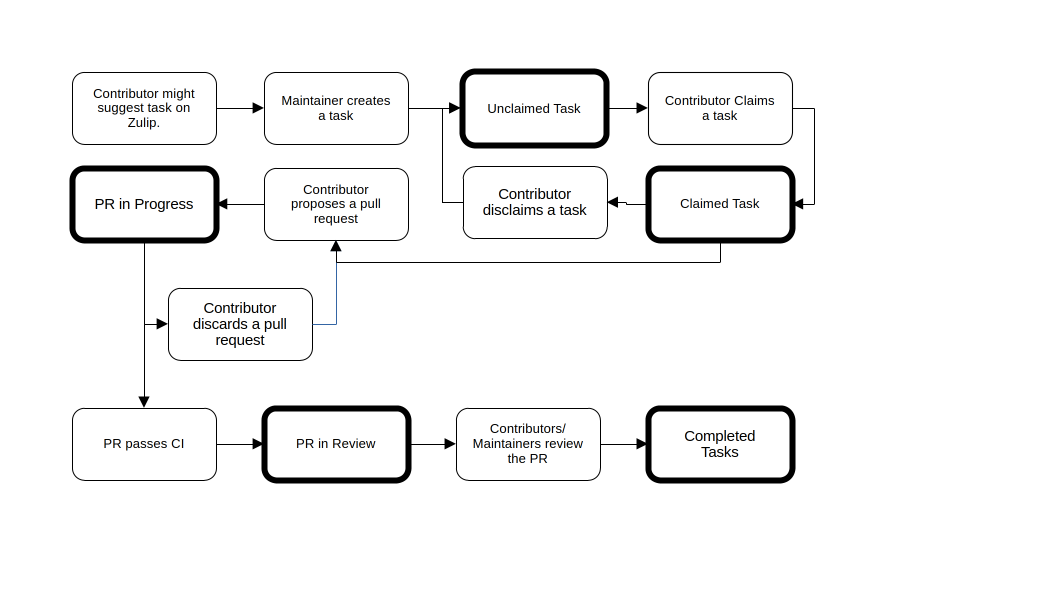
\includegraphics[width=1.0\textwidth]{proj_mgmt_figures/task_flowchart.png}
    \caption{\label{fig:proj_mgmt_flow} A partial flowchart of the automated task management process. Each task corresponds to an issue. A pull request is created to resolve tasks and once a pull request linked to a task is merged, the task is considered complete. The thick boxes represent states of the project dashboard represented by task columns. The movement of tasks between these states is automated by the CI which is triggered upon specific actions performed by contributors on the respective GitHub issues and pull requests. A more detailed description is found in the contributions file of the GitHub file, named\texttt{ CONTRIBUTING.md} by convention.}
\end{figure}

\begin{figure}[t]
    \centering
    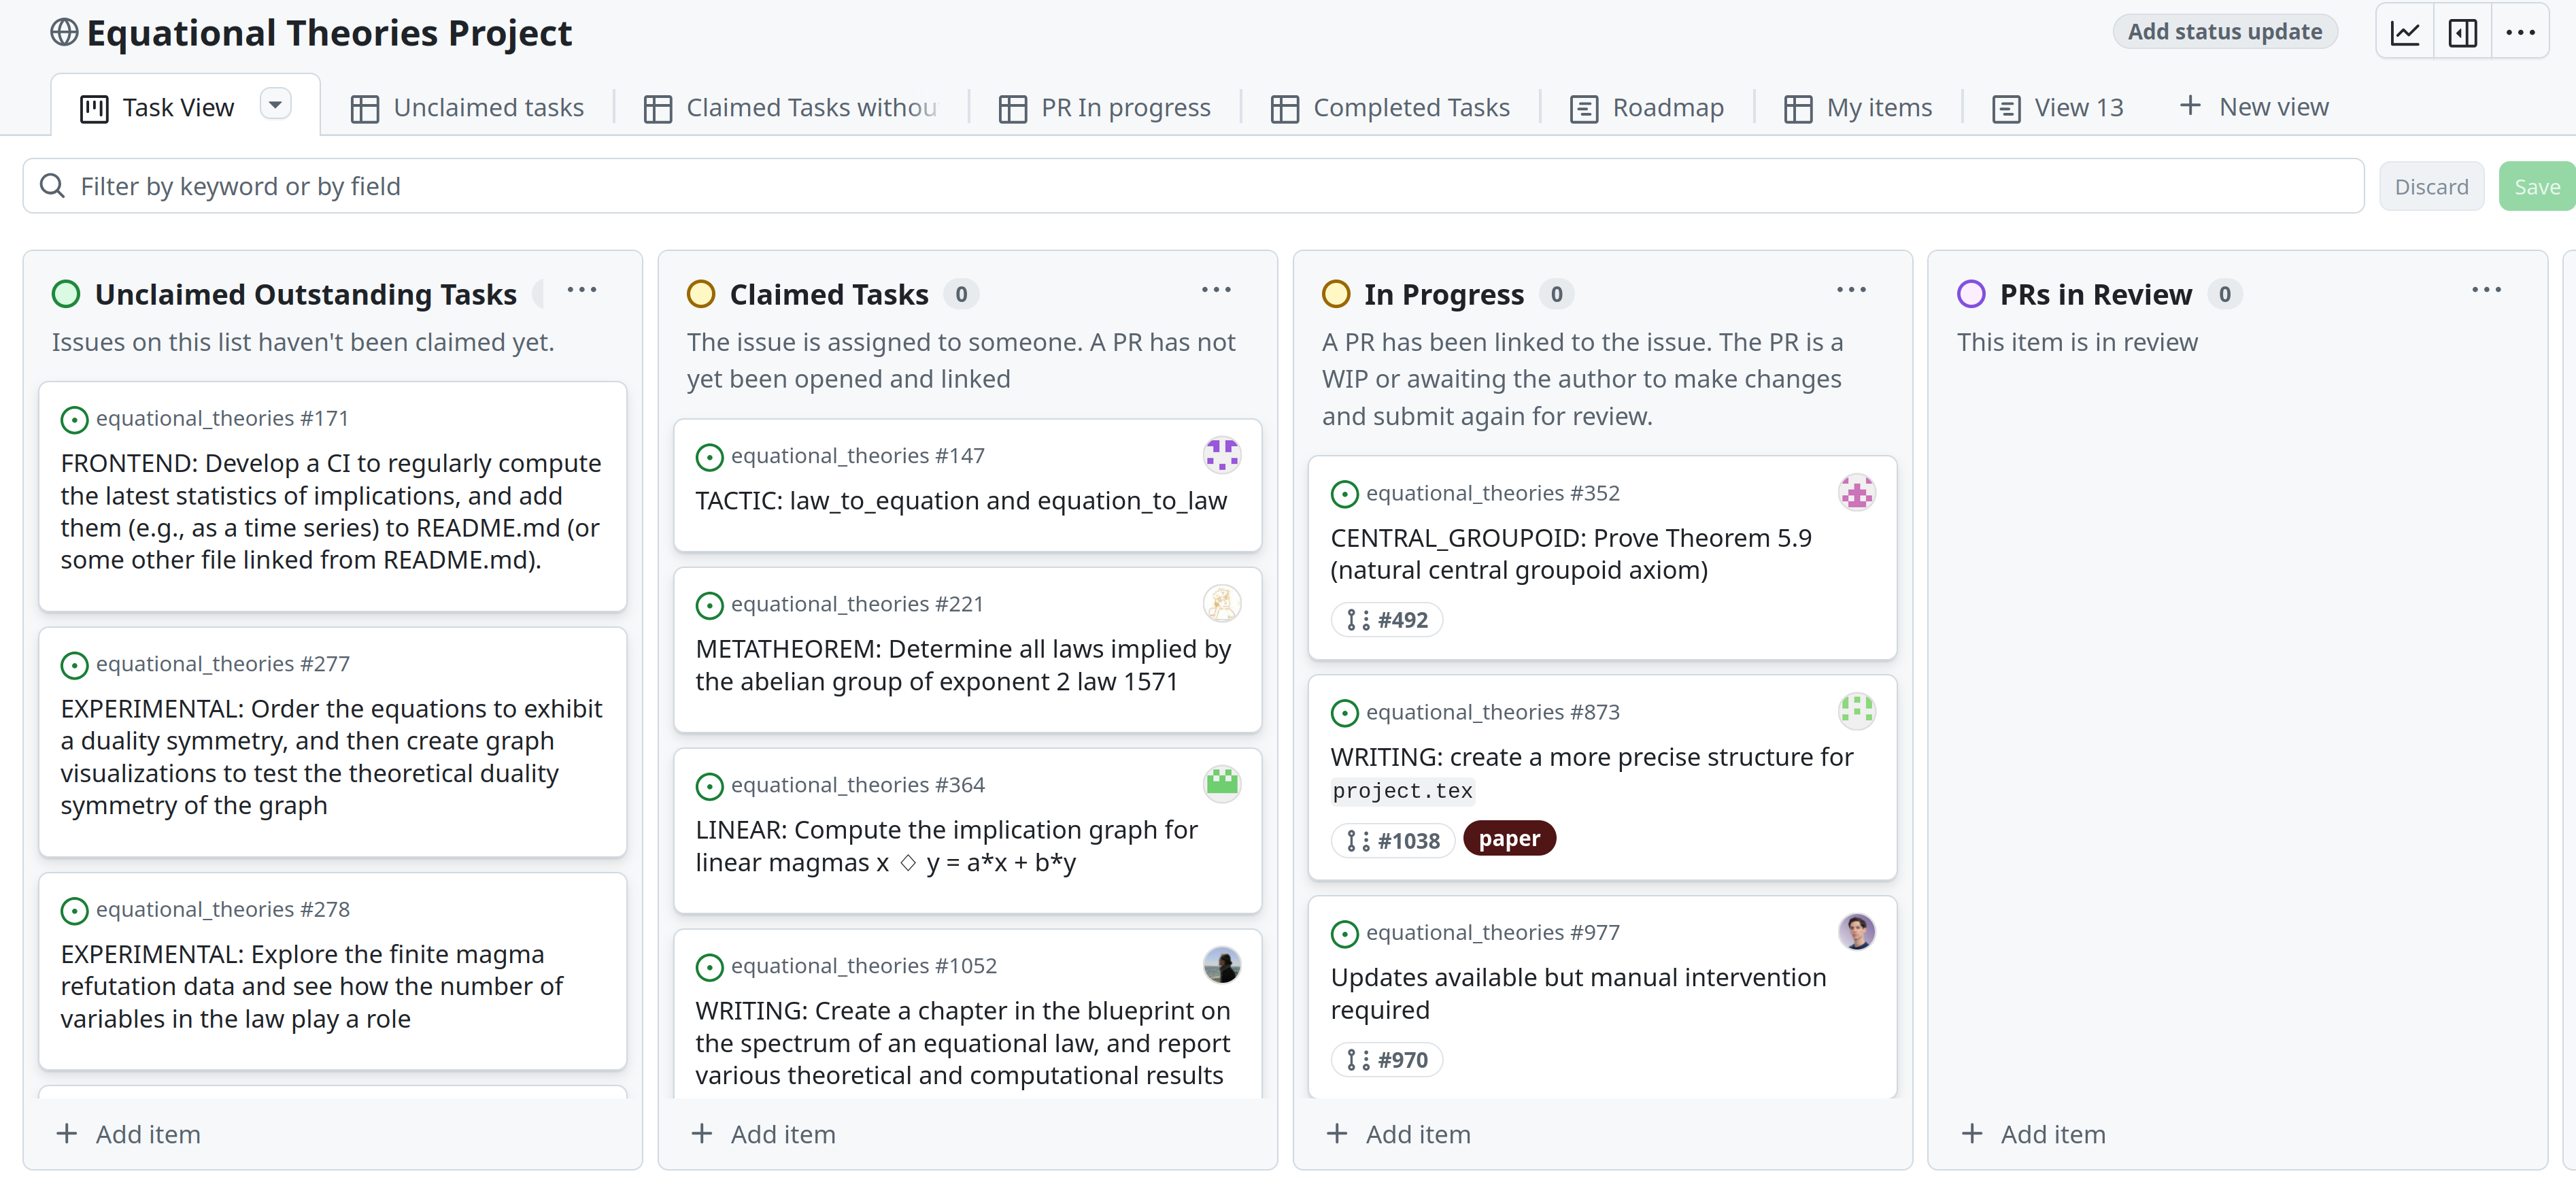
\includegraphics[width=1.0\textwidth]{proj_mgmt_figures/proj_dash_snapshot.png}
    \caption{\label{fig:proj_dashboard} A snapshot of the project dashboard as of July 30th 2025}
\end{figure}
\subsection{Trusting ITPs to Scale Collaboration}
In our project we used the interactive theorem prover (hereon ITP) \emph{Lean} 4 \cite{the_lean4_paper} precisely to address these issues of scaling. The contents of this section are common knowledge in the ITP and ITP-adjacent research communities. The exposition is intended to be useful to a user of ITPs.

At its core, an interactive theorem prover implements an expressive logic, encoded in a suitable choice of mathematical foundations. \emph{Lean} 4 has the calculus of constructions extended by inductive types as its core logic. This logic is sufficiently powerful to express mathematical definitions and theorems for almost all areas of mathematical interest, while being relatively spartan and easy to write proof checkers for. Additionally, modern ITPs provide a convenient programming language which helps express mathematical ideas in a syntax closer to a mathematician's intuition than would be permitted by raw logical terms. A subset of ITPs like \emph{Lean}, \emph{Rocq} (formerly \emph{Coq}), and \emph{Isabelle} go one step further and provide the means to generate proofs through so-called \emph{tactics}. There are usually numerous tactics, each specialised for specific proof generation methods. Among other things, they search mathematical libraries, simplify expressions, and identify lemmas and hypotheses to make progress in proofs. The proofs generated by this overlying programming machinery are terms in the core logical calculus which are checked mechanically by the proof checker. But in a large project, there is more to trust. It helps to understand the nature and limits of trust one can place on ITPs.

For our purposes, \emph{Lean} consists of three pieces:
\begin{enumerate}
    \item A core proof checker called the \emph{kernel}. This checker encodes a typed $\lambda$-calculus that is sufficiently expressive for most mathematical purposes. Without getting into details, theorems are encoded as a formal specification of the intended theorem statement. Proofs are encoded as deduction trees using known lemmata, acceptable axioms, and inference rules. The kernel checks whether this deduction tree constitutes a correct deduction in the context of existing theorems and lemmata, called the \emph{environment}. Once a theorem's proof has been checked, it is added to the environment and can be used for constructing subsequent proofs. In reality, \emph{Lean} allows users some flexibility in adding declarations into its environment without checking their types.
    \item A sophisticated programming language in which users express their definitions and theorems. Programs in this language are said to  be \emph{elaborated} to produce definitions and proofs in the core logic that the kernel can check.
    \item A compiler which compiles executable \emph{Lean} code into reasonably efficient C code.
\end{enumerate}

Of these three pieces, \emph{the kernel is the smallest and most trusted piece}. Programs in the programming language are translated by an \emph{elaborator} to the spartan language of the kernel. In reality the elaborator does much more, but the key takeaways are the following:
\begin{itemize}
    \item The kernel only verifies programs of a very simple barebones language. A proof verified by \emph{Lean} can be trusted \emph{modulo} the correctness of the kernel implementation. This caveat can be usually dropped because, the kernel is also one of the most battle-hardened pieces of an ITP.
    \item The kernel checks proofs against a given specification. This means that if the formal theorem statement itself is flawed or incorrectly uses other definitions, a correct and verified proof of this theorem would be mathematically meaningless. The formal statement of a theorem gives expression to a mathematician's intuition and intention, and as such, the only check against mistakes in this area come from human review. \emph{Lean} cannot offer any guarantees against false statements written by its users or artificial intelligence tools.
    \item The higher level programming language can in-principle, generate arbitrary deductions. Their correctness is ultimately validated by the kernel. This gives the higher level programming language more leeway in generating possibly incorrect deductions.
    \item Ideally the environment only consists of definitions and lemmata already checked by the kernel. Thus their correct usage in the proof of subsequent theorems is valid. However this assumption is often not entirely true in practical implementations of theorem provers for efficiency reasons. In this case, trust in the kernel is restored by replaying each assumption from scratch in the kernel. This can be accomplished by external checkers. Such checkers, which are ideally independent implementations of the \emph{kernel}, can also guard against implementation mistakes in the kernel. In this project we used the environment replay tool \textit{lean4checker} and the \textit{lean4lean} \cite{lean4lean} tool. To our knowledge this was the first such use of the \textit{lean4lean} tool.

\end{itemize}

\begin{remark}
    A bug in the kernel that allows false statements to be proved is usually called a \emph{soundness} bug. Concretely, a soundness bug can be exploited to produce a kernel-certified proof of the proposition $False$. Such bugs are rare but not entirely non-existent. This is distinct from being able to proof $False$ by simply assuming contradictory or false statements. A proof of the proposition $False$ implies a proof of any statement by \emph{ex falso quod libet}.
\end{remark}

Users of \emph{Lean} only interact directly with the higher level programming language and usually get confirmation of the correctness of their proofs through the editor interface. Further, collaborators on a project such as ours are likely to deploy automated tools such as SAT solvers, SMT solvers, first-order theorem provers, and perhaps even modern AI tools. These tools usually produce proof certificates which are imported or inserted into a \emph{Lean} source files. Some modern AI tools are integrated into code editors which might automatically produce or edit even the statements of theorems and the definitions they deal with. Given the limits to trust mentioned above, a productive and useful collaboration using \emph{Lean} also requires a collaboration and verification infrastructure combining human effort and automated tools. It is in this context that we discuss the project infrastructure. It is a concrete answer to the questions posed by one of the authors at the beginning of this project \cite{Tao_blog_Sep_2024} that combines tools from the ITP community and the software engineering community. All these tools already exist. The goal of this exposition is to explain how they address the concerns described above.


\paragraph{\textbf{The non-Lean pieces:}} While \emph{Lean} can check proofs of theorems upto the limitations described above, a project of this scale involves the use of several non-\emph{Lean} tools. For example there are tools which extract the proven implications and anti-implications. There are tools which construct various visualisations. There are also metaprograms which call external automated theorem provers, and extract proof certificates from them to construct a \emph{Lean} proof out of them. In keeping with the garbage-in garbage-out principle, if these tools get spurious inputs and throw spurious outputs, \emph{Lean} can only tell us that the proofs are incorrect after the formal proofs have been translated to \emph{Lean}. It cannot, for instance, stop us from generating a large number of spurious conjectures that misguide contributors because of a simple index error in an array. Further, the continous integration scripts that run \emph{Lean} and check the \emph{Lean} code with external checkers are not formally verified. Such bugs can only be unconvered by empirical testing and user reports. This highlights a basic caveat when using interactive theorem provers. These tools checks something highly specific, a proof, against a specification. Contributors are responsible for the correctness of everything else. This makes the role of organisers and maintainers especially important.

\subsection{The Role of Organisers and Maintainers}
As mentioned before, the correctness of the project depends on a lot of moving pieces, many of which cannot be guaranteed to be correct or functional by \emph{Lean}. In this section, we give a brief description of the variety of tasks that need to be performed by maintainers. We wish to emphasise that the role played by maintainers is akin to that played by the principal investigator and senior postdoctoral researchers in a large experimental project, in that they need to understand the big picture and mathematical details of the project to a reasonable extent and be capable of making highly technical decisions, either themselves, on in consultation with subject experts. Further, they are likely to have limited time to get involved in highly specific details of the project, and while they might make technical contributions, most of their time will be spent managing and organising tasks for other contributors. The role requires a  combination of mathematical research skills and capacity with software engineering tools.

The organisers and maintainers have several tasks in a project such as ours.
\begin{itemize}
    \item They are responsible for monitoring the Zulip chat and onboarding new contributors.
    \item They are responsible for creating new tasks based on requirements and Zulip discussions, and ensuring that they are properly assigned.
    \item They are responsible for ensuring that all the project automation functions smoothly and step in when an issue is detected. It greatly helps to have a geographically distributed set of maintainers across timezones to help fix issues at any time of the day.
    \item They are responsible for reviewing all code, both \emph{Lean} proofs and theorems, and non-\emph{Lean} scripts. This includes ensuring that the automation to build and check proofs, compile the documentation and blueprint, and test and run scripts works smoothly. When necessary they must be willing to step in and build or repair the automation.
    \item They are responsible for reviewing and developing the basic definitions and theorems. As mentioned before, \emph{Lean} takes definitions and theorems for granted. Thus maintainers need to be familiar with both the mathematical content and good ways of expressing this content in  \emph{Lean}. Being proficient in  \emph{Lean} internals is helpful for maintainers in identifying anti-patterns like the use of certain tactics that lead to trusting the  \emph{Lean} compiler, such as \texttt{native\_decide}.
    \item Maintainers are responsible for helping contributors who might get stuck in a proof. Other contributors may also assist in such matters, but ultimately it is up to the maintainers to ensure progress.
    \item Experienced maintainers might also offer suggestions and guidance on how to produce shorter or more elegant proofs.
    \item They are responsible for ensuring that some basic standards are met in proof blocks that make proofs robust to upstream changes. For instance, non-terminal uses of the \texttt{simp} tactic must be replaced with the \texttt{simp only} tactic with an explicit list of lemmas used. Otherwise, changes in the behaviour of upstream libraries can change how the tactic works and affect the correctness of the proof, when the  \emph{Lean} toolchain is updated.
    \item They are responsible for maintaining some record of the progress of the project, Projects on this scale can take a long time and it can become hard to remember how the project progressed. It would be extremely tedious to try to reconstruct real-time impressions long after the fact just from the GitHub commit history and Zulip chat archive. Thus it is extremely helpful if maintainers keep and publish regular logs of activities at a frequency that is proportionate to the scale of activity in the project.In our case, the main organiser maintained a daily log of activities during the busiest part of the project, which became less frequent as the progress rate slowed towards the end.
\end{itemize}

In this project, we were still learning a lot of the aforementioned lessons. A key learning from this project is that it really helps to have a maintainer structure in place before the project begins, rather than inventing one on the fly. Of course, new contributors can be onboarded as maintainers as necessary. But a small maintainer team in the initial stages can hamper proper review processes and result in suboptimal design choices in the  \emph{Lean} formalization that become hard to undo later, as was the case with the aformentioned free magma issue. As another example, the initial list of equations were translated and put into one  \emph{Lean} file as opposed to several. This created excessively large  \emph{Lean} files which could have been managed better with a better file organisation.

In conclusion, we wish to emphasise that as projects scale, the administrative aspects of the project assume non-trivial importance. They require people who are proficient in at least part of the research topic, technical tools, and administrative matters. Setting these processes well in advance of announcing the project and inviting contributors should lead to a smoother project.





\begin{comment}
-- The below should be in the metatheory section.

Use of transitive reduction etc.\ to keep the  \emph{Lean} codebase manageable. Note that the project is large enough that one cannot simply accept arbitrary amounts of  \emph{Lean} code into the codebase, as this could make compilation times explode. Also note somewhere that transitive completion can be viewed as directed graph completion on a doubled graph consisting of laws and their formal negations.
\end{comment}


\section{Counterexample constructions}

In this section we collect the various techniques developed in the ETP to construct counterexamples to various implications $\E \models {\E'}$.

\subsection{Finite magmas}\label{finite-sec}

A finite magma $\Magma$ of size $n$ can be assumed without loss of generality to have carrier $\{1,\dots,n\}$ and described by specifying the multiplication table $\op \colon \{1,\dots,n\} \times \{1,\dots,n\} \to \{1,\dots,n\}$.  By generating a list of all the equational laws $\Eq{j}$, $j=1,\dots,4694$ satisfied by this magma, one can create refutations: if $\Magma \models \Eq{j}$ and $\Magma \not \models \Eq{k}$, then clearly $\Eq{j} \nmodelsfin \Eq{k}$ and hence also $\Eq{j} \nmodels \Eq{k}$.  (As mentioned previously, these statements were organized in Lean using the \texttt{Facts} statement.) It is feasible to brute force over all $\sum_{n=2}^4 n^{n^2} \approx 4.3 \times 10^9$ non-trivial magmas of size at most $4$ to obtain many refutations of this type.
By performing brute force over all magmas up to size $4$, a total of $\num{13632566}$ implications ($61.9\%$ of all implications, and $96.3\%$ of the false ones) can be refuted with $524$ distinct magmas. Of these implications, $\num{13345053}$ were refuted with magmas of size $3$, with the remaining $\num{415293}$ requiring magmas of size $4$. Performing this search took 165 CPU-hours.

However, it is not feasible to exhaustively search over the $5^{5^2} \approx 3 \times 10^{17}$ magmas of size $5$, even after quotienting out by isomorphism and symmetry (which roughly saves a factor of $5! \times 2 = 240$).  Randomly sampling such magmas did not produce significant refutations, as random magmas of size $5$ tended to satisfy few laws, and the set of laws covered were usually also exhibited by smaller magmas.  A more fruitful approach was to randomly sample from magmas with additional properties that encouraged satisfiability of a greater set of laws.  These included linear and quadratic magmas (discussed below), and cancellative magmas.  On the other hand, some classes of magmas, such as commutative magmas, ended up producing a disappointingly small number of additional refutations.

For specific refutations, it was sometimes possible to locate a finite example with an ATP, particularly if one also imposed additional axioms (e.g., an idempotence axiom $x = x \op x$) that one suspected would be useful; see \Cref{automated-sec} for further discussion.  For medium-sized magmas (of size $n=5,6,7,8$), this appeared to be a more efficient approach than brute force exhaustion of all such magmas.

It is a result of Kisielewicz \cite{Kisielewicz} that every law $\Eq{n}$ with $n \leq 4694$ is either equivalent to the singleton law $\Eq{2}$, or else has a non-trivial finite model; in other words, the implications $\Eq{n} \models \Eq{2}$ and $\Eq{n} \modelsfin \Eq{2}$ are equivalent for $n \leq 4694$.  Our brute force search revealed that in the latter case there is always a model of size $2 \leq n \leq 5$, with the lone exception of \eqref{eq1286} (and its dual \eqref{eq2301}), for which the smallest non-trivial finite model was of size $7$, as presented in \Cref{1286-ex} below.  In fact, most of the $\num{4694}$ laws either only had trivial models, or had an size $2$ model, as shown in \Cref{size-table}.
\begin{table}
\centering
\begin{tabular}{ll}
  \hline
Size of smallest non-trivial model & Number of laws \\
\hline
Trivial only & $1496$ \\
$2$ & $3136$ \\
$3$ & $32$ \\
$4$ & $14$ \\
$5$ & $14$ \\
$7$ & $2$\\
\hline
\end{tabular}
\caption{Number of laws of order at most $4$ whose smallest non-trivial model (if any) is of a given size.}\label{size-table}
\end{table}

\begin{remark} The laws satisfied by a given finite magma $\Magma$ need not be finitely axiomatizable.  The smallest example is the three-element magma $\{0,1,2\}$ with $1 \op 2 = 1$, $2 \op 1 = 2 \op 2 = 2$, and $x \op y = 0$ for all other $x,y$ \cite{murskii-1}.  It was also shown in \cite{murskii-2} that ``almost all'' magmas $\Magma$ (in a certain precise sense) are idemprimal\footnote{A magma is idemprimal if every idempotent function is expressed by a term.  This is weaker than being primal (in which \emph{every} function is expressible by a term), but stronger than being quasiprimal (in which the \emph{discriminator} $f(a,b,c)$, defined to equal $c$ if $a=b$ and $a$ otherwise, is expressed by a term); quasiprimality is sufficient to show that all other finite magmas satisfying the laws of $\Magma$ are isomorphic to products of submagmas of $\Magma$.  By combining these observations with \cite{Padmanabhan}, one can also show that quasiprimal finite magmas can be axiomatized by a single equation.  We thank Stanley Burris for these comments, as well as the other references and observations in this remark.}, which implies that their laws are finitely axiomatizable, and all other finite magmas satisfying these laws are isomorphic to powers of $\Magma$.
\end{remark}

\subsection{Linear models}\label{linear-sec}

As it turns out, a particularly fruitful source of counterexamples is the class of \emph{linear magmas}, where the carrier $M$ is a ring (which may be commutative or noncommutative, finite or infinite), and the operation $\op$ is given by $x \op y = ax + by$ for some coefficients $a,b \in M$; one can also generalize this slightly to \emph{affine magmas}, in which the operation is given by $x \op y = ax + by + c$, but for simplicity we shall focus on linear magmas here.  It is easy to see that in a linear magma, any word $w(x_1,\dots,x_n)$ of $n$ indeterminates also takes the linear form
$$ w(x_1,\dots,x_n) = \sum_{i=1}^n P_{w,i}(a,b) x_i$$
for some (possibly noncommutative) polynomial $P_{w,i}$ in $a,b$ with integer coefficients.  Thus, a linear magma will satisfy an equational law $w_1 \formaleq w_2$ if and only if the pair $(a,b)$ lies in the (possibly noncommutative) variety
\begin{equation}\label{variety}
  V_{w_1,w_2}(M) \coloneqq \{ (a,b) \in M \times M: P_{w_1,i}(a,b) = P_{w_2,i}(a,b) \hbox{ for all } i \} \subset M^2.
\end{equation}
As such, a necessary condition for such a law $w_1 \formaleq w_2$ to entail another law $w'_1 \formaleq w'_2$ is that one has the inclusion
$$ V_{w_1,w_2}(M) \subset V_{w'_1,w'_2}(M)
$$
for all rings $M$.  For commutative rings, this criterion can be checked in an automatable fashion by standard Gr\"obner basis techniques; in the noncommutative case one can use methods such as the diamond lemma \cite{diamond-lemma}.

\begin{example}[Commutative counterexample]\label{1286-ex} For the law $x \formaleq y \op (((x \op y) \op x) \op y)$ \eqref{eq1286}, the variety \eqref{variety} can be computed to be
$$ \{ (a,b) \in M \times M: 1 = ba^3+bab, 0 = a + ba^2 b + b^2 \}$$
while the variety for the idempotent law \eqref{eq3} is
$$ \{ (a,b) \in M: a+b=1 \}.$$
Thus, to show that \eqref{eq1286} does not entail \eqref{eq3}, it suffices to locate elements $a,b$ of a ring $M$ for which one has $1 = ba^3+bab$, $0 = a + ba^2 b + b^2$, and $a+b \neq 1$.  Here one can take a commutative example, for instance when $M = \Z/p\Z$ and $(p,a,b) = (11,1,7)$.
\end{example}

\begin{example}[Noncommutative counterexample]\label{1117-ex} For the law $x \formaleq y \op ((y \op (x \op z)) \op z)$ \eqref{eq1117}, the variety \eqref{variety} can be computed to be
$$ \{ (a,b) \in M \times M: 1 = baba, 0 = a+ba^2, 0 = bab^2 + b^2 \}$$
while the variety for $x = (x \op ((x \op x) \op x)) \op x$ \eqref{eq2441} is
$$ \{ (a,b) \in M \times M: 1 = a^2 + aba^2 + abab + ab^2 + b \}.$$
Observe that if $ba = -1$, then $(a,b)$ automatically lies in the first set, and lies in the second set if and only if $(ab+1)(b-1) = 0$.  One can then show that \eqref{eq1117} does not imply \eqref{eq2441} by setting $a = L$, $b = -R$ where $L, R$ are the left and right shift operators respectively on the ring of integer-valued sequences $\Z^\N$.  With some \emph{ad hoc} effort one can convert this example into a less linear, but simpler (and easier to formalize) example, namely the magma with carrier $\Z$ and operation $x \op y = 2x - \lfloor y/2 \rfloor$.
\end{example}

\begin{remark} As essentially observed in \cite{austin}, if there is a commutative linear counterexample to an implication $\E \models {\E'}$, then by the Lefschetz principle this counterexample can be realized in a finite field ${\mathbb F}_q$ for some prime power $q$ (and by the Chebotarev density theorem one can in fact take $q$ to be a prime, so that the carrier is of the form $\Z/p\Z$ for some prime $p$), so that one also has $\E \modelsfin {\E'}$.  As such, we have found that an effective way to refute implications by the commutative linear magma method is to simply perform a brute force search over linear magmas $x \op y = ax + by$ in $\Z/p\Z$ for various triples $(p,a,b)$.

On the other hand, the refutations obtained by noncommutative linear constructions need not have a finite model.  For instance, consider the refutation $\Eq{1117} \nmodels \Eq{2441}$ from \Cref{1117-ex}.  The law \eqref{eq1117} can be rewritten as $L_y R_z L_y R_z x = x$.  This implies that $R_z$ is injective and $L_y$ is surjective for all $y,z$.  For finite magmas $\Magma$, this then implies that the $L_y, R_z$ are in fact invertible, and hence we have also $R_z L_y R_z L_y x = x$, which implies \eqref{eq2441} by setting $x=y=z$.  Thus, the refutation $\Eq{1117} \nmodels \Eq{2441}$ is ``immune'' to finite counterexamples.
\end{remark}

\begin{remark}  One can also consider nonlinear magma models, such as quadratic models $x \op y = ax^2 + bxy + cy^2 + dx + ey + f$ in a cyclic group $\Z/N\Z$.  For small values of $N$, we have found such models somewhat useful in providing additional refutations of implications $\E \modelsfin {\E'}$ beyond what can be achieved by the linear or affine models.  However, as the polynomials associated to a word $w(x_1,\dots,x_n)$ tend to be of high degree (exponential in the order of the word), it becomes quite rare for such models to satisfy a given equation $\E$ when $N$ is large.
\end{remark}

\begin{remark} One can also consider the seemingly more general linear model $x \op y = ax + by$, where the carrier $M$ is now an abelian group, and $a,b$ act on $M$ by homomorphisms, that is to say that they are elements of the endomorphism ring $\mathrm{End}(M)$.  However, this leads to exactly the same varieties \Cref{variety} (where $M$ is now replaced by the endomorphism ring $\mathrm{End}(M)$) and so does not increase the power of the linear model for the purposes of refuting implications.
\end{remark}

On the other hand, there are certainly some refutations $\E \nmodels {\E'}$ of implications that are ``immune'' to both commutative and noncommutative models, in the sense that all such models that satisfy $\E$, also satisfy ${\E'}$.  One such example is the refutation $\Eq{1485} \not \models \Eq{151}$, which we discuss further in \Cref{twisting-sec} below.

\subsection{Translation-invariant models}\label{translation-sec}

It is natural to look for counterexamples amongst magmas that satisfy a large number of symmetries.  One such class of counterexamples are \emph{translation-invariant models}, in which the carrier $M$ is a group, and the left translations of this group form isomorphisms of the magma $\Magma$.  In the case of an abelian group $M = (M,+)$, such models take the form
\begin{equation}\label{xop-add}
  x \op y = x + f(y-x)
\end{equation}
for some function $f \colon M \to M$; in the case of a non-abelian group $M = (M,\cdot)$, such models instead take the form
\begin{equation}\label{xop-mul}
x \op y = x f(x^{-1} y).
\end{equation}
For such models, the verification of an equational law in $n$ variables corresponds to a functional equation for $f$ in $n-1$ variables, as the translation symmetry allows one to normalize one variable to be the identity (say). This can simplify an implication to the point where an explicit counterexample can be found.  These functional equations are trivial to analyze when $n=1$.  For $n=2$, they are not as trivial, but still quite tractable, and has led to several refutations in practice.  The method does not appear to be particularly effective for $n>2$ due to the complexity of the functional equations.

\begin{example}[Abelian example]\label{abex}  For the law $\x \formaleq (\x \op \y) \op ((\x \op \y) \op \y)$ \eqref{eq1648}, we apply the abelian translation-invariant model \Cref{xop-add} with $y=x+h$ to obtain
\begin{align*}
  x \op y &= x + f(h) \\
  (x \op y) \op y &= x + f(h) + f(h-f(h)) \\
  (x \op y) \op ((x \op y) \op y) &= x + f(h) + f(f(h-f(h)))
\end{align*}
so that this model satisfies \eqref{eq1648} if and only if the functional equation
$$f(h) + f(f(h-f(h))) = 0$$
holds for all $h \in M$.  Similarly, the law $\x \formaleq (\x \op (\x \op \y)) \op \y$ \eqref{eq206} is satisfied if and only if
$$ f(f(h)) + f(h - f(f(h))) = 0$$
for all $h \in M$.  One can now check that the function $f \colon \Z \to \Z$ defined by $f(h) \coloneqq - \mathrm{sgn}(h)$ (thus $f(h)$ equals $-1$ when $h$ is positive, $+1$ when $h$ is negative, and $0$ when $h$ is zero) satisfies the first functional equation but not the second, thus establishing that $\Eq{1648} \nmodels \Eq{206}$.
\end{example}

\begin{example}[Non-abelian example]\label{trans-nonab}  We now obtain the opposite refutation $\Eq{206} \nmodels \Eq{1648}$ to \Cref{abex} using the non-abelian translation-invariant model.  By similar calculations to before, we now seek to find a function $f \colon M \to M$ on a non-abelian group $(M,\cdot)$ that satisfies the functional equation
\begin{equation}\label{206-eq}
 f(f(h)) f(f(f(h))^{-1} h) = 1
\end{equation}
for all $h \in M$, but fails to satisfy the functional equation
\begin{equation}\label{1648-eq}
   f(h) f(f(f(h)^{-1} h)) = 1
\end{equation}
for at least one $h \in M$.  Now take $M$ to be the group generated by three generators $a,b,c$ subject to the relations $a^2=b^2=c^2=1$, or equivalently the group of reduced words in $a,b,c$ with no adjacent letters in the word equal.  We define
$$ f(1) = 1, f(a)=b, f(b) = c, f(c) = a$$
and then $f(aw)=a$ for any non-empty reduced word $w$ not starting with $a$, and similarly for $b$ and $c$.  The equation \eqref{206-eq} can be checked directly for $h=1,a,b,c$.  If $h=aw$ with $w$ non-empty, reduced, and not starting with $a$, then $f(f(h))^{-1} = f(f(h)) = b$ and $f(f(f(h))^{-1} h) = f(baw) = b$, giving \eqref{206-eq} in this case, and similarly for cyclic permutations. Meanwhile, \eqref{1648-eq} can be checked to fail for $h=a$.
\end{example}

\begin{remark}  The construction in \Cref{trans-nonab} also has the following more ``geometric'' interpretation.  The carrier $M$ can be viewed as the infinite $3$-regular tree, in which every vertex imposes a cyclic ordering on its $3$ neighbors (for instance, if we embed $M$ as a planar graph, we can use the clockwise ordering).  For $x,y \in M$, we then define $x \op y$ to equal $x$ if $x=y$.  If $y$ is instead a neighbor of $x$, we define $x \op y$ to be the next neighbor of $x$ in the cyclic ordering.  Finally, if $y$ is distance two or more from $x$, we define $x \op y$ to be the neighbor of $x$ that is closest to $y$.  One can then check that this model satisfies \eqref{206-eq} but not \eqref{1648-eq}.
\end{remark}

\begin{remark} These constructions are necessarily infinitary in nature, because \eqref{eq206} and \eqref{eq1648} can be shown to be equivalent for finite magmas. Indeed, \eqref{eq206} can be written as $x = R_y L_x L_x y$, which implies that $R_y$ is surjective, hence injective, on a finite magma; writing $x = R_y z$ we conclude that $R_y z = R_y L_{z \op y} L_{z \op y} y$ and hence $z = L_{z \op y} L_{z \op y} y$, giving \eqref{eq1648}.  The opposite implication is similar (using \eqref{eq1648} to show that $R_y$ is injective, hence surjective), and is left to the reader.
\end{remark}

  Some refutations $\E \nmodels {\E'}$ are ``immune'' by translation-invariant models, in the sense that any translation-invariant model that satisfies $\E$, also satisfies ${\E'}$.  One obstruction is that for such models, the squaring map $S$ is necessarily an invertible map, since $Sx = x + f(0)$ in the abelian case and $Sx = xf(1)$ in the non-abelian case. On the other hand, adding the assumption of invertibility of squares can sometimes force the implication $\E \models {\E'}$ to hold.  For instance, the commutative law $\x \op (\y \op \y) \formaleq (\y \op \y) \op \x$ \eqref{eq4482} for a square and an arbitrary element will imply the full commutative law \eqref{eq43} for translation-invariant models due to the surjectivity of $S$, but does not imply it in general (as one can easily see by considering models where $S$ is constant).

\subsection{The twisting semigroup}\label{twisting-sec}

Suppose one has a magma $\Magma$ satisfying a law $\E$, that also enjoys some endomorphisms $T, U \colon \Magma \to \Magma$.  Then one can ``twist'' the operation $\op$ by $T,U$ to obtain a new magma operation
\begin{equation}\label{twist} x \op' y := Tx \op Uy.
\end{equation}
If one then tests whether this new operation $\op'$ satisfies the same law $\E$ as the original operation $\op$, one will find that this will be the case provided that $T,U$ satisfy a certain set of relations.  The semigroup generated by formal generators $\mathrm{T}, \mathrm{U}$ with these relations will be called the \emph{twisting semigroup} $\operatorname{Twist}_\E$ of $\E$.  This can be best illustrated with some examples.

\begin{example}  We compute the twisting semigroup of $\x \formaleq (\y \op \x) \op (\x \op (\z \op \y))$ \eqref{eq1485}.  We test this law on the operation \eqref{twist}, thus we consider whether
$$x = (y \op' x) \op' (x \op' (z \op' y))$$
holds for all $x,y,z \in M$.  Substituting in \Cref{twist} and using the homomorphism property repeatedly, this reduces to
$$x = (T^2y \op TUx) \op (UTx \op (U^2T z \op U^3y)).$$
If we impose the conditions $TU=UT=\mathrm{id}$, $T^2 = U^3$, then this equation would follow from \eqref{eq1485} (with $x,y,z$ replaced with $TUx=UTx=x$, $T^2 y$, and $U^2 Tz$ respectively).  Thus the twisting semigroup $\operatorname{Twist}_{\Eq{1485}}$ of \eqref{eq1485} is generated by two generators $\mathrm{T}, \mathrm{U}$ subject to the relations $\mathrm{T} \mathrm{U}=\mathrm{U} \mathrm{T} = 1$, $\mathrm{T}^2 = \mathrm{U}^3$.  This is a cyclic group of order $5$, since the relations can be rewritten as $\mathrm{T}^5 = 1$, $\mathrm{U} = \mathrm{T}^{-1}$.

Now consider $\x \formaleq (\x \op \x) \op (\x \op \x)$ \eqref{eq151}.  Applying the same procedure, we arrive at
$$x = (T^2 x \op TUx) \op (UT x \op U^2 x)$$
so the twisting group $\operatorname{Twist}_{\Eq{151}}$ is generated by two generators $\mathrm{T}, \mathrm{U}$ subject to the relations $\mathrm{T} \mathrm{U}=\mathrm{U} \mathrm{T} = \mathrm{T}^2 = \mathrm{U}^2 = 1$.  This is a cyclic group of order $2$, since the relations can be rewritten as $\mathrm{T}^2 = 1$, $\mathrm{U} = \mathrm{T}$.
\end{example}

Suppose the twisting semigroup $\operatorname{Twist}_\E$ is not a quotient of $\operatorname{Twist}_{{\E'}}$, in the sense that the relations that define $\operatorname{Twist}_{{\E'}}$ are not satisfied by the generators of $\operatorname{Twist}_\E$.  Then one can often disprove the implication $\E \models {\E'}$ by attempting the following procedure.
\begin{itemize}
\item First, locate a non-trivial magma $\Magma = (M,\op)$ satisfying the law $\E$.  Then the Cartesian power $M^{\operatorname{Twist}_\E}$ of tuples $(x_W)_{W \in \operatorname{Twist}_\E}$, with the pointwise magma operation, will also satisfy $\E$.
\item Furthermore, this Cartesian power admits two endomorphisms $T, U$ defined by
$$ T (x_W)_{W \in \operatorname{Twist}_\E} = (x_{W \mathrm{T}})_{W \in \operatorname{Twist}_\E};
U (x_W)_{W \in \operatorname{Twist}_\E} = (x_{W \mathrm{U}})_{W \in \operatorname{Twist}_\E},$$
which satisfy the relations defining $\operatorname{Twist}_\E$.
\item We now twist the magma operation $\op$ on $M^{\operatorname{Twist}_\E}$ by $T,U$ to obtain a new magma operation $\op'$ defined by \eqref{twist}, that will still satisfy law $\E$.
\item Because $T, U$ will not satisfy the relations defining $\operatorname{Twist}_{{\E'}}$, it is highly likely that this twisted operation will not satisfy ${\E'}$, thus refuting the implication $\E \models {\E'}$.  If $M$ and the twisting semigroup were finite, this approach should also refute $\E \modelsfin {\E'}$.
\end{itemize}

For instance, a non-trivial finite model for \eqref{eq1485} is given by the finite field $\mathbb{F}_2$ of two elements with the NAND operation $x \op y \coloneqq 1-xy$.  If we twist $\mathbb{F}_2^5$ by the left shift $T(x_i)_{i=1}^5 = (x_{i+1})_{i=1}^5$ and right shift $U(x_i)_{i=1}^5 = (x_{i-1})_{i=1}^5$, where we extend the indices periodically modulo $5$, then the resulting operation
$$ (x_i)_{i=1}^5 \op' (y_i)_{i=1}^5 \coloneqq (1 - x_{i+1} y_{i-1})_{i=1}^5$$
on $\mathbb{F}_2^5$ still satisfies \eqref{eq1485}, but does not satisfy \eqref{eq151}, thus showing that $\Eq{1485} \nmodelsfin \Eq{151}$ and hence $\Eq{1485} \nmodels \Eq{151}$.  This particular implication does not seem to be easily establishable by any of the other methods discussed in this paper.

\subsection{Greedy constructions}\label{greedy-sec}

We have found \emph{greedy extension methods}, or \emph{greedy methods} for short, to be a powerful way to refute implications, especially when the carrier $M$ is allowed to be infinite.  Such constructions have a long history in model theory, with possibly the earliest\footnote{We thank Stanley Burris for this reference.} such construction due to Skolem \cite{skolem}. A basic implementation of this method is as follows.  To build a magma operation $\op \colon M \times M \to M$ that satisfies one law $\E$ but not another ${\E'}$, one can first consider \emph{partial magma operations} $\op \colon \Omega \to M$, defined on some subset $\Omega$ of $M \times M$. Thus $x \op y$ is defined if and only if $(x,y) \in \Omega$. A magma operation is then simply a partial operation which is \emph{total} in the sense that $\Omega = M \times M$.  We say that a partial magma operation is \emph{finitely supported} if $\Omega$ is finite.

In the language of first-order logic (in which functions and relations must be total), it is convenient to view a partial magma operation as a ternary relation $R(x,y,z)$ on $M$ with the axiom that $R(x,y,z) \wedge R(x,y,z') \implies z=z'$ for all $x,y,z \in M$.  The support $\Omega$ is then the set of $(x,y)$ for which $R(x,y,z)$ holds for some (necessarily unique) $z$, which one can then take to be the definition of $z = x \op y$.

We say that one partial operation $\op' \colon \Omega' \to M$ \emph{extends} another $\op \colon \Omega \to M$ if $\Omega'$ contains $\Omega$, and $x \op y = x \op' y$ whenever $x \op y$ (and hence $x \op' y$) are defined. Given a sequence $\op_n \colon \Omega_n \to M$ of partial operations, each of which is an extension of the previous, we can define the \emph{direct limit} $\op_\infty \colon \bigcup_n \Omega_n \to M$ to be the partial operation defined by $x \op_\infty y \coloneqq x \op_n y$ whenever $(x,y) \in \Omega_n$.

Abstractly, the greedy algorithm strategy can now be described as follows.

\begin{theorem}[Abstract greedy algorithm]\label{greedy-abstract} Let $\E,{\E'}$ be equational laws, and let $\Gamma$ be a theory of first-order sentences regarding a  partial magma operations $\op \colon \Omega \to M$ on a carrier $M$.  Assume the following axioms:
\begin{itemize}
  \item[(i)] (Seed) There exists a finitely supported partial magma operation $\op_0 \colon \Omega_0 \to M$ satisfying $\Gamma$ that contradicts ${\E'}$, in the sense that there is some assignment of variables in ${\E'}$ in $M$ such that both sides of ${\E'}$ are defined using $\op_0$, but not equal to each other.
  \item[(ii)]  (Soundness)  If $\op_n \colon \Omega_n \to M$ is a sequence of partial magma operations satisfying $\Gamma$ with each $\op_{n+1}$ an extension of $\op_n$, and the direct limit $\op_\infty$ is total, then this limit satisfies $\E$.
  \item[(iii)] (Greedy extension)  If $\op \colon \Omega \to M$ is a finitely supported partial magma operation satisfying $\Gamma$, and $a,b \in M$, then there exists a finitely supported extension $\op' \colon \Omega' \to M'$ of $\op$ to a possibly larger carrier $M'$, and also satisfying $\Gamma$, such that $a \op' b$ is defined.
\end{itemize}
Then $\E \nmodels {\E'}$.
\end{theorem}

We remark that this greedy method seems to be inherently infinitary in nature, and does not seem well adapted to refute finite magma implications $\E \modelsfin {\E'}$.

\begin{proof}  We work on the countably infinite carrier $\N$.  By embedding the finitely supported operation $\op_0$ from axiom (i) into $\N$, we can assume without loss of generality that $\op_0$ has carrier $\N$.  By similar relabeling, we can assume in (iii) that $M' = M$ when $M=\N$, since any elements of $M' \backslash \N$ that
appear in $\Omega'$ can simply be reassigned to natural numbers that did not previously appear in $\Omega$.  We well-order the pairs in $\N \times \N$ by $(a_n,b_n)$ for $n=1,2,\dots$.  Iterating (iii) starting from $\op_0$, we can thus create a sequence of finitely supported magma operations $\op_0, \op_1, \dots$ on $\N$ satisfying $\Gamma$, with each $\op_{n+1}$ an extension of $\op_n$, and $a_n \op_n b_n$ defined for all $n \geq 1$.  Then the direct limit $\op_\infty$ of these operations is total, and does not satisfy ${\E'}$ thanks to axiom (i).  On the other hand, by axiom (ii) it satisfies $\E$, and the claim follows.
\end{proof}

We refer to $\Gamma$ as the \emph{rule set} for the greedy extension method. To apply \Cref{greedy-abstract} to obtain a refutation $\E \models {\E'}$, we have found the following trial-and-error method to work well in practice:
\begin{itemize}
\item[1.] Start with a minimal rule set $\Gamma$ that has just enough axioms to imply the soundness property for the given hypothesis $\E$.
\item[2.] Attempt to establish the greedy extension property for this rule set by setting $a \op' b$ equal to a new element $c \not \in M$, and then defining additional values of $\op'$ as necessary to recover the axioms of $\Gamma'$.
\item[3.]  If this can be done in all cases, then locate a seed $\op_0$ refuting the given target ${\E'}$, and \texttt{STOP}.
\item[4.]  If there is an obstruction (often due to a ``collision'' in which a given operation $x \op' y$ is required to equal two different values), add one or more rules to $\Gamma$ to avoid this obstruction, and return to Step 2.
\end{itemize}

As an example, we present

\begin{proposition}[$\Eq{73}$ does not imply $\Eq{4380}$]\label{73-4380} The law $\x \formaleq \y \op (\y \op (\x \op \y))$ \eqref{eq73} does not imply $\x \op (\x \op \x) \formaleq (\x \op \x) \op \x$ \eqref{eq4380}.
\end{proposition}

\begin{proof} To build a rule set $\Gamma$ that will imply \eqref{eq73} when total, a natural first choice would be the single rule
\begin{itemize}
\item[1.] If $y \op (x \op y)$ is defined, then $y \op (y \op (x \op y))$ is defined and equal to $x$.
\end{itemize}
However, the greedy algorithm will fail just with this rule: if the partial operation has $x \op y$ and $z \op y$ both equal to some $w$ for some $x \neq z$, then any attempt to assign a value to $y \op (y \op w)$ will lead to a contradiction, as the above rule will force $y \op w$ to equal both $x$ and $z$.  Indeed, it is clear that \eqref{eq73} forces all the right translation operators $R_y$ to be injective.  We therefore add this as an additional rule:
\begin{itemize}
\item[2.] If $x \op y$ and $z \op y$ are defined and equal, then $x=z$.
\end{itemize}
To avoid some unwanted edge cases, it is also convenient to impose the additional rule
\begin{itemize}
  \item[3.] If $x \op y$ is defined, it is not equal to $y$.
\end{itemize}
Unlike Rule 2, this rule is not forced by \eqref{eq73}, but can be enforced as part of the greedy construction.

The ruleset clearly satisfies the soundness axiom (ii) of \Cref{greedy-abstract}.  We now verify the greedy extension axiom (iii).  Let $\Omega,a,b$ be as in that axiom. We may assume that $a \op b$ is undefined, since we are done otherwise. We adjoin a new element $c$ to $M$ to create $M'$, and set $a \op' b = c$.  If we also have $b = d \op a$ for some $d$ (unique by Rule 2, and only possible for $a \neq b$ by Rule 3), set $a \op' c = d$ (this is necessary to retain Rule 1).  Of course, we also set $x \op' y = x \op y$ whenever $x \op y$ is already defined.

Since $c \not \in M$, it is clear that $\op'$ is a finitely supported partial magma operation on $M'$.  It is also clear that $\op'$ satisfies Rule 2 and Rule 3.   Now we case check Rule 1:
\begin{itemize}
\item Case 1: $x=c$ or $y=c$.  Not possible since no left multiplication with $c$ is defined.
\item Case 2: $x \op' y = c$.  Only possible when $x = a$, $y = b$, but then $y \op' (x \op' y)$ is undefined since $y = b \neq a$ if $d$ is defined.
\item Case 3. $y \op' (x \op' y) = c$.  Only possible when $y=a$ and $x=d$, and holds in this case.
\item Case 4: $x, y, x \op' y, y \op' (x \op' y) \neq c$: In this case $\op'=\op$ on all pairs, so the claim reduces to Rule 1 for $\op$, which holds by the induction hypothesis.
\end{itemize}
To conclude, we need to locate a seed $\op_0$ satisfying Rules 1,2,3 and containing a counterexample to \eqref{eq4380}.  One simple example is the carrier $\{0,1,2,3\}$ with $0 \op_0 0 = 1$, $0 \op_0 1 = 2$, $0 \op_0 2 = 0$, $1 \op_0 0 = 3$.
\end{proof}

This method is not guaranteed to halt in finite time, as there may be increasingly lengthy sets of rules one has to add to $\Gamma$ to avoid collisions.  However, in practice we have found many of the refutations that could not be resolved by simpler techniques to be amenable to this method (or variants thereof, as discussed below).

One can automate the above procedure by using ATPs (or SAT solvers) to locate new rules that are necessary and sufficient to resolve any potential collision (and which, \emph{a posteriori}, can be seen to be necessarily consequences of the law $\E$).  The seed-finding step (Step 3) is particularly easy to automate, and can also often be done by hand.  In some cases, the SAT solver calculations provided by these methods were difficult to formalize efficiently in Lean, and so we elected in some cases to replace computer-generated rulesets with shorter human-generated versions in preparation for the formalization step.

However, in some cases we have found it necessary to add ``inspired'' choices of rules that were not forced by the initial hypothesis $\E$, but which simplified the analysis by removing problematic classes of collisions from consideration.  We were unable to fully automate the process of guessing such choices; however, we found ATPs very useful for testing any proposed such guess.  In particular, if an ATP was able to show that the existing ruleset, together with a proposed new rule $A$, implied ${\E'}$, then this clearly indicated that one should not add $A$ to the rule set $\Gamma$.  Conversely, if an ATP failed to establish such an implication, this was evidence that this was a ``safe'' rule to impose.

We also found that human verification of the greedy extension property was a highly error-prone process, as the case analysis often included many delicate edge cases that were easy to overlook.  Both ATPs and the Lean formalization therefore played a crucial role in verifying the human-written greedy arguments, often revealing important gaps in those arguments that required either minor or major revisions to the rule set.

The greedy method can also be combined with the translation-invariant method, both in abelian and non-abelian settings. For instance, we can modify the proof of \Cref{greedy-abstract} to obtain the following variant:

\begin{theorem}[Noncommutative translation-invariant greedy algorithm]\label{nc-greedy-abstract} Let $F,F'$ be functional equations on groups, and let $\Gamma$ be a theory of first-order sentences regarding a partial function $f \colon \Omega \to G$ on a group $G = (G,\cdot)$.  Assume the following axioms:
  \begin{itemize}
    \item[(i)] (Seed) There exists a finitely supported partial function $f_0 \colon \Omega_0 \to G$ satisfying $\Gamma$ that contradicts $F'$, in the sense that there is some assignment of variables in $F'$ in $G$ such that both sides of $F'$ are defined using $f_0$, but not equal to each other.
    \item[(ii)]  (Soundness)  If $f_n \colon \Omega_n \to G$ is a sequence of partial functions satisfying $\Gamma$ with each $f_{n+1}$ an extension of $f_n$, and the direct limit $f_\infty$ is total, then this limit satisfies $F$.
    \item[(iii)] (Greedy extension)  If $f \colon \Omega \to G$ is a finitely supported partial function satisfying $\Gamma$, and $a \in G$, then there exists a finitely supported extension $f' \colon \Omega' \to G'$ of $f$ to a possibly larger group $G'$, and also satisfying $\Gamma$, such that $f'(a)$ is defined.
  \end{itemize}
  Then $F \nmodels F'$.
\end{theorem}

One can of course also develop an abelian analogue of the above theorem, in which $G = (G,+)$ and $G' = (G',+)$ are now required to be abelian.  We can then give an alternate proof of \Cref{73-4380} as follows:

\begin{proof}[Second proof of \Cref{73-4380}] (Sketch)  The functional equations associated to \eqref{eq73} and \eqref{eq4380} are
$f^2(h^{-1} f(h)) =h^{-1}$ and $f^2(1) = f(1) f(f(1)^{-1})$ respectively.  We apply \Cref{nc-greedy-abstract} with the following ruleset:
\begin{itemize}
  \item[1.]  If $f(h^{-1} f(h))$ is defined, then $f^2(h^{-1} f(h))$ is defined and equal to $h^{-1}$.
  \item[2.]  If $h^{-1} f(h)$ and $k^{-1} f(k)$ are defined and equal, then $h=k$.
  \item[3.]  If $f(h)$ is defined, it is not equal to $h$.
\end{itemize}
Axiom (ii) is clear.  To verify axiom (iii), we can assume $f(h)$ is undefined, then adjoin an element $c$ freely to $G$ to create a larger group $G'$, and set $f'(h) = c$.  If $h = k^{-1} f(k)$ for some $k$ (which is unique by Rule 2, and only possible for $h \neq 1$ by Rule 3), then also set $f'(c) = k^{-1}$.  One can then check that axiom (iii) is satisfied.  For axiom (i), take $G$ to be a free cyclic group with one generator $a$, and set $f(1) = a$, $f(a) = a^3$, $f(a^3) = 1$, $f(a^{-1}) = a^3$ (say).
\end{proof}

More complex (and \emph{ad hoc}) variants of the greedy algorithm are possible.  In some cases, we were not able to preserve the finitely supported nature of the partial operation or partial function, and needed to extend that partial object at an infinite number of values at each step.  In other cases, one also had to add additional temporary data during the greedy process to record tasks that one wished to attend to at a later stage of the process, but could not handle immediately because it was awaiting some other operation to become well-defined.  We will not attempt to survey all possible variants of this method here, but refer the reader to the ETP blueprint for further examples.

\subsection{Modifying base models}\label{modify-base}

A general technique that we have found useful in obtaining a refutation such as $\E \nmodels {\E'}$ is to start with a simple base model $\Magma = (M,\op)$ that satisfies both $\E$ and ${\E'}$, and modify it in various ways to preserve $\E$, but create a violation of ${\E'}$.  There are many such possible modifications, but three general ways that have proven effective are as follows:

\begin{itemize}
  \item[(i)]  Modify the magma operation $\op \colon M \times M \to M$ on a small set in order to violate ${\E'}$, and then make further modifications as needed to recover $\E$.
  \item[(ii)]  Construct an \emph{extension} $\MagmaN$ of $\Magma$, equipped with a surjective magma homomorphism $\pi: \MagmaN \to \Magma$, and defined in terms of some additional data.  Then solve for that data in such a way that $N$ satisfies $\E$ but not ${\E'}$.
  \item[(iii)]  Construct an \emph{enlargement} $\Magma' = (M',\op')$ of $\Magma = (M,\op)$, which is a magma that contains $\Magma$ as a submagma.  One needs to construct the multiplication table $\op$ on $(M' \times M') \backslash (M \times M)$ in order to retain $\E$ but disprove ${\E'}$.
\end{itemize}

One appealing case of (ii) that our project discovered, involving a ``magma cohomology'' analogous to (abelian) group cohomology, is that of an \emph{affine} extension of a magma ${\mathcal G} = (G,\op_G)$ by another magma $(M,\op_M)$ which is an abelian group $M$ with a linear magma operation $s \op_M t \coloneqq as + bt$ for some endomorphisms $a,b \in \mathrm{End}(M)$.  One can then consider extensions with carrier $G \times M$ and magma operation
\begin{equation}\label{xsyt}
 (x, s) \op (y, t) \coloneqq (x \op_G y, s \op_M t + f(x,y))
\end{equation}
for some function $f \colon G \times G \to M$.  If $(M,\op_M)$ and $(G,\op_G)$ already satisfy a law $\E$, then this extension will also satisfy $\E$ if and only if $f$ satisfies a certain ``cocycle equation'', which is a linear equation on $f$.  One can then sometimes use linear algebra to locate an $f$ that satisfies the cocycle equation for one law $\E$ but not another ${\E'}$, thus refuting the implication $\E \models {\E'}$.  An example is as follows:

\begin{proposition}[$\Eq{1110}$ does not imply $\Eq{1629}$]\label{1110-1629} The law $\x \formaleq \y \op ((\y \op (\x \op \x)) \op \y)$ \eqref{eq1110} does not imply $\x \formaleq (\x \op \x) \op ((\x \op \x) \op \x)$ \eqref{eq1629}, even for finite magmas.
\end{proposition}

\begin{proof}  (Sketch) Using the linear ansatz, we find that \eqref{eq1110} has a model $\Magma$ with carrier $\F_5$ (the finite field $\Z/5\Z$) with operation $x \op y = 3x-y$.  We then apply the ansatz \eqref{xsyt} with $G=M$.  One then finds that this operation  \eqref{eq1110} if $f \colon \F_5 \times \F_5 \to \F_5$  the cocycle equation
  $$3f(x,x) - 3f(y,2x) - f(3y-2x,y) + f(y,3y-x) = 0$$
for all $x,y \in \F_5$, and satisfies \eqref{eq1629} if $f$ satisfies the cocycle equation
$$ f(2x,0) - f(2x,2x) = 0$$
for all $x \in \F_5$.  A routine symbolic algebra package computation reveals that the space of $f$ that satisfies the former equation is a six-dimensional vector space over $\F_5$, which is not contained in the solution space of the latter equation, giving the claim.
In fact, since these equations preserve the space of homogeneous polynomials of a fixed degree, one can use linear algebra to locate an example that is a homogeneous polynomial; one explicit choice is
\[
f(x,y) = y^5 +xy^4 + x^2y^3 +3x^3 y^2 + 3x^4 y. \qedhere
\]
\end{proof}

It may be of interest to develop this theory of ``magma cohomology'' further, for instance by defining higher order magma cohomology groups.

Now we give an example of how method (ii) can be combined with method (i).

\begin{proposition}[$\Eq{1659}$ does not imply $\Eq{4315}$]\label{1659-4315} The law $\x \formaleq (\x \op \y) \op ((\y \op \y) \op \z)$ \eqref{eq1659} does not imply $\x \op (\y \op \x) \formaleq \x \op (\y \op \z)$ \eqref{eq4315}.
\end{proposition}

\begin{proof}  There are two simple models for \eqref{eq1659}: the model $G$ with carrier $\Z/2\Z$ and operation $x \op y = x+1$, and the model $\Magma$ with carrier $\Z$ and operation $x \op y = x$.  Using the ansatz \eqref{xsyt}, one can soon discover that one obtains a magma operation $\op: (G \times \Z) \times (G \times \Z) \to G \times \Z$ with $f(0,0)=f(1,0)=0$, $f(0,1)=-1$, and $f(1,1)=1$.  This model still  \eqref{eq4315}. However, we can create a modification $\op'$ of $\op$ as follows.  We will seek to violate \eqref{eq4315} at $x = (0,0)$, $y = (0,0)$, $z = (1,0)$, thus we want
$$ (0,0) \op' ((0,0) \op' (0,0)) \neq (0,0) \op' ((0,0) \op' (1,0)).$$
We have $(0,0) \op (0,0) = (1,0)$ and $(0,0) \op (1,0) = (1,-1)$.  One can try to force the counterexample by setting $(0,0) \op' (1,0)$ to equal $(0,0)$ instead of $(1,-1)$. However, if this is the only change we make, then we no longer satisfy \eqref{eq1659}, since
$$ (1,0) \neq ((0,0) \op' (1,0)) \op' (((1,0) \op' (1,0)) \op' (1,t))$$
for any $t \in \N \backslash \{0\}$. But these are the only counterexamples created involving elements in the subset $G \times \N$ of $G \times \Z$; and if one then sets $(0,0) \op' (1,t) = (0,0)$ for \emph{all} $t \in \N$, and then restricts to $G \times \N$ (which is now closed under $\op'$), then one can check that the modified operation $\op'$ on this submagma now  \eqref{eq1659} but not \eqref{eq4315} as required.
Incidentally, this submagma is isomorphic to the magma $\Magma'=(\Z,\op'')$ with $m\op''n=-m$ for $n<0$ and $m\op''n=-m-1$ for $n\geq 0$ under the bijection that maps $(0,s)$ to $s$ and $(1,s)$ to $-s-1$.
\end{proof}

The specific law $\x \formaleq \x \op ((\y \op \z) \op (\x \op \z))$ \eqref{eq854} turned out to be somewhat ``mutable'', in the sense that one can often change a small number
 of entries in the multiplication table of a finite magma satisfying this law, or add rows and columns to the table,
 in ways that preserve the law \eqref{eq854}.  This makes the law amenable to methods (i) and (iii) to construct new models of this equation that
 refute various implications  $\eqref{eq854} \nmodelsfin \E$, for instance by starting with a model that already refuted some stronger law ${\E'}$, and then attempting to modify it
 (possibly with ATP assistance) by some combination of methods (i) and (iii) to produce a model that violates $\E$.

 Some heuristics loosely inspired by discrete-time dynamical systems proved helpful.
 The idea is to generate a sequence of magmas, each of which is generated from the previous entry by applying various operations expected to increase the likelihood of
 finding a refutation.  This is similar to the greedy methods in \ref{greedy-sec}, except that we require our resulting magma to be finite and completely
 defined, and our transformations need not be deterministic.  Note that, since the goal is simply to find a finite model, and given such a candidate we can easily
 determine whether it works, we are not limited to operations we can rigorously justify.  SAT solvers like
 \emph{Glucose}~\cite{DBLP:conf/ijcai/AudemardS09,DBLP:conf/cp/AudemardS12} inspired by the earlier \emph{MiniSAT}~\cite{DBLP:conf/sat/EenS03},
 via convenient interfaces like \emph{PySAT}~\cite{imms-sat18, itk-sat24}, counterexample finders like \emph{Mace4}~\cite{prover9-mace4}, and more general ATPs like
 \emph{Vampire}~\cite{DBLP:conf/cav/KovacsV13} which can be used as solvers, all succeeded in finding useful magmas following this approach.

 For example, one operation we can apply is fixing a random subset of the elements of the magma table while leaving the remainder unspecified,
 and asking an ATP to find a magma which satisfies \eqref{eq854} while preserving the fixed values.
 If in fact $\Eq{854} \nmodelsfin \E$, then the ATP may complete the table to a solution that violates $\E$ as desired.  In some cases,
 it appears that the magma entries can be sufficiently coupled that unless a large fraction of the values is removed,
 every $\Eq{854}$-satisfying solution also satisfies $\E$.
 We can insert a known violation of $\E$ into the magma cells we have emptied, hoping that a consistent completion still exists.
 Another approach, by analogy with slowly introducing forcing terms into numerical integrations while preserving adiabatic invariants, is to impose selected
 implications of a given equation without directly enforcing the equation itself.  This can gradually drive the magmas in the
 sequence toward fewer violations of a given equation without immediately imposing it.

Combining several of these techniques allowed us to find refutations for
$$\Eq{854} \nmodelsfin \Eq{413}, \Eq{1045}, \Eq{1055}, \Eq{3316}, \Eq{3925}.$$
 We started with a magma which satisfied $\Eq{854}$ and $\Eq{413}$ but had an $\Eq{10}$ violation.
After using it as a seed to generate larger magmas with more $\Eq{10}$ violations (using \emph{Vampire}),
randomly removing portions of those magmas and attempting to complete them to models that violated $\E$ eventually succeeded.

Note that these approaches have their limitations.  To be effective, it must be easy to move between different
states, which usually involves finding a magma satisfying the equation of interest or at least some related one.
Equations for which finite magmas are difficult to find (e.g.\ \eqref{eq677}), whether because of absolute rarity or the numerical challenges
that our ATPs have in finding them without taking advantage of a structural ansatz, appear resistant to these methods in practice.

Another way to utilize (iii), which proved useful for laws that involved the squaring operator $S$, was to adopt a ``squares first'' approach in which one selected a base model $S\Magma = (SM,\op)$ to serve as the set of squares, then extend it to a larger model $\Magma$ with carrier $M = SM \uplus N$ by first determining what the multiplication map should be on the diagonal $\{ (x,x): x\in N\}$ (i.e., to determine the squaring map $S \colon N \to SM$), together with the values on the blocks $SM \times N$, $N \times SM$, and then finally resolve the remaining values on the $N \times N$ block.  Often, versions of the greedy algorithm are useful for each of these stages of the construction.  The precise details are quite technical, particularly for the law $\x \formaleq (\y \op \y) \op ((\y \op \x) \op \y)$ \eqref{eq1729}, which was the last of the equations whose implications were settled by the ETP.  We refer the reader to the ETP blueprint for further details.


\section{Syntactic arguments}\label{syntactic-sec}

Many proofs or refutations of implications (or equivalences) between two equational laws $E,E'$ can be obtained from the syntactic form of the equation.  We discuss some techniques here that were useful in the ETP.

\subsection{Simple rewrites}\label{rewrite-sec}

Many equational laws $E'$ can be formally deduced from a given law $E$ by applying the \emph{Lean} \texttt{rw} tactic to rewrite $E'$ repeatedly by some forward or backward application of $E$ applied to arguments that match some portion of $E$.  For instance, the commutative law \eqref{eq43} clearly implies $\x \op (\y \op \z) \formaleq (\y \op \z) \op \x$ \eqref{eq4531}
by a single such rewrite.  A brute force application of such rewrite methods is already able to directly generate about $\num{15000}$ such implications, including many equivalences to the singleton law \eqref{eq2} and the constant law \eqref{eq46}.  After applying transitive closure, this generates about four million further such implications.

A simple observation that already generates a reasonable number of equivalences is that any equation of the form $\x \formaleq f(\y,\z,\dots)$ necessarily is equivalent to the trivial law $\x \formaleq \y$, by transitivity; similarly, an equation of the form $f(\x,\y) \formaleq g(\z,\w,\dots)$ implies $f(\x,\y) \formaleq f(\x',\y')$; and so forth.  Equivalences of this form were useful early in the project by cutting down the number of distinct equivalence classes of laws that needed to be studied.

\subsection{Matching invariants}

Fix an alphabet $X$. A \emph{matching invariant} is an assignment $I \colon \Magma_X \to {\mathcal I}$ of an object $I(w) \in {\mathcal I}$ in some space ${\mathcal I}$ to each word $w \in \Magma_X$ with the property that if an equational law $w_1 \formaleq w_2$ has matching invariants $I(w_1)=I(w_2)$, then the same matching $I(w'_1) = I(w'_2)$ holds for any consequence $w'_1 \formaleq w'_2$.  In particular, if one law $I(w_1)=I(w_2)$ and $I(w'_1) \neq I(w'_2)$, then the law $w_1 \formaleq w_2$ does not imply the law $w'_1 \formaleq w'_2$.

A simple example of a matching invariant is the multiplicity $(n_x)_{x \in X}$ of variables of a word: if $w_1,w_2$ have all variables $x$ appear the same number of times $n_x$ in both words, then any rewriting of a word $w$ using the law $w_1 \formaleq w_2$ will preserve this property.  Hence, if $w'_1, w'_2$ do not have that each variable appear the same number of times in both words, then $w_1 \formaleq w_2$ cannot imply $w'_1 \formaleq w'_2$.  For instance, the commutative law \eqref{eq43} cannot imply the left-absorptive law \eqref{eq4}.

One source of matching invariants comes from the free magma $\Magma_{X,\Gamma}$ of a theory:

\begin{proposition}[Free magmas and matching invariants]\label{free-inv}  Let $\iota_{X,\Gamma} \colon X \to \Magma_{X,\Gamma}$ be the map associated to the free magma $\Magma_{X,\Gamma}$ for a theory $\Gamma$.  Then the map $I \colon \Magma_X \to \Magma_{X,\Gamma}$ defined by $I(w) \coloneqq \varphi_{\iota_{X,\Gamma}}(w)$ is an invariant.
\end{proposition}

\begin{proof}  Suppose that $w_1 \formaleq w_2$ entails $w'_1 \formaleq w'_2$, and that $I(w_1) = I(w_2)$.  For any $f \colon X \to \Magma_{X,\Gamma}$, the two maps $\varphi_f, \varphi_{f,\Gamma} \circ \varphi_{\iota_{X,\Gamma}} \colon \Magma_X \to \Magma_{X,\Gamma}$ are both homomorphisms that extend $f$, hence agree by the universal property of $\Magma_X$, as displayed by the following commutative diagram:
\[\begin{tikzcd}
	&& X \\
	\\
	{\Magma_X} && {\Magma_{X,\Gamma}} && {\Magma_{X,\Gamma}}
	\arrow[hook, from=1-3, to=3-1]
	\arrow["{\iota_{X,\Gamma}}", pos=0.7, left, from=1-3, to=3-3]
	\arrow["f", pos=0.7, above, from=1-3, to=3-5]
	\arrow["{I = \varphi_{\iota_{X,\Gamma}}}", pos=0.6, above, from=3-1, to=3-3]
	\arrow["{\varphi_f}"', curve={height=18pt}, pos=0.6, below, from=3-1, to=3-5]
	\arrow["{\varphi_{f,\Gamma}}", pos=0.5, above, from=3-3, to=3-5]
\end{tikzcd}\]
In particular, the hypothesis $I(w_1)=I(w_2)$ implies that $\varphi_f(w_1) = \varphi_f(w_2)$ for all $f \colon X \to \Magma_{X,\Gamma}$; that is to say, the magma $\Magma_{X,\Gamma}$ obeys the law $w_1 \formaleq w_2$, and hence also $w'_1 \formaleq w'_2$ by hypothesis.  Thus $\varphi_{\iota_{X,\Gamma}}(w'_1) = \varphi_{\iota_{X,\Gamma}}(w'_2)$, which gives $I(w'_1) = I(w'_2)$ as required.
\end{proof}

\begin{example}  If we take $\Gamma = \{\Eq{4}\}$ to be the theory of the left-absorptive law \eqref{eq4} as described in \Cref{left-absorb}, then the matching invariant $I(w)$ produced by \Cref{free-inv} is the left-most letter of the alphabet $X$ appearing in the word; for instance $I((\x \op \y) \op \z) = \x$.  Thus, for example, the left-absorptive law \eqref{eq4} cannot imply the right-absorptive law \eqref{eq5}.
\end{example}

\begin{example}  If we take $\Gamma = \{\Eq{43}, \Eq{4512}\}$ to be the theory of the commutative law \eqref{eq43} and the associative law \eqref{eq4512}, then by \Cref{semi-group}, the associated invariant $I(w) = \sum_{x \in X} n_x e_x$ is the formal sum of all the generators $e_x$ appearing in the word $w$, in the free abelian semigroup generated by those generators.  This recovers the preceding observation that the multiplicities $(n_x)_{x \in X}$ form a matching invariant.
\end{example}

\begin{example}  Let $n \geq 1$ be a positive integer, and consider the theory $\Gamma = \{\Eq{43}, \Eq{4512}, E_n\}$ consisting of the previous theory $\{\Eq{43}, \Eq{4512}\}$ together with the order-$n$ law $L_x^y x = y$.  One can check that the free magma $\Magma_{X,\Gamma}$ can be described as the free group of exponent $n$ with generators $e_x, x \in X$, with associated map $\iota_{X,\Gamma} \colon x \mapsto e_x$.  The associated matching invariant $I(w) = \sum_{x \in X} n_x e_x$ is essentially the multiplicities $(n_x \hbox{ mod } n)_{x \in X}$ modulo $n$, which gives a slightly stronger criterion than the preceding matching invariant for refuting implications.  For example, the cubic idempotent law $\x \formaleq (\x \op x) \op \x$ \eqref{eq23}
has matching invariants $e_x = 3e_x$ in the $n=2$ case, and hence does not imply the idempotent law $\x \formaleq \x \op \x$ \eqref{eq3} since $e_x \neq 2e_x$ in the $n=2$ case.
\end{example}

In practice, we found that these invariants could be used to establish a significant fraction of the non-implications in the implication graph, although in most cases these non-implications could also be established by other means, for instance through consideration of small finite counterexamples.

\begin{remark}  One can also obtain matching invariants from the free objects associated to theories that involve additional operations beyond the magma operation $\op$, such as an identity element or an inverse operation.  We leave the precise generalization of \Cref{free-inv} to such theories to the interested reader.
\end{remark}

\subsection{Canonization}\label{canon-sec}

One possible way of obtaining refutations of a given implication $E_1 \Rightarrow E_2$ between equational laws is by building a special kind of syntactic model, via certain involutions on elements of the free magma $\Magma_X$ we call \emph{canonizers}.

\begin{definition}
  A function $C:\Magma_X\rightarrow\Magma_X$ is a \emph{canonizer} for an equation $E$ if
  \begin{enumerate}
    \item $C$ is computable.
    \item if $w_1\simeq_E w_2$, then $C(w_1) = C(w_2)$.
  \end{enumerate}
\end{definition}

In fact, a canonizer is simply a matching invariant with target in $\Magma_X$.

Note that we can then take the image of $C$ and endow it with a magma structure simply by taking $w_1\op w_2 := C(w_1\op_{\Magma_X} w_2)$. This magma refutes $E'$ if $C$ sends the left-hand-side and the right-hand-side of $E'$ to distinct elements of $\Magma_X$.

We describe a concrete strategy for building such $C$s, which will require a number of definitions.

Let $R$ be an arbitrary function $\Magma_X\rightarrow \Magma_X$.

\begin{definition}\label{def:canon}
  We say that $R$ is (weakly) \emph{collapsing} if for every word $w$, $R(w)$ is a sub-word of $w$ (in the obvious sense).

  A function $\theta : X\rightarrow\Magma_X$ is called a \emph{substitution}, and we can extend $\theta$ to be a homomorphism in the obvious way. We write $w\theta$ instead of $\theta(w)$ for application of substitutions.

  If $E$ is the equation $l\simeq r$, and $l$ is not a variable, we say that $R$ is a \emph{weak canonizer} if for any substitution $\theta$, $R(l\theta)=r\theta$.

  Finally we say that $R$ is \emph{non-overlapping} for $E$ if for every word $w\in\Magma_X$ which is a strict sub-word of $l$ that is not in $X$, and any substitution $\theta$, $R(w\theta) = w\theta$.
\end{definition}

We can then define $C_R : \Magma_X\rightarrow\Magma_X$ as follows:

\begin{align}
  C_R(x) &= x\\
  C_R(w\op w') &= R(C_R(w)\op C_R(w'))
\end{align}

And the following theorem holds.
\begin{theorem}\label{thm:canon}
  Whenever $R$ satisfies all the conditions of Definition \ref{def:canon} then $C_R$ is a canonizer.
\end{theorem}
\begin{proof}
  Assume $w\simeq_{E}w'$. We proceed by induction over the proof of equality.

  The only non trivial case is $w = l\theta$ and $w'=r\theta$ for some substitution $\theta$.
  Then we have
  \begin{align}
    C_R(l\theta) &= R(l(C_R\circ\theta)) \\
                 &= r(C_R\circ\theta)\\
                 &= C_R(r\theta)
  \end{align}
  where the first and third equalities follow from non-overlapping and weak collapsing, and the second from weak canonicity.
\end{proof}

We work through an example to show why this is a useful theorem. Take $E$ to be the equation
\[
  y \op (x \op (y \op (y \op y)))\simeq x
\]
we can take $R$ to be the transformation which sends a term of the form $w \op (v \op (w \op (w \op w)))$ to $v$ for any two words $v, w$, and leaves all other words unchanged.
It is then somewhat easy to show that this transformation satisfies the conditions of theorem \ref{thm:canon}, and so we have a canonizer $C_R$.
This can be used, e.g. to refute the implication of $x = (x \op x) \op (x \op (x \op x))$ from the above equality.

As a conclusion for this section, we note that a very general strategy for building canonizers comes from the theory of \emph{rewrite systems}, see e.g. Baader \& Nipkow \cite{term-rewriting}.
In that setting one defines rewriting as a transformation on words (or terms), and if this transformation is \emph{terminating} and \emph{confluent} (intuitively, rewrites cannot go on forever, or diverge forever), then one may simply pick the transformation which sends a term to its normal form as a canonizer.

Though we note that the non-overlapping criterion seems very similar to the notion of orthogonality in rewriting, we leave the investigation of the precise relationship of the classical theory with the above technique as future work.

\subsection{Unique factorization}

In general, the free magma $\Magma_{X,E}$ for a given equational law $E$, which we can canonically define as $\Magma_X / \sim_E$, is hard to describe explicitly; indeed, from the undecidability of implications between equational laws, such a magma cannot be computably described for arbitrary $E$.  Nevertheless, for some laws it is possible to obtain some partial understanding of $\Magma_{X,E}$ from a syntactic perspective.  For instance, if we can refute the equivalence $w'_1 \sim_E w'_2$ by constructing a counterexample magma $M$ that obeys $E$ but not $w'_1 \formaleq w'_2$, then this implies that the representatives $\iota_{X,E}(w'_1), \iota_{X,E}(w'_2)$ of  $w'_1, w'_2$ in $\Magma_{X,E}$ are distinct.

We illustrate this approach with equations $E$ of the left-absorptive form
\begin{equation}\label{left-absorptive}
\x \formaleq \x \op f(\x,\y,\z)
\end{equation}
for some word $f(\x,\y,\z)$, that are also known to imply the right-idempotent law \eqref{eq378}.  An illustrative example is the law \eqref{eq854} depicted in Figure \ref{fig:854}. Other examples are listed in \Cref{fig:854-like}.

\begin{figure}
  \centering
  \includegraphics[width=0.85\textwidth]{854-like.png}
  \caption{Equations similar to \eqref{eq854} that are of the form \Cref{left-absorptive} (possibly involving a fourth indeterminate $\w$) and imply \eqref{eq378}.  For brevity, $70$ equations equivalent to \eqref{eq4} have been omitted.}
  \label{fig:854-like}
  \end{figure}


\begin{lemma}\label{854} Equation \eqref{eq854} is of the form \eqref{left-absorptive} and implies \eqref{eq378}.
\end{lemma}

\begin{proof}  Clearly we have \eqref{left-absorptive} with $f(\x,\y,\z) \coloneqq (\y \op \z) \op (\x \op \z)$.  From \ref{left-absorptive} we have in any magma obeying \eqref{eq854} that
$$x = x \op f(x,S^2 x,x) = x \op S(x \op S^2 x) = x \op S(x \op f(x,x,x)) = x \op Sx.$$
This implies from a further application of \Cref{left-absorptive} that
$$ y = y \op f(y,x,y) = (y \op Sy) \op ((x \op y) \op Sy) = f(x \op y, y, Sy)$$
and hence by \Cref{left-absorptive} again
$$ (x \op y) \op y = x \op y$$
giving \eqref{eq378}.
\end{proof}

Let $E$ be a law of the form \eqref{left-absorptive} that implies \eqref{eq378}. We define a directed graph $\to_E$ on words in $\Magma_X$ by declaring $w' \to_E w$ if $w \sim_E w'' \op w'$ for some $w' \in \Magma_X$.  By \eqref{eq378} (applied to the quotient magma $\Magma_{X,E} = \Magma_X/\sim_E$), this is equivalent to requiring that $w \sim_E w \op w'$. In particular, from \eqref{left-absorptive} we have $f(x,y,z) \to x$ for all $x,y,z$.  Furthermore, the relation $\to_E$ factors through $\sim_E$: if $w \sim_E \tilde w$ and $w' \sim_E \tilde w'$, then $w' \to_E w$ if and only if $\tilde w \to_E \tilde w$.

Call a word $w \in M_X$ \emph{irreducible} if it is not of the form $w = w_1 \op w_2$ with $w_2 \to_E w_1$.  We can partially understand the equivalence relation $\sim_E$ on irreducible words:

\begin{theorem}[Description of equivalence]\label{irred-desc}  Let $E$ be an equation of the form \eqref{left-absorptive}.  Let $w$ be an irreducible word, and let $w'$ be a word with $w \sim_E w'$.
  \begin{itemize}
    \item[(i)] If $w$ is a product $w = w_1 \op w_2$, then $w'$ takes the form
$$ w' = (((w'_1 \op w'_2) \op v_1) \op \dots \op v_n)$$
for some $w'_1 \sim_E w_1$, $w'_2 \sim_E w_2$, some $n \geq 0$, and some words $v_1, \dots, v_n$ such that for all $0 \leq i < n$, $v_{i+1}$ is of the form
$$ v_{i+1} \sim_E f(x_i,y_i,z_i)$$
for some $x_i, y_i, z_i$ with
$$ x_i \sim_E (((w'_1 \op w'_2) \op v_1) \op \dots \op v_i).$$
In particular, $v_{i+1} \to_E x_i$.
  \item[(ii)] Similarly, if $w \in X$ is a generator of $M_X$, then $w'$ takes the form
$$ w' = ((w \op v_1) \op \dots \op v_n)$$
for some $n \geq 0$, and some words $v_1, \dots, v_n$ such that for all $0 \leq i < n$, $v_{i+1}$ is of the form
$$ v_{i+1} \sim_E f(x_i,y_i,z_i)$$
for some $x_i, y_i, z_i$ with
$$ x_i \sim_E ((w \op v_1) \op \dots \op v_i).$$
In particular, $v_{i+1} \to_E x_i$.
\end{itemize}
Conversely, any word of the above forms is equivalent to $w$.
\end{theorem}

\begin{proof}  We just verify claim (i), as claim (ii) is similar.  The converse direction is clear from \eqref{left-absorptive} (after quotienting by $\sim_E$), so it suffices to prove the forward claim. By the Birkhoff completeness theorem, it suffices to prove that the class of words described by (i) is preserved by any term rewriting operation, in which a term in the word is replaced by an equivalent term using \eqref{left-absorptive}.  Clearly the term being rewritten is in $w'_1$ or $w'_2$ then the form of the word is preserved, and similarly if the term being rewritten is in one of the $v_i$.  The only remaining case is if we are rewriting a term of the form
$$ x_i = (((w'_1 \op w'_2) \op v_1) \op \dots \op v_i).$$
If $i>0$ we can rewrite this term down to $x_{i-1}$, and this still preserves the required form (decrementing $n$ by one).  If $i=0$ then we cannot perform such a rewriting because of the irreducibility of $w_1 \op w_2$ and hence $w'_1 \op w'_2$.  Finally, we can rewrite $x_i$ to $x_i \op v$ where $v$ is of the form
$$ v_i = f(x_i,y,z),$$
and after some relabeling we are again of the required form (now incrementing $n$ by one). This covers all possible term rewriting operations, giving the claim.
\end{proof}

Specializing to the case where $w,w'$ are both irreducible, we conclude

\begin{corollary}[Unique factorization]\label{unique factorization}  Two irreducible words $w, w'$ are equivalent if and only if they are either the same generator of $X$, or are of the form $w = w_1 \op w_2$, $w' = w'_1 \op w'_2$ with $w_1 \sim_E w'_1$ and $w_2 \sim_E w'_2$.
\end{corollary}

As an application of this corollary, we establish

\begin{proposition}[$\Eq{854}$ does not imply $\Eq{3316}$]\label{854-3316} Equation \eqref{eq854} does not imply \eqref{eq3316}.
\end{proposition}

\begin{proof}(Sketch)
  We work in the free group $\Magma_X$ on two generators $X = \{\x,\y\}$.  It suffices to show that
$$  \x \op \y \not \sim_{E854} \x \op (\y \op (\x \op \y)).$$
Suppose this were not the case, then by \Cref{unique factorization} one of the following statements must hold:
\begin{itemize}
\item[(i)] $y \to_{E854} x$.
\item[(ii)] $(y \op (x \op y)) \to_{E854} x$.
\item[(iii)] $y \op (x \op y) \sim_{E854} y$.
\end{itemize}
If (i) holds, then we have $x \op y = x$ must hold in $\Magma_X/\sim_E$, hence \eqref{eq854} would imply \eqref{eq4}.  However, it is possible to refute this implication by a finite counterexample.

Similarly, if (iii) held, then \eqref{eq854} would have to imply \eqref{eq10}, but this can also be refuted by a finite magma.

Finally, if (ii) held, then the claim
$$  x \op y \sim x \op (y \op (x \op y))$$
to refute simplifies to
$$  x \op y \sim x$$
and we are back to (i), which we already know not to be the case.
\end{proof}

\section{Proof Automation}\label{automated-sec}

In this project we used proof automation in two ways: automated theorem provers (ATPs) and \emph{Lean} tactics.
ATPs are generally stand-alone tools that implement a (semi-)decision procedure for a given formal language or related set of languages.
For example, \emph{Vampire}~\cite{DBLP:conf/cav/KovacsV13} is an ATP focused primarily on first-order logic using superposition, which we used extensively in this project.

ATPs are complex software that can contain bugs.
Instead of trusting ATP output, we used proof certificates, which many ATPs can produce, to reconstruct proofs in \emph{Lean}.
The details of proof reconstruction depend on the form of the proof certificate produced by the ATP.
We expand on this in \Cref{sec:proof-reconstruction}.

Tactics in \emph{Lean}, on the other hand, are meta-programs~\cite{DBLP:journals/pacmpl/EbnerURAM17} that build proofs.
In other words, they essentially take \emph{Lean} code as input and produce \emph{Lean} code as output.
In this manner, they look like another keyword in the language, and are tightly integrated by producing proofs directly.
Under the hood, their implementation can be arbitrarily complex, from syntactic sugar to full decision procedures.
The \texttt{duper} tactic~\cite{DBLP:conf/itp/CluneQBA24}, for example, implements a superposition calculus, similar to \emph{Vampire}'s, but for dependent types --- \emph{Lean}'s underlying logical foundation.

In the rest of this section we describe the different proof automation techniques used in this project.
We first discuss the different proof methods used: primarily superposition and equational reasoning, we then discuss the integration in \emph{Lean}, and finally we report some basic empirical results from this project.

\subsection{Proof Techniques}

The main two families of ATPs and tactics we used are based on superposition/saturation and equational reasoning.
In this context we also include SMT solvers, which combine specific decision procedures for theories, like congruence closure for equational reasoning, with satisfiability (SAT) solving \cite{deMoura-Bjorner-2009}.
Finally, we also used \texttt{aesop}~\cite{DBLP:conf/cpp/LimpergF23}, which implements a version of tableau search.
This was used mainly to help specific constructions in refutations, and is not specific to proving or disproving magma implications in this sense.
We describe our use of \texttt{aesop} in \Cref{sec:proof-reconstruction} below.

\textbf{Saturation.}
Most of the ATPs used extensively in this project rely primarily on saturation procedures in the superposition calculus.
For example, this is the case for \emph{Vampire}~\cite{DBLP:conf/cav/KovacsV13}.\footnote{See also~\cite{DBLP:journals/cacm/BentkampBNTVW23} for a gentler exposition.}
The core idea of these provers is that they take a set of assumptions and a conjecture, expressed in --- say --- first-order logic.
The conjecture is negated and added to the set of assumptions, which are all put into a normal form.
The ATP then tries to refute the negation by applying rules of an underlying calculus, until a proof of false (a contradiction) is derived.
In this case, the conjecture was (classically) true, and the ATP has found a proof by contradiction, often called a ``refutation'' or ``saturation'' proof.

The underlying calculi vary from system to system, but they often have a variant of a resolution clause of the form:
\[\infer{C \lor D}{C \lor L \quad D \lor \neg L} \]
This can be read as $C \lor L$ with $D \lor \neg L$ implies $C \lor D$, where $C, D, L$ are formulas in e.g. first-order logic.
Superposition calculi have a variant of this rule that deals with equality directly, and thus are more efficient at reasoning about equality.

In this project we used \emph{Vampire}~\cite{DBLP:conf/cav/KovacsV13}, \emph{Duper}~\cite{DBLP:conf/itp/CluneQBA24} and \emph{Prover9} and \emph{Mace4}~\cite{prover9-mace4} which are all based on variants of saturation for proving.

\textbf{Equational Reasoning.} As already discussed in \Cref{canon-sec}, equational reasoning is a type of reasoning based on equational logic and rewriting with congruence~\cite{term-rewriting}.
In general, an equational reasoning procedure takes a series of equations and determines whether another equation can be deduced from it.
A core tool in equational reasoning are \emph{e-graphs}, a data structure used to represent congruence classes of terms.
By themselves, e-graphs provide an efficient means of implementing a decision procedure for congruence closure over ground equations (i.e. equations without variables).
Extensions to this procedure, for example by quantifier instantiation via e-matching \cite{DBLP:conf/cade/MouraB07}, also allow for a semi-decision procedure for congruence closure over non-ground equations.

SMT solvers like \emph{Z3}~\cite{DBLP:conf/tacas/MouraB08} use equational reasoning for deciding the theory of equality with uninterpreted functions~\cite{DBLP:series/txtcs/KroeningS16,DBLP:conf/cade/MouraB07}.
On the other hand, equality saturation~\cite{DBLP:journals/pacmpl/WillseyNWFTP21} uses e-graphs by extending congruence closure to a more controlled search, enabling optimization and conditional rewriting.
One of the main advantages of using equational reasoning to reason about implications of magma laws is that we get very explicit proofs: a proof that $l \vdash l'$ is given by a sequence of rewrites that starts at the left-hand side of $l'$ and arrives at the right-hand side through applications of $l$.

In this project we used \emph{Z3}~\cite{DBLP:conf/tacas/MouraB08}, \emph{Prover9} and \emph{Mace4}~\cite{prover9-mace4}, a custom ATP \emph{MagmaEgg} for magmas based on egg~\cite{DBLP:journals/pacmpl/WillseyNWFTP21}, and the \emph{Lean} \texttt{egg} tactic~\cite{DBLP:journals/pacmpl/KoehlerGBGTS24,rossel2024equality}, which all work with equational logic. We have also reasoned with manual (custom written) heuristics about simple rewrites.

\subsection{Integration of Automation Procedures}
\label{sec:proof-reconstruction}

While ATPs are very useful for solving theorems in this project, they do not integrate with \emph{Lean} out of the box.
ATPs may produce unsound proofs, or worse, derive incorrect results.
Thus, by default, theorems in \emph{Lean} cannot be proven by deferring to the result of an ATP.
Instead, the results of an ATP can be used to reconstruct a proof of the form required by \emph{Lean}.
% There are different approaches to proof reconstruction which we employ in this project.
Thus, in general, integration of ATPs requires two steps.
First, there is the invocation of the ATPs by translating the problem from \emph{Lean} into the languages and logics they use.
And second, there is the reconstruction of the ATPs' results as a (persistent) \emph{Lean} proof.
These two aspects present different challenges, and require different strategies, depending mostly on the kind of proof strategy the ATP uses.

More generally, we have observed that there are multiple ways of integrating decisions procedures within \emph{Lean}, with different levels of integration.

\begin{enumerate}
    \item Using a \emph{Lean} tactic, which calls a decision procedure written in \emph{Lean} (like \texttt{aesop} or \texttt{duper}).
    \item\label{inter} Using a \emph{Lean} tactic, which calls an existing (external) ATP and reconstructs a proof term from the ATP's result (like \texttt{bv\_decide} or \texttt{egg}).
    \item\label{external} Using an external script which calls an existing ATP and generates a source file \texttt{.lean} which captures the result explicitly.
\end{enumerate}

This project primarily used the least integrated approach, Option \ref{external}, as it was fastest to implement and imposed no additional technical requirements on other contributors.
The matter of technical requirements caused problems, for example, when integrating the \texttt{egg} tactic (Option \ref{inter}) as it initially expected certain software on the user's machine.
Such trade-offs between Option \ref{inter} and Option \ref{external} are, however, mutual, as the higher upfront cost of integrating a proof tactic in Option \ref{inter} makes the decision procedure easier to use than with Option \ref{external}.
Additionally, Option \ref{inter} can benefit from \emph{Lean}'s meta-programming capabilities when encoding the problem for use with an ATP, and when reconstructing a \emph{Lean} proof from the result.

\textbf{Proof Reconstruction.}

The relative simplicity of the objects used in this project benefit the implementations of proof reconstruction.
By focussing on the given problem domain, difficult reconstruction issues, like complex dependent types, could be ignored.

For saturation proofs with \emph{Vampire}, we implement analogs of the \emph{superpose}, \emph{resolve}, and \emph{subsumption} steps in \emph{Lean}.
Proofs can then be reconstructed as sequences of these steps (and additional technicalities) as shown in Figure~\ref{fig:vampire-example}.

\begin{figure}
  \centering
  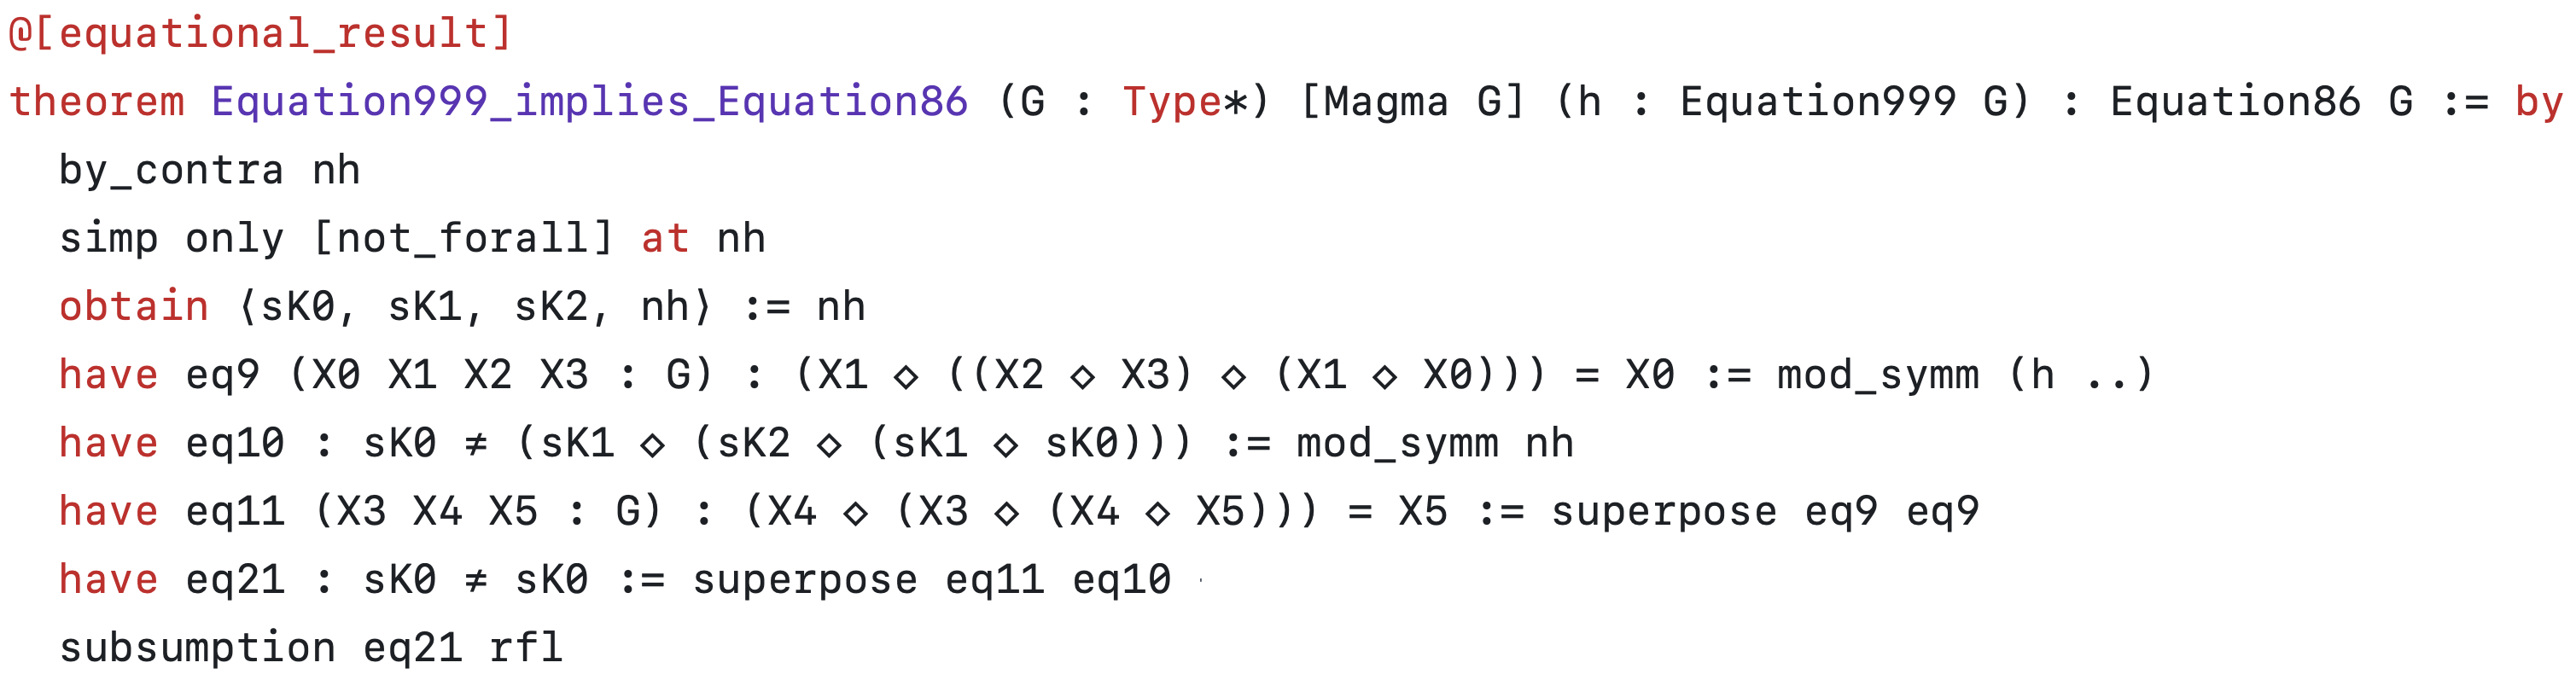
\includegraphics[width=\textwidth]{vampire-example.png}
  \caption{Example of a proof reconstructed from output of \emph{Vampire}. Note how the proof proceeds by contradiction and uses the \texttt{superpose} and \texttt{subsumption} steps implemented in \emph{Lean}.}
  \label{fig:vampire-example}
\end{figure}
\todo{Use listings or minted for this code block.}

\todo{Explain how Prover9 and Mace4 were used.}

For equational proofs from external provers, like \emph{MagmaEgg}, we also used a tailored version of reconstruction.
Specifically, the \emph{MagmaEgg} implementation turns \emph{explanations} \cite{nieuwenhuis2005proof} from \emph{egg} into \emph{Lean} proofs by simple applications of the defining properties of equality as shown in Figure~\ref{fig:magma-egg-example}.

\begin{figure}
  \centering
  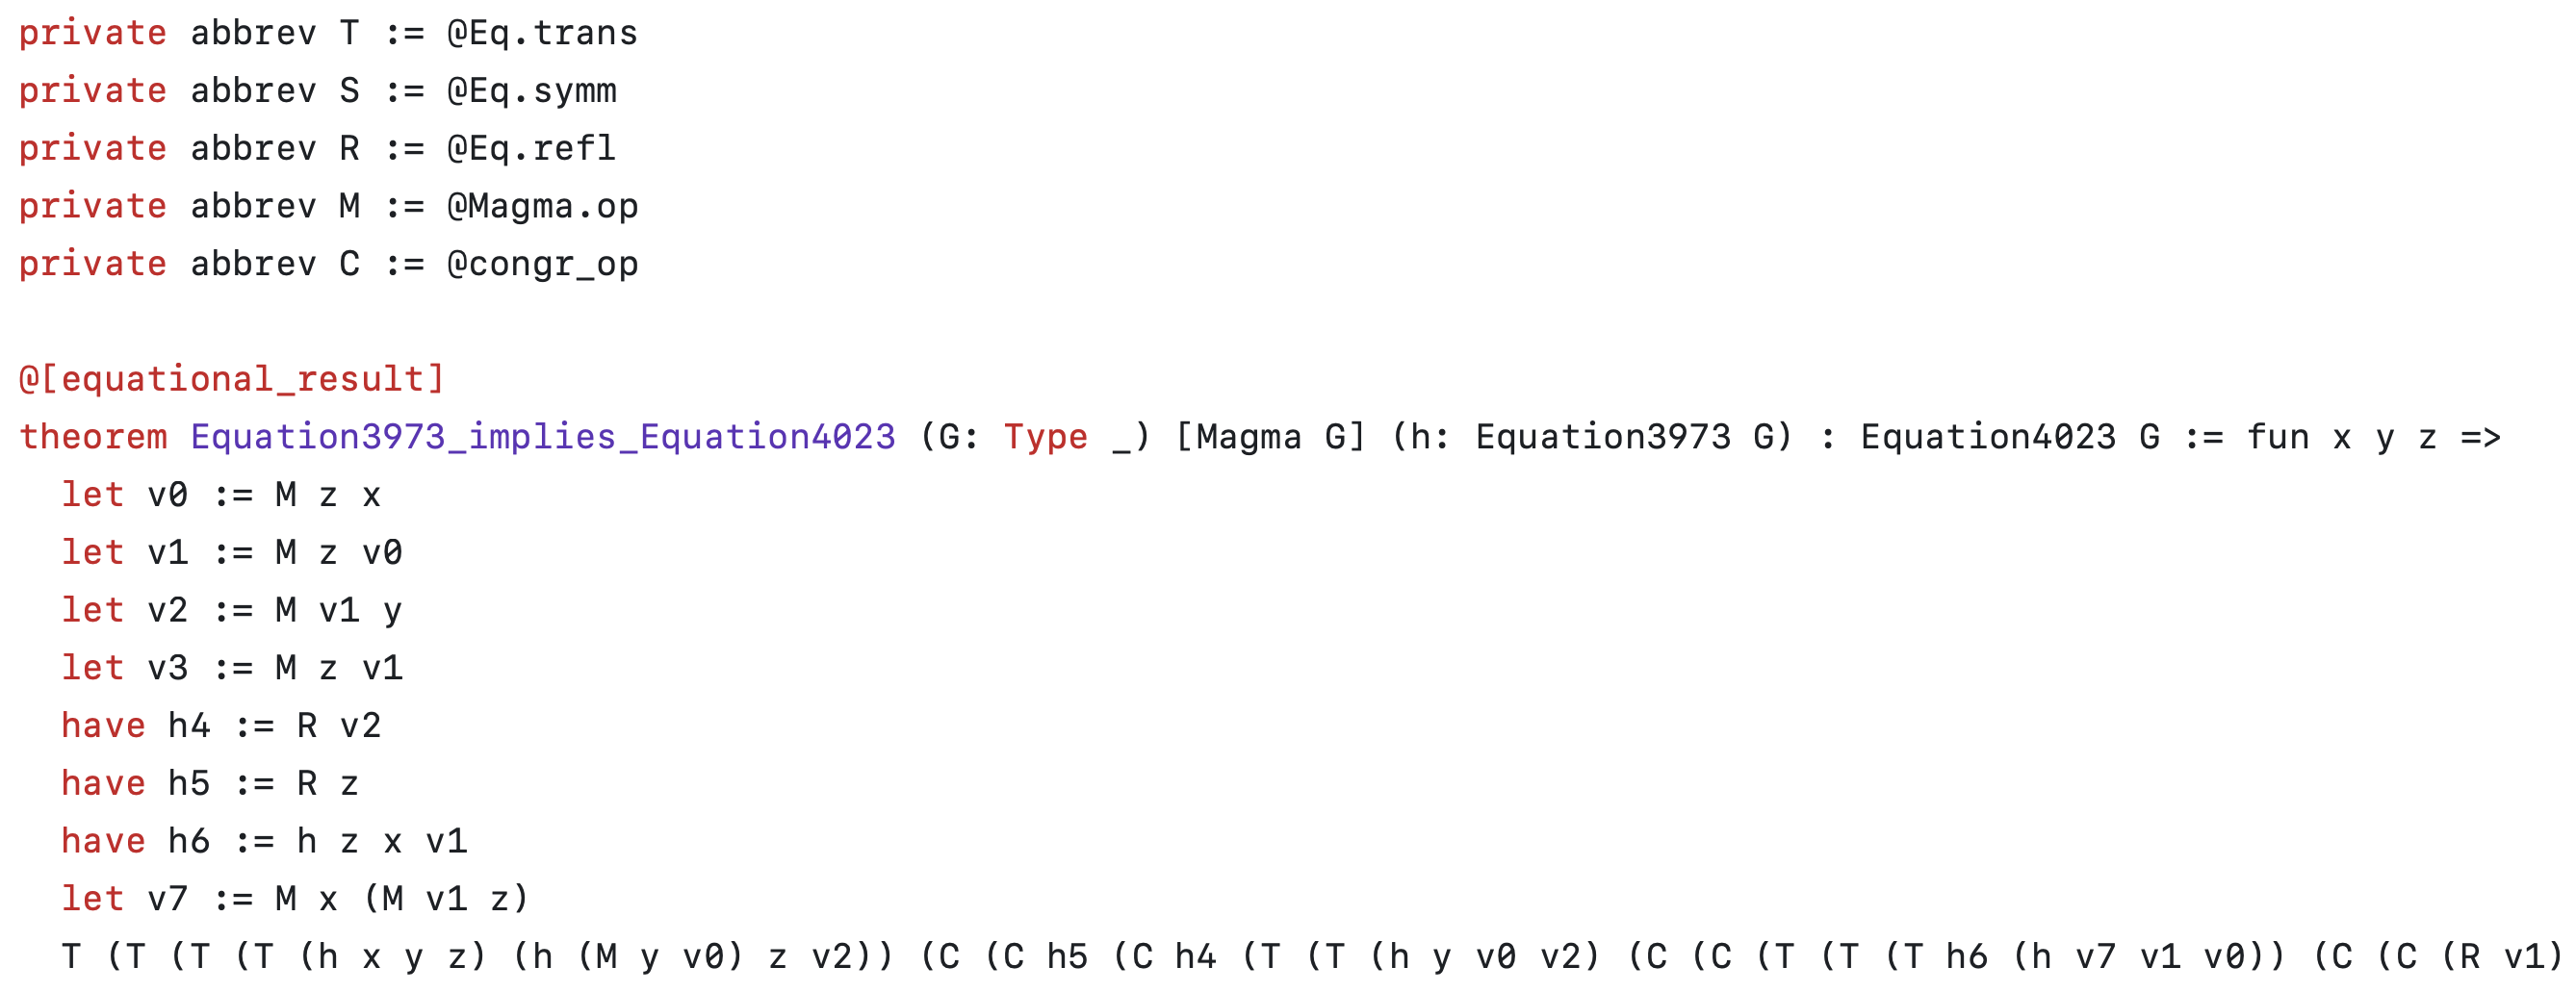
\includegraphics[width=\textwidth]{magma-egg-example.png}
  % SOURCE: https://github.com/teorth/equational_theories/blob/main/equational_theories/Generated/MagmaEgg/small/_005.lean
  \caption{Example of a proof reconstructed by \emph{MagmaEgg}. Note the proof only uses reflexivity, symmetry, transitivity, and congruence of equality.}
  \label{fig:magma-egg-example}
\end{figure}
\todo{Use listings or minted for this code block.}

In the case of the \texttt{egg} tactic, which also reconstructs proofs from \emph{egg} explanations, the proof could be converted into a more human-readable form by using the \texttt{calcify}\footnote{\url{https://github.com/nomeata/lean-calcify}} tactic, as shown in Figure~\ref{fig:egg-example}

\begin{figure}
  \centering
  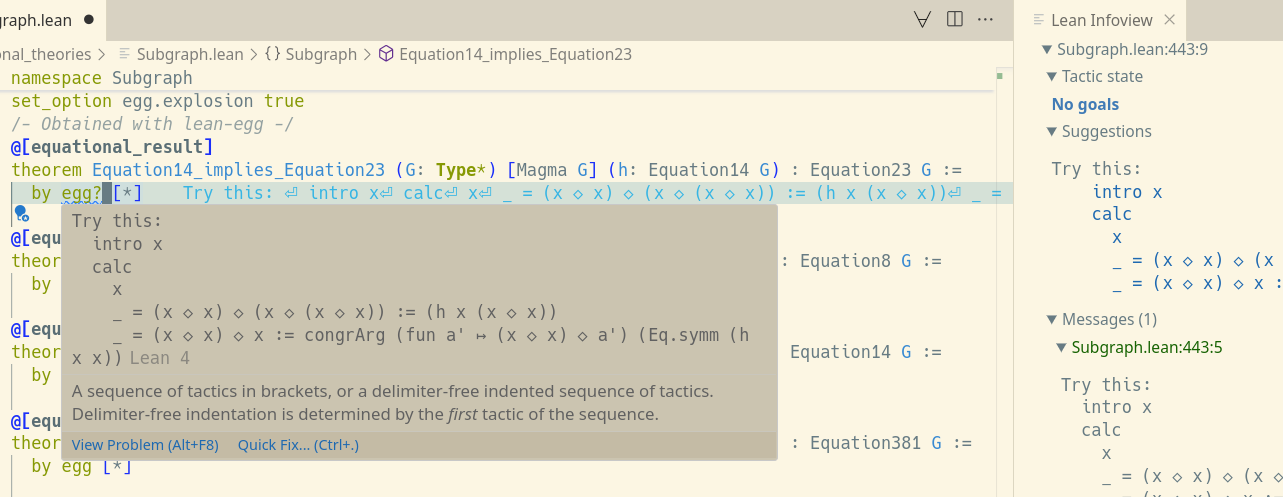
\includegraphics[width=\textwidth]{egg-example.png}
  \caption{Example of the \texttt{egg} tactic reconstructing a proof in human-readable form with the help of \texttt{calcify} (invoked by the special syntax \texttt{egg?}).}
  \label{fig:egg-example}
\end{figure}

\textbf{Semi-Automated Counterexample Guidance.}  Another use of ATPs has been in a semi-automatic fashion, to find counterexamples.
The general strategy was to use ATPs to find counterexamples to implications by building magmas iteratively.
If we want to build a counterexample to $l \vdash l'$, we want to construct a magma where $l$ holds but $l'$ does not.
In this method, we iteratively strengthen a construction with additional hypotheses, and use the ATP to check whether these hypotheses are not too strong (to imply $l'$) or unsound (to disallow $l$).

\TODO{this should also be expanded more, at least with references to some of the constructions in other chapters.}

While equational reasoning can also be used in a semi-automatic fashion to prove equations~\cite{DBLP:journals/pacmpl/KoehlerGBGTS24}, the positive implications in the main implication graph of project were all simple enough that we did not need a semi-automatic approach for them.

\TODO{discuss guided search in the finite implications or the Higman-Neumann work Jose Brox has done.}

\TODO{maybe add a screenshot here of the workflow of using a seed to find counterexamples with \emph{Prover9} or \emph{Vampire}?}

\subsection{Empirical Results}

Finally, we report some empirical results from use of ATPs for this project, in terms of performance.
This section is not intended to be a careful evaluation and benchmark comparison of the different ATPs; instead, we present our work here as a more informal ``field report'' documenting our experiences.
In particular, we do not draw firm conclusions about the overall capabilities\footnote{One reason for this is that different ATPs were deployed at different stages of the project.  In particular, the later ATP runs were performed in an environment when a large fraction of the implications had already been settled, and only a small remainder set was tested by our project.  The current set of ATP-generated formalized implications has also been subject to a number of reductions to optimize compilation time, so we would caution against reading too much into the raw number of such formalizations in the codebase.} of the different ATPs.
Rather, this serves as a use-case documenting the experience of (mostly) novice users.

\TODO{throw a couple of "benchmarking" tables for the same ATP with different parameters and for different ATPs, talk about some relative gains in time (changing parameters we saw a 500 times speedup on this particular problem), etc. This is knowledge I think we have gained to some extent, and certainly I would have been glad to receive this kind of hints before we started!''.  Then leave it as an interesting open problem to properly develop and measure benchmarks for ATPs based on this project.}

{\bf Any comparative study of semi-automated methods with fully automated ones? In principle, the semi-automated approach could be more automated using a script or "agent" to call various theorem provers. See \href{https://leanprover.zulipchat.com/#narrow/stream/458659-Equational/topic/A.20magma.20of.20order.20.3C.2013.20-.20for.20Equation2531.3F}{this discussion}}


{\bf See \href{https://leanprover.zulipchat.com/#narrow/channel/458659-Equational/topic/1516.20-.3E.20255/near/481547543}{this discussion} on the value of using different ATPs and setting run time parameters etc. at different values.}

{\bf What are the hardest implications to prove?  See \href{https://leanprover.zulipchat.com/#narrow/channel/458659-Equational/topic/What.20are.20the.20hardest.20positive.20implications.20for.20an.20ATP.3F}{this discussion}.}

\section{Implications for Finite Magmas}\label{austin-sec}

\TODO{Expand this sketch}

{\bf
Recap discussion from \url{https://leanprover.zulipchat.com/#narrow/channel/458659-Equational/topic/Austin.20pairs}
}

% \input{order5}
\section{Spectrum of equational laws}\label{spectrum-sec}

Given an equational law~$\Eq{n}$, one can ask for its spectrum, namely the set of cardinalities of its finite models.\footnote{The infinite spectrum is uninteresting (assuming the axiom of choice).  Let us show that if $\Eq{n}$ is not equivalent to the singleton law $\Eq{2}$ then it has models of all infinite cardinalities~$\kappa$.  The free magma on $\Eq{n}$ with $\kappa$ generators is such a model.  Indeed, the generators are distinct in this magma (otherwise $\Eq{n}$ would imply $\Eq{2}$) so its cardinal $\mu$ is at least $\kappa$.  Conversely, $\mu\leq\sum_T\kappa^{|T|}$ where the range sums over finite binary trees, and this sum is bounded above by $\aleph_0\cdot\kappa=\kappa$.}
The spectrum $\operatorname{Spec}(\Eq{n})$ is a multiplicative subset of $\mathbb{Z}_{>0}$ since the direct product of models is a model.
We focus here on the most basic question, that is, which laws (of order up to~$4$) have spectrum equal to $\mathbb{Z}_{>0}$?

Several extensions will be described in a separate publication: determining the spectrum and not only whether it is full; the spectrum of simple magmas or (sub)directly irreducible magmas; tracking multiplicity, namely counting (or bounding asymptotically) how many finite magmas exist of each size in the spectrum.  These detailed considerations reveal profound differences in how much an equational law constrains the magma operation, and may help organize the implication graph into different families.

An ATP run shows that $\num{1558}$ laws of order up to~$4$ have no model of size~$2$ and $\num{62}$ have a model of size~$2$ but none of size~$3$.  Pushing the search to higher model sizes does not resolve the question for any of the remaining $\num{3074}$ laws.  As we explain next, all of these laws actually have full spectrum.\footnote{Further investigations show that the lowest-numbered law with models of sizes $2$ and $3$ but not full spectrum is $\Eq{80887}$, namely $\x \formaleq \y \op (\y \op (\y \op (((\y \op \y) \op \x) \op \y)))$, of order~$6$.}


Our main tool by far to show that a law has full spectrum is to consider the carrying set $\mathbb{Z}/n\mathbb{Z}$, with a linear operation $x\op y = ax+by$ with $a,b\in\{-1,0,1\}$.  If the law holds for some choice of $a,b$ then the law has full spectrum.
\begin{itemize}
\item For $(a,b)=(0,0)$ the operation is the constant operation, which is a model of any law whose sides both have positive order.  Equivalently, these laws are consequences of the constant law $\Eq{41}$.
\item For $(a,b)=(1,0)$ the operation is a projection, which is a model of any law whose sides start with the same first variable, equivalently the consequences of $\Eq{4}$.  (The choice $(a,b)=(-1,0)$ is a model of fewer laws hence is not useful.)  Likewise $(a,b)=(0,1)$ shows that laws whose sides end with the same last variable (consequences of $\Eq{5}$) have full spectrum.
\item For $(a,b)=(1,-1)$ the operation is abelian group subtraction, characterized by Tarski's axiom $\Eq{543}$, which shows that any law implied by $\Eq{543}$ has full spectrum.  Likewise, backwards subtraction $(a,b)=(-1,1)$ provides models for $\Eq{1090}$ (equivalent to the dual of $\Eq{543}$) and its consequences.
\item The operation with $(a,b)=(1,1)$ cannot obey a law for all~$n$.
\item Finally, the operation $(a,b)=(-1,-1)$ is a model of some more laws, such as the semi-symmetric quasigroup law $\Eq{14}$ and totally symmetric quasigroup law $\Eq{492}$.
\end{itemize}
These considerations account for $\num{3068}$ laws, and there remains three dual pairs of laws to treat.  This is done through ad-hoc models: a piecewise linear model for $\Eq{1682}$ and its dual, and models whose operation table is mostly constant for the remaining laws $\Eq{1482}$, $\Eq{1523}$, and their duals.

Since a law implied by a full spectrum law has full spectrum itself, the implication graph reduces significantly the number of laws for which it is useful to formalize the full spectrum property.  Accounting for duality and implications, we found it sufficient to formalize the proof that $32$ laws have no magma of size~$2$ or none of size~$3$, and the explicit construction of magmas of all finite sizes for the $7$~laws $\Eq{4}$, $\Eq{41}$, $\Eq{492}$, $\Eq{543}$, $\Eq{1482}$, $\Eq{1523}$, and $\Eq{1682}$.  In conclusion, we prove that $\num{3074}$ laws ($65\%$) have full spectrum $\operatorname{Spec}(\Eq{n})=\mathbb{Z}_{>0}$ and $\num{1620}$ ($35\%$) do not (including $\num{1496}$ laws equivalent to $\Eq{2}$).  These percentages remain roughly stable at higher orders, with $60\%$ of laws of order up to $9$ having full spectrum, as will be reported elsewhere.

\section{Higman--Neumann laws}\label{higman-neumann}

\subsection{Describing groups as magmas}

The ETP is focused exclusively on magmas, which only feature a single (binary) operation.  Many mathematical structures traditionally defined using several operations can nevertheless be fully described as magmas with a well-chosen combined operation from which the whole structure can be reconstructed.  The first example is how Boolean algebras defined in terms of three operations $(\land,\lor,\lnot)$ were equivalently described in 1913 in terms of the Sheffer stroke $x\op y=\lnot(x\land y)$~\cite{sheffer1913set}.  Once such a single operation is found, a separate endeavor is to determine which laws it must obey to get the desired structure, and, in favorable cases find a single law that encapsulates the whole structure, or even find all equivalent laws of minimal order.  The earliest such example is Tarski's description of abelian groups in terms of subtraction $x\op y\coloneqq x+(-y)$ subject to a single axiom $\x \formaleq \y \op (\z \op (\x \op (\y \op \z)))$ \eqref{eq543} found in 1938~\cite{Tarski1938}.  It then took three decades~\cite{higman-neumann,Sholander01021959,Padmanabhan_1969} to sort out the full equivalence class of \eqref{eq543} among laws of order~$4$.  For Boolean algebras, a minimal-order single-law description was only found in~\cite{mccune_et_al}, nine decades after Sheffer's work.

We plan to report elsewhere on other examples such as modules over Eisenstein integers $\mathbb{Z}[\omega_3]$ or Gaussian integers $\mathbb{Z}[\omega_4]$, with $\omega_k$~a primitive $k$-th root of unity, which can be described by the operation $x \op y = x + \omega_k y$ subject to the order-$6$ laws \eqref{eq85914} and~\eqref{eq86082}, respectively.

Here, we describe the case of groups.  The binary operation~$*$, unary operation~$(\ )^{-1}$, and zeroary operation~$e$ (identity element), can be repackaged into a single division operation $x \op y = x*y^{-1}$, from which the original operations are easily reconstructed: for instance $x*y=x\op((y\op y)\op y)$.  A group equipped with division, called a Ward quasigroup, is a magma $(G, \op)$ obeying $\x \op \x \formaleq \y \op \y$ (unipotence law \eqref{eq40}), $\x \formaleq \x \op (\y \op \y)$ (right-unit squares law \eqref{eq11}), and a version of the associativity law dubbed the half-group law, $\x \op \y = (\x \op \z) \op (\y \op \z)$ \eqref{eq3737}, from which group axioms are easily derived.
These three laws are equivalent to a single law~\eqref{eq42323216} of order~$8$, found by Higman and Neumann~\cite{higman-neumann},
\[
\x \formaleq \y \op \Bigl(\bigl(((\y \op \y) \op \x) \op \z\bigr) \op \bigl(((\y \op \y) \op \y) \op \z\bigr)\Bigr) .
\]
McCune found two more laws equivalent to this one and of the same order \cite{mccune1993single}, \eqref{eq42302852} and \eqref{eq147976245}.  A natural question is to find all characterizations of Ward quasigroups (groups equipped with division) with minimal order.
Throughout our exploration, we used two criteria: the law must be obeyed by group division, and must fail for magmas that are not Ward quasigroups.

\subsection{Basic constraints}

There are $\num{298012537}$ laws of order up to~$8$, and running an ATP on all of them is too slow, so one needs efficient ways to filter them beforehand.  Let us begin with restrictions on the shape of any law equivalent to~\eqref{eq42323216}.
The law must take the form $\x\formaleq\dots$ as otherwise it would be obeyed by the constant operation on any set.
The law must be satisfied when evaluated with all variables set to the same element (say,~$1$) in the Ward quasigroup $\mathbb{Z}$ equipped with subtraction.  In particular the law must have even order.
This reduces from $\num{3470}$ shapes of order up to~$8$, down to just $548$~shapes.

Next come some restrictions on the variables.
The right-hand side must not start or end with the variable~$\x$ as otherwise the projection operations $x\op y=x$ or $x\op y=y$ would obey the law.
The law must have at least three variables: otherwise it is obeyed by division in any diassociative loop (such as a Moufang loop), namely a quasigroup with identity element and whose submagmas generated by pairs of elements are groups.
Each variable must appear an even number of times, so that the law holds in Boolean groups (abelian groups of exponent~$2$).
These basic constraints leave $54$, $\num{9000}$, and $\num{1841910}$~candidate laws of orders $4$, $6$, and~$8$, respectively, which can be efficiently enumerated since the conditions so far constrain the shape and rhyme scheme separately.

Imposing further that the law is obeyed by division in a free non-abelian group (with one generator per variable) reduces these numbers of laws to $0$, $59$, and $\num{5692}$ at these same orders.  All of the laws coming out of these filters are consequences of the Higman--Neumann law~\eqref{eq42323216} and one must determine which of these candidates imply that law.

\subsection{Using automated theorem provers.}

We repeatedly whittled down the list of candidates by accumulating a collection of finite countermodels, namely magmas that satisfy a candidate law while violating one of the laws \eqref{eq11}, \eqref{eq40} and~\eqref{eq3737} characterizing Ward quasigroups.  Automated searches of small magmas (of size $\leq 8$) with \emph{Mace4} or \emph{Vampire} gave many countermodels.  A second source was linear models $x \op y = ax+by$ on $\mathbb{Z}/n\mathbb{Z}$ with $(a,b)\neq(1,n-1)$: the largest one we used is $x \op y = 261x + 33y \bmod 307$ to rule out the candidate law $\Eq{68185620}$, $\x \formaleq (\y \op \y) \op (\y \op ((\x \op (\z \op \y)) \op ((\x \op \x) \op \z)))$.  Finally, we introduced some models that are ``almost'' Ward quasigroups: the 7-element smallest non-associative inverse loop (equipped with division), the 10-element smallest non-associative Steiner loop (commutative loop in which divisions coincide with multiplication), and the 16-element Moufang loop of unit octonions over~$\mathbb{Z}$.  Altogether, these steps eliminated all candidates of order less than~$8$, and left only $213$ laws of order~$8$ that could be equivalent to~\eqref{eq42323216}.

We showed the implication $\E\vdash\Eq{42323216}$ for $179$ candidate laws~$\E$ using the ATP \emph{Prover9}.  For equations of this order, the ATP computation times increase significantly compared to order 4 laws, with some proofs taking 20 times longer than checking with \emph{Prover9} all $\num{8178279}$ positive implications of the main project.  The choices of parameters bounding the ATP search (such as the parameter \texttt{max\_weight} limiting clause complexity in \emph{Prover9}) were particularly crucial, with different values being optimal in different proofs.  Another important speed-up was obtained by seeking proofs of a simple property such as \eqref{eq11}, \eqref{eq40}, \eqref{eq3737}, or injectivity/surjectivity of left or right multiplications, then seeking proofs that the candidate law together with that property implies some other property, and so on, until proving all three laws characterizing Ward quasigroups.  The reverse approach also proved useful, namely find which property would allow the proof to succeed, then seek a proof of that property from the candidate law.  Law \eqref{eq102744082} was a particularly difficult instance: together with injectivity of right multiplications it easily implies the Higman--Neumann law, but the proof that \eqref{eq102744082} does imply injectivity took 10 hours to obtain.

We showed the finite implication $\E\vdashfin\Eq{42323216}$ for $21$~laws~$\E$ (among the $34$ remaining candidates), which means that the law $\E$ characterizes Ward quasigroups among finite magmas.  Let us illustrate the proof technique for $\x \formaleq (\y \op \y) \op (\y \op ((\x \op \z) \op (((\x \op \x) \op \y) \op \z)))$ \eqref{eq67953597}.  In a finite magma, one gets $x = L_{y\op y} \circ L_y \circ f_{y,z}(x)$ where $L$ denotes left multiplication and $f_{y,z}(x) = (x\op z) \op (((x \op x) \op y) \op z)$.  Finiteness implies that the composition of several functions can only be a bijection if all of them are bijection, thus left multiplications are bijective.  By selecting $y=L_{x\op x}^{-1}(w)$ one gets that $(x\op z)\op (w\op z)$ equals the $z$-independent expression $L_y^{-1} \circ L_{y\op y}^{-1}(x)$.  Taking $w=x$ yields that the square of $L_x(z)$ is $z$-independent, hence (by surjectivity of~$L_x$) all squares are equal.  A routine ATP run then concludes.
While the resulting proofs of finite implications are relatively short and have been successfully ported to \emph{Lean}, our automated search involved thousands of \emph{Vampire} runs.
Indeed, rather than the condition that a bijective composition implies bijectivity of its constituents, we had to use the more concrete property that injectivity is equivalent to surjectivity for various collection of specific functions $f\colon M\to M$ such as left or right multiplications, cubing, etc.\@, with a brute-force search over which functions to include in a given run.

Altogether, out of the $\num{298012537}$ laws of order up to~$8$, we found $179$ laws characterizing Ward quasigroups, $21$~characterizing them among finite magmas but perhaps not infinite ones, and $13$~candidates for which we have neither a counterexample nor a proof even for finite magmas.  Regardless of these uncertainties, the lowest-numbered law characterizing Ward quasigroups is McCune's law~\eqref{eq42302852}.  These results have \emph{not} been formalized in \emph{Lean}.

% 179 laws equivalent to the Higman--Neumann law: [42302852, 42302946, 42303162, 42323122, 42323216, 42323432, 42358580, 42358644, 42358811, 42358978, 42359145, 42359357, 44390541, 44410811, 44445959, 44446330, 44446361, 44446423, 44446458, 48217845, 48272890, 48273536, 48273682, 48273989, 58075659, 58095929, 58130179, 58130628, 58131718, 58131745, 58131773, 67953907, 67957244, 67957681, 67957848, 67958015, 67958182, 67958395, 68185686, 68189095, 68189903, 68189965, 68189996, 68190031, 68653446, 68653573, 68653719, 68653865, 68654183, 69577454, 69580266, 69581164, 69581778, 69581832, 69581861, 70970200, 70973958, 70978107, 70978190, 71557731, 71558182, 73169267, 73173204, 73179688, 73180065, 73180415, 73180442, 73180499, 73186121, 73198517, 73210913, 73231927, 73231955, 73287395, 73290663, 73294472, 73298835, 73299635, 73300470, 75621653, 75646445, 75667496, 75667651, 89176740, 89178865, 89180041, 89182328, 89184615, 89188156, 89188210, 89188239, 90252914, 90263396, 90271271, 90276806, 90290863, 102398486, 102401815, 102402260, 102402594, 102402761, 102402975, 102744082, 102747350, 102751108, 102755257, 102755340, 105877516, 105877732, 105881069, 105881506, 105881673, 105881840, 105882007, 105882220, 110519688, 110520065, 110520442, 110520510, 110520844, 110521225, 113068011, 113071420, 113072228, 113072290, 113072321, 113072356, 121882187, 121884995, 121885893, 121886499, 121886561, 121886596, 122350887, 122355028, 122355125, 122696042, 122699868, 122704164, 122704989, 122705861, 125133271, 125133544, 125133690, 125134008, 126410158, 126413906, 126414357, 129417142, 129421079, 129427940, 129428317, 129428374, 147976245, 147976527, 147979351, 147979800, 147980249, 147980899, 147980911, 147980917, 149944702, 149948457, 149948639, 149955111, 149955500, 149955907, 149955913, 149955925, 157254554, 157257366, 157258264, 157258961, 163863870, 163867138, 163869006, 163870947, 163875310, 163876945]
% 21 laws equivalent for finite magmas: [48273390, 67953597, 67953691, 71553983, 73173015, 73285871, 73288447, 73292531, 89177565, 90206751, 90209038, 90214894, 90265736, 105877422, 129416953, 129420890, 129427563, 129428290, 157258878, 157258932, 163876110]
% 13 remaining candidates: [48217520, 48217671, 58095440, 73169078, 73169229, 102743259, 102745815, 102749116, 113067945, 113071354, 121884950, 122693826, 122697948]

\section{AI and Machine Learning Contributions}\label{ml-sec}

As discussed in \Cref{automated-sec}, the ETP made extensive use of automated theorem provers in completing the primary goal of determining and then formalizing all the implications between the specified equational laws.  In contrast, we were only able to utilize modern large language models (LLMs) in a fairly limited fashion.  Such models were useful in writing initial code for graphical user interfaces that we discuss further in \Cref{sec:gui-sec}, as well as performing some code autocompletion (using tools such as \emph{Github Copilot}) when formalizing an informal proof in \emph{Lean}.  In one instance, \emph{ChatGPT} was used\footnote{\url{https://chatgpt.com/share/670ce7db-8a44-800d-a5dc-8462c12eca3b}} to guess a complete rewriting system for the law $\x \op ((y \op y) \op \z) \formaleq x \op y$ \eqref{eq1659} which could then be formally verified, thus resolving all implications from this equation. However, in most of the difficult implications that resisted automated approaches, we found that LLMs did not provide useful suggestions beyond what the human participants could already propose.

On the other hand, we found that machine learning (ML) methods showed some promise of being able to heuristically predict the truth value of portions of the implication graph; we shall now discuss a convolutional neural network approach.\footnote{For some discussion of other ML experiments performed during the project, see \url{https://leanprover.zulipchat.com/\#narrow/channel/458659-Equational/topic/Machine.20learning.2C.20first.20results} for a (vectorized) transformer neural network approach, and \url{https://leanprover.zulipchat.com/#narrow/channel/458659-Equational/topic/Graph.20ML.3A.20Directed.20link.20prediction.20on.20the.20implication.20graph} for directed link prediction on the implication graph using Graph Neural Network (GNN) autoencoders.}

\subsection{Convolutional neural network model for the implication graph}

To model the implication graph, we used a convolutional neural network (CNN). For each pair of equations $(p,q)$, the input of the CNN consisted of a character-level tokenization (no vectorization) of the two equations, and the output of the CNN was a yes/no label depending on whether $p$ implies $q$. The CNN processed the input data using a 5-layer architecture, each layer composed of a 1-D convolution, followed by batch normalization and rectified linear unit activation functions (\cite{Goodfellow-et-al-2016}). After the last convolutional layer, a flattening layer and a softmax activation function were used to obtain the output of the network, i.e., the prediction of the implication for the input pair of equations. Note that we trained our models with the 16/10/2024 version of the (infinite) implication graph, for which 362 of the hardest implications (less than 0.002\% of the total) were still unknown.

\smallskip

Prior to training the CNN, we divided the data into training (60\%),validation (20\%), and test (20\%) subsets. The CNN was implemented in TensorFlow 2.9.0 (\cite{tensorflow2015-whitepaper}) and trained on an NVIDIA 3080 Ti GPU with the following configuration: the binary cross-entropy as the loss function to minimize, the Adam method with an initial learning rate of $10^{-3}$ for the adjustment of network weights, a batch size of 1024 with random shuffling, a learning rate reduction by a factor of 2 after 15 epochs without improvement in the validation loss, and early stopping if no improvement occurred for 40 epochs, being the model with the lowest validation loss retained as the final CNN.
The final CNN was evaluated on the test set, reaching a prediction accuracy of 99.7\%, which means that the model misclassified around 66k of the 22 million implications. Since this accuracy was somewhat surprising for such a small and “simple” model, as a control we generated a random label (yes/no) for each pair of equations, then trained the CNN on this data with 60\%/20\%/20\% training/validation/test percentages, resulting in a 49.99\% accuracy, as expected from a nonbiased model.

\smallskip

It could be the case that the high accuracy of our CNN model was mostly due to it learning the transitivity of the implication relation, as opposed to it discovering patterns in the identities. To clarify this point, it was proposed to train our CNN model either on a random poset or on the equational poset with vertices and labels permuted, and check whether a similar accuracy was achieved. This experiment has not been performed yet.

\smallskip

In any case, since there are around 600k explicit implications from which the rest can be derived by transitivity (2.7\% of the total), if the CNN was learning transitivity it should perform well with a really small training dataset. Accordingly, we trained and assessed a CNN model with a 5\%/5\%/90\% training/validation/test proportion, with a resulting 99.6\% accuracy on test (the process finishing in under 20 minutes). But the high accuracy is maintained with even smaller training datasets, as evidenced in the following table:
\begin{table}[h]
\centering
\begin{tabular}{|c|c|}
\hline
  % after \\: \hline or \cline{col1-col2} \cline{col3-col4} ...
  \textbf{Training/validation/test proportion (\%)} & \textbf{Prediction accuracy (\%)} \\\hline\hline
  60/20/20 & 99.7 \\\hline
  5/5/90 & 99.6 \\\hline
  1/1/98 & 99.3 \\\hline
  0.5/0.5/99 & 98.9 \\\hline
  0.1/0.1/99.8 & 92.2 \\
  \hline
\end{tabular}
\caption{Prediction accuracy as function of size of training set}
\end{table}

\noindent Since these training datasets were sensibly smaller than the subset of explicit implications, and were not carefully chosen from the poset extremes but taken randomly, we can conclude that even if the CNN was learning transitivity, probably this alone is not enough to explain the high accuracy achieved by the CNN model.

\smallskip

Since sometimes machine learning is announced as a form of data compression, let us now comment on the level of data compression achieved by our CNN model. In the table below we compare the sizes of three different encodings of the implication graph: a) As the simplest approach, we can encode the full implication graph in one file as labelled pairs of equations of the form ($p$, $q$, yes/no). b) On the other extreme, we can encode it as a bit table not containing neither the explicit equation expressions nor their numbers, but just a 1/0 label for each point with coordinates ($p$,$q$), together with a table mapping each number to its corresponding equation expression and a small script to recover the file in a). c) Finally, we can encode it in the complete files of the CNN model produced by TensorFlow 2.9.0. In addition, we can either consider these files in their raw form, or we can highly (but losslessly) compress them to achieve a rough comparison of their actual information content; accordingly, in the table below we also include the sizes of the encoding models when compressed with 7-zip LZMA2 ultra compression with a 1536MB dictionary size and a 273 word size.

\begin{table}[h]
\centering
\begin{tabular}{|c|c|c|}
  \hline
  % after \\: \hline or \cline{col1-col2} \cline{col3-col4} ...
  \textbf{Encoding model} & \textbf{Uncompressed size} & \textbf{Compressed size} \\\hline\hline
  Labelled pairs of equations & 1.5GB & 9MB \\\hline
  Bit table & 42MB & 40KB \\\hline
  CNN (99.7\% accuracy) & 1.34MB & 700KB \\
  \hline
\end{tabular}
\caption{Sizes of different encodings for the implication graph}
\end{table}

\smallskip

\noindent As we see, the information in the CNN model is more than 13 times less than in the labelled pairs model, while it is more than 18 times that of the bit table model. We also note that the CNN model in its raw form is already quite incompressible, and more than 30 times smaller than the raw bit table.

\smallskip

Lastly, also take into consideration that our CNN model does not only encode the implication graph up to order 4 (with 0.03\% of noise), but a priori may also be able to predict it for higher orders with a significant accuracy. Thus it could be used to guide and speed up the determination of the implication graph up to order 5, by letting ATPs focus first on the CNN’s predicted status of the studied implication.

\section{User Interfaces}\label{gui-sec}

A number of custom web applications were developed as part of the ETP. While many past Lean formalization projects have primarily relied on the Lean blueprint tool to organize tasks and track progress, the large volume of (transitive) implications tracked by the ETP, along with the research-oriented nature of the project, necessitated the development of custom tools to complement the blueprint tool. These web applications also made information more accessible to project participants and other interested parties, including those unfamiliar with Lean or the custom software developed for the project. The project features four primary interfaces:

\begin{enumerate}
  \item The \textbf{ETP dashboard}\footnote{\url{https://teorth.github.io/equational_theories/dashboard/}} displays the high-level overview of the project: the total number of resolved, conjectured, and unknown implications for the general and finite implication graphs. The dashboard also includes links to other tools, data, and visualizations about the implication graphs.
  \item The \textbf{Equation Explorer}\footnote{\url{https://teorth.github.io/equational_theories/implications/}} is the primary tool to navigate the implication graph. For a given equation, it display its inbound and outbound implications, as well as other members of its equivalence class. The explorer allows navigating either the general or finite implication graphs. The explorer also features custom commentary for a given equation (when available), serving as a repository for information and links. It also links to Graphiti visualizations and an example of its smallest satisfying magma, if one exists. Figure~\ref{fig:screenshot-equation-explorer} shows an example view of the explorer.
  \item \textbf{Graphiti}\footnote{\url{https://teorth.github.io/equational_theories/graphiti/}} visualizes the implication graph as a Hasse diagram, where downward edges represent subset relationships, and upward edges represent implications. Equivalence classes are collapsed into single nodes for clarity. Graphiti supports search parameters to visualize specific subsets of the graph. It can also display the entire implication graph, though the complete graph is large and challenging to navigate. Figure~\ref{fig:854-like} is an example of a Graphiti visualization.
  \item The \textbf{Finite Magma Explorer}\footnote{\url{https://teorth.github.io/equational_theories/fme/}} tests which equations a given finite magma satisfies or fails to satisfy. Users input finite magmas as Cayley tables. The tool is aware of the finite implication graph, so if an input magma witnesses an unknown refutation, it notifies the user and provides instructions for contributing the result to the GitHub repository.
\end{enumerate}

\begin{figure}
  \centering
  \includegraphics[width=0.85\textwidth]{GUI-equation-explorer.png}
  \caption{An example of the information displayed by the Equation Explorer for a specific equation.}
  \label{fig:screenshot-equation-explorer}
\end{figure}

The data for these tools is extracted directly from the Lean-formalized proofs in the project's GitHub repository, ensuring it always faithfully reflects the current state of progress. Additionally, the data is automatically updated with each code change using continuous integration (CI), eliminating the need for manual updates.

\section{Data Management}

\TODO{expand this sketch}

Describe how data was handled during the project and how it will be managed going forward.

\section{Conclusions and Future Directions}

This project successfully demonstrated that large-scale explorations of a space of mathematical statements - in this case, the implications or non-implications between selected equational laws - can be crowdsourced using modern collaboration platforms and proof assistants.  No single tool or method was able to study the entirety of this space, and many informal proofs generated contained non-trivial errors; but there were multiple techniques that could treat significant portions of the space, and through a collaborative effort combined with the proof validation provided by \emph{Lean}, one could synthesize these partial and fallible contributions into a complete and validated description of the entire implication graph.  While this particular graph was a comparatively simple structure to analyze, we believe that this paradigm could also serve as a model for future projects devoted to exploring more sophisticated large-scale mathematical structures.

Several factors appeared to be helpful in ensuring the success of the project, including the following:
\begin{itemize}
\item \textbf{A clearly stated primary goal, with an end condition and precise numerical metrics to measure partial completion.}  From the outset, there was a specific goal to attain, namely to completely determine and then formalize the implication graph on the original set of $4694$ laws.  Progress towards that goal could be measured by a number of metrics, such as the number of implications that were conjectured but unformalized, or not conjectured at all.   Such metrics allowed participants to see how partial contributions, such as formalizing a certain subset of implications, advanced the project directly towards its primary goal.  This is not to say that all activity was devoted solely towards this primary goal, but it did provide a coherent focus to help guide and motivate other secondary activities.
\item \textbf{A highly modular project}.  It was possible for any given coauthor to work on a small subset of implications and focus on a single proof technique, without needing to understand or rely upon other contributions to the project.  This allowed the work to be both parallelized and decentralized; many contributors launched their own investigations broadly within the framework of the project, without needing centralized approval or coordination.
\item \textbf{Low levels of required mathematical and formal prerequisites}.  The problems considered in the project did not require advanced mathematical knowledge (beyond a general familiarity with abstract algebra), nor a sophisticated understanding of formal proof assistants.  This permitted contributions from a broad spectrum of participants, including those without a graduate mathematical training, as well as mathematicians with no experience in proof formalization.  At a technical level, it also meant that formalization of proofs into \emph{Lean} could be done immediately once certain base definitions (such as \texttt{Magma}) were constructed.  This can be compared for instance with the recent formalization of the Polynomial Freiman--Ruzsa conjecture\footnote{\url{https://github.com/teorth/pfr}}, in which significant effort was expended in the first few days to settle on a suitable framework to formalize the mathematics of Shannon entropy.  While some more sophisticated formal structures (such as the syntactic description of laws as pairs of words in a \texttt{FreeMagma}) were later introduced in the project, it was relatively straightforward to refactor previously written code to be compatible with these structures as they were incorporated into the project.
\item \textbf{Variable levels of difficulty, and the amenability to partial progress.}  Traditional mathematics projects generally involve a small number of extremely hard problems, with incomplete progress on these problems being difficult to convert into clean partial results.  In contrast, the ETP studied a large number of problems with a very broad range of difficulty, so that even if a given proof strategy did not work for a given implication, it could be the case that there was some class of easier implications for which the strategy was successful.  This allowed for a means to validate such ideas, and allowed the project to build up a useful and diverse toolbox of proof techniques which became increasingly necessary to handle the final and most difficult implications in the project.  It also created a dynamic in which the project initially focused on easy techniques to resolve a significant fraction of the implications, gradually transitioning into more sophisticated methods that focused on a much smaller number of outstanding implications that had proven resistant (or even ``immune'') to all easier approaches.
\item \textbf{Centralized and standardized platforms for discussion, project management, and validation.}  While the project was decentralized at the level of the participant, there was a centralized location (a channel\footnote{\url{https://leanprover.zulipchat.com/\#narrow/channel/458659-Equational}} on the Lean Zulip) to discuss all aspects of the project, as well as a centralized repository\footnote{\url{https://github.com/teorth/equational_theories}} to track all contributions and outstanding issues, a centralized blueprint\footnote{\url{https://teorth.github.io/equational_theories/blueprint/}} to describe technical details of proofs to be formalized, and a single formal language (\emph{Lean}) to validate all contributions. A significant portion of the activity in the early stages of the project was devoted to setting out the standards and workflows for handling both the discussion and the contributions, in particular setting up a contributions page\footnote{\url{https://github.com/teorth/equational_theories/blob/main/CONTRIBUTING.md}} and adopting a code of conduct\footnote{\url{https://github.com/teorth/equational_theories/blob/main/CODE_OF_CONDUCT.md}}.  This gave some structure and predictability to what might otherwise be a chaotic effort.
\item \textbf{Development of custom visualization tools.}  As discussed in \Cref{sec:gui-sec}, several tools were developed (in part with AI assistance) to help visualize and navigate the implication graph while it was in a partial stage of development, allowing for participants to independently identify problems to work on, and to validate and use the contributions of other participants even before they were fully formalized.  For instance, a participant could propose a finite counterexample to an implication by posting a link to the magma in \emph{Finite Magma Explorer}, allowing for immediate validation of the counterexample, or use \emph{Equation Explorer} or \emph{Graphiti} to observe some interesting phenomenon in the implication graph that other participants could reproduce and study.
\item \textbf{Applicability of existing software tools.}  As described in \Cref{automated-sec}, many of the implications in the ETP were amenable to application of ``off-the-shelf'' automated theorem provers (ATPs); while some trial and error was needed to determine good choices of parameters, these tools could largely be applied directly to the project without extensive customization.  (However, the later transcription of ATP output into Lean was sometimes non-trivial.)
\item \textbf{Receptiveness to new techniques and tools.}  Crucially, the methods used to make progress on the project were not specified in advance, and contributions from participants with new ideas, techniques, or software tools that were not initially anticipated were welcomed.  For instance, the theory of canonizers (\Cref{canon-sec}) was not initially known to the first project participants, but was brought to the attention of the project by a later contributor.  Conversely, while there were hopes expressed early in the project that modern large language models (LLMs) could automatically generate many of the proofs required, it turned out in practice that other forms of automation, particularly ATPs, were significantly more effective at this task (at least if one restricted to publicly available LLMs), and the project largely moved away from the use of such LLMs (other than to help create the code for the visualization tools).
\end{itemize}

There are several mathematical and computational questions that could potentially be addressed in future work building upon the outcomes of ETP.  Here is a list of some possible such future directions.
\begin{enumerate}
  \item Does the law $\x \formaleq \y \op (\x \op ((\y \op \x) \op \y))$ (E677) imply $\x \formaleq ((\x \op \x) \op \x) \op \x$ (E255) for finite magmas? This is the last remaining implication (up to duality) for finite magmas to be resolved.  A number of partial results on this problem may be found at \url{https://teorth.github.io/equational_theories/blueprint/677-chapter.html}.
  \item Does the law $\x \formaleq \y \op (\y \op (\y \op (\x \op (\z \op \y))))$ (E5093) have any infinite models? In \cite{Kisielewicz2} it was shown that it has no finite models, but the infinite model case was left as an open question.
  \item The ETP focused on determining relations $\E \models \E'$ between one law and another.  Could the same methods also systematically determine more complex logical relations, such as $\E_1 \wedge \E_2 \models \E_3$, for all laws $\E_1,\E_2,\E_3$ in a specified set?
  \item A key feature of finite magmas $M$ is that they are surjunctive, in the sense that any definable map from $M$ to itself that is surjective, is also injective (or vice versa), where ``definable'' is with respect to the language of magmas.  Are there equational theories that admit surjunctive models, but yet do not have any finite models?
  \item Are there interesting examples of implications $\E_1 \models \E_2$ which are ``irreducible'' in the sense that there is no equational law $\E$ with $\E_1 \models \E \models \E_2$, other than those laws equivalent to either $\E_1$ or $\E_2$?
  \item How ``stable'' is a given law $\E$?  For instance, if a finite magma obeys a law $\E$ some proportion $1-\eps$ of the time, with $\eps$ small, can the magma be perturbed into one that obeys $\E$ exactly?  Related to this is the question of whether a law $\E$ is ``rigid'' or ``mutable'': is it possible to make a small number of modifications to a magma obeying $\E$ in a way that still preserves $\E$?  Such properties helped suggest whether certain magma construction techniques, such as modifying a base magma, were likely to be successful.
\end{enumerate}

\subsection{Miscellaneous remarks}

It is possible that the timing in which certain proof methods were introduced into the project created some opportunity costs.  For instance, by deploying automated theorem provers at an early stage, we might have settled some implications that had more interesting human-readable proofs that we missed.  Similarly, we developed some sophisticated theory for the equation \eqref{eq854}, such as \Cref{unique-factorization}, that is now superseded by finite counterexamples; but had the finite counterexamples been discovered first, we would not have found the theoretical arguments.  It may be productive for future work to revisit some portions of the implication graph and locate alternate proofs and methods.


\section*{Acknowledgments}

We are grateful to the many additional participants to the Equational Theories Project for their
numerous comments and encouragement, with particular thanks to  Stanley Burris, Edward van de Meent and David Roberts.


\appendix

\section{Numbering system}\label{numbering-app}

In this section we record the numbering conventions we use for equational laws.

For this formal definition we use the natural numbers $0,1,2,\dots$ to represent and order indeterminate variables; however, in the main text, we use the symbols $\x,\y,\z,\w,\uu,\vv,\mathrm{r},\mathrm{s},\mathrm{t}$ instead (and do not consider any laws with more than eight variables).

To define the ordering we use on equational laws, we first consider the case where there is a single indeterminate $\ast$.
We place a well-ordering on words $w,w'$ with a single indeterminate $\ast$ by declaring $w > w'$ if one of the following holds:
\begin{itemize}
    \item $w$ has a larger order than $w'$.
    \item $w = w_1 \op w_2$ and $w' = w'_1 \op w'_2$ have the same order $n \geq 1$ with $w_1 > w'_1$.
    \item $w = w_1 \op w_2$ and $w' = w'_1 \op w'_2$ have the same order $n \geq 1$ with $w_1 = w'_1$ and $w_2 > w'_2$.
\end{itemize}
Thus, for instance
$$ \ast < \ast \op \ast < \ast \op (\ast \op \ast) < (\ast \op \ast) \op \ast.$$

We similarly place a well-ordering on equational laws $w_1 \formaleq w_2$ with a single indeterminate $\ast$ by declaring $w_1 \formaleq w_2 > w'_1 \formaleq w'_2$ if one of the following holds:
as follows:
\begin{itemize}
\item  $w_1 \formaleq w_2$ has a longer order than $w'_1 \formaleq w'_2$.
\item If $w_1 \formaleq w_2$ has the same order as $w'_1 \formaleq w'_2$, and $w_1 > w'_1$.
\item If $w_1 \formaleq w_2$ has the same order as $w'_1 \formaleq w'_2$, $w_1 = w'_1$, and $w_2 > w'_2$.
\end{itemize}
Thus for instance
$$ (\ast \op \ast \formaleq \ast \op (\ast \op \ast)) < (\ast \op \ast \formaleq (\ast \op \ast) \op \ast).$$

Finally for equational laws with alphabet $\x,\y,\z,\w,\uu,\vv,\mathrm{r},\mathrm{s},\mathrm{t}$, define the \emph{shape} of that law to be the law formed by replacing all indeterminates with $\ast$; for instance, the shape of \eqref{eq4512}, $\x \op (\y \op \z) = (\x \op \y) \op \z$, is $\ast \op (\ast \op \ast) \formaleq (\ast \op \ast) \op \ast$.  We then place a well-ordering $w_1 \formaleq w_2$ with indeterminates $\x,\y,\z,\w,\uu,\vv,\mathrm{r},\mathrm{s},\mathrm{t}$ by declaring $w_1 \formaleq w_2 > w'_1 \formaleq w'_2$ if one of the following holds:
\begin{itemize}
\item The shape of $w_1 \formaleq w_2$ is greater than the shape of $w'_1 \formaleq w'_2$.
\item $w_1 \formaleq w_2$ and $w'_1 \formaleq w'_2$ have the same shape, and the string of variables appearing in $w_1 \formaleq w_2$ is lower in the lexicographical ordering (using $\x < \y < \z < \w < \uu < \vv < \mathrm{r} < \mathrm{s} < \mathrm{t}$) than the corresponding string for $w'_1 \formaleq w'_2$.
\end{itemize}
Thus for instance any law of shape $\ast \op \ast \formaleq \ast \op (\ast \op \ast)$ is lower than any law of shape
$\ast \op \ast \formaleq (\ast \op \ast) \op \ast$.  Among the laws of shape $\ast \op \ast \formaleq \ast \op (\ast \op \ast)$, the lowest is $\x \op \x \formaleq \x \op (\x \op \x)$, which is less than (say) $\x \op \x \formaleq \y \op (\y \op \y)$, which is in turn less than $\x \op \y \formaleq \x \op (\x \op \x)$.

We say that two equational laws are \emph{definitionally equivalent}\footnote{This can be distinguished from the weaker notion of \emph{propositional equivalence} (mutual entailment) used in the rest of the paper.} if one can be obtained from another by some combination of relabeling the variables and applying the symmetric law $w_1 \formaleq w_2 \iff w_2 \formaleq w_1$.  For instance, $(0 \op 1) \op 2 \formaleq 1$ is definitionally equivalent to $0 \formaleq (1 \op 0) \op 2$.  We then replace every equational law with their minimal element in their definitional equivalence class, which can be viewed as the \emph{normal form} for that law; for instance, the normal form of $(0 \op 1) \op 2 \formaleq 1$ would be $0 \formaleq (1 \op 0) \op 2$.  Finally, we eliminate any law of the form $w \formaleq w$ other than $0 \formaleq 0$.  We then number the remaining equations $\Eq{1}, \Eq{2}, \dots$.  For instance, $\Eq{1}$ is the trivial law $0 \formaleq 0$, $\Eq{2}$ is the constant law $0 \formaleq 1$, $\Eq{3}$ is the idempotent law $0 \formaleq 0 \op 0$, and so forth.  Lists and code for generating these equations, or the equation number attached to a given equation, can be found in the ETP repository.

The number of equations in this list of order $n=0,1,2,\dots$ is given by
$$ 2, 5, 39, 364, 4284, 57882, 888365, \dots$$
(\url{https://oeis.org/A376640}).  The number can be computed to be
$$ C_{n+1} B_{n+2}/2$$
if $n$ is odd, $2$ if $n=0$, and
$$ (C_{n+1} B_{n+2}+ C_{n/2}(2D_{n+2}-B_{n+2}))/2 - C_{n/2} B_{n/2+1}$$
if $n > 2$ is even, where $C_n, B_n$ are the Catalan and Bell numbers, and $D_n$ is the number of partitions of $[n]$ up to reflection, which for $n=0,1,2,\dots$ is
$$ 1, 1, 2, 4, 11, 32, 117, \dots$$
(\url{https://oeis.org/A103293}).  A proof of this claim can be found in the ETP blueprint.  In particular, there are $4694$ equations of order at most $4$.

Below we record some specific equations appearing in this paper, using the alphabet $\x$, $\y$, $\z$, $\w$, $\uu$, $\vv$ in place of $0$, $1$, $2$, $3$, $4$, $5$, $\dots$ for readability.
\begingroup\allowdisplaybreaks
\begin{align}
    \x &\formaleq \x & \hbox{(Trivial law)} \label{eq1}\tag{E1} \\
    \x &\formaleq \y & \hbox{(Singleton law)} \label{eq2}\tag{E2} \\
    \x &\formaleq \x \op \x & \hbox{(Idempotent law)} \label{eq3}\tag{E3} \\
    \x &\formaleq \x \op \y & \hbox{(Left-absorptive law)} \label{eq4}\tag{E4} \\
    \x &\formaleq \y \op \x & \hbox{(Right-absorptive law)} \label{eq5}\tag{E5} \\
    \x &\formaleq \x \op (\y \op \x) \label{eq10}\tag{E10} \\
    \x &\formaleq \x \op (\y \op \y) & \hbox{(Right-unit squares law)} \label{eq11}\tag{E11} \\
    \x &\formaleq (\x \op \x) \op \x \label{eq23}\tag{E23} \\
    \x \op \x &\formaleq \y \op \y & \hbox{(Unipotence law)} \label{eq40}\tag{E40} \\
    \x \op \x &\formaleq \y \op \z & \hbox{(Constant law)} \label{eq41}\tag{E41} \\
    \x \op \y &\formaleq \y \op \x & \hbox{(Commutative law)} \label{eq43}\tag{E43} \\
    \x \op \y &\formaleq \z \op \w & \hbox{(Constant law)} \label{eq46}\tag{E46} \\
    \x &\formaleq \x \op (\x \op (\x \op \x)) \label{eq47}\tag{E47} \\
    \x &\formaleq \y \op (\y \op (\x \op \y))  \label{eq73}\tag{E73} \\
    \x &\formaleq (\x \op \x) \op (\x \op \x) \label{eq151}\tag{E151} \\
    \x &\formaleq (\y \op \x) \op (\x \op \z) & \hbox{(Central groupoid law)} \label{eq168}\tag{E168} \\
    \x &\formaleq (\x \op (\x \op \y)) \op \y \label{eq206}\tag{E206} \\
    \x &\formaleq ((\x \op \x) \op \x) \op \x \label{eq255}\tag{E255} \\
    \x \op \y &\formaleq \x \op (\y \op \z) & \hbox{(Right reduction law)} \label{eq327}\tag{E327} \\
    \x \op \y &\formaleq (\x \op \y) \op \y & \hbox{(Right idempotence law)} \label{eq378}\tag{E378} \\
    \x \op \y &\formaleq (\z \op \x) \op \y & \hbox{(Left reduction law)} \label{eq395}\tag{E395} \\
    \x &\formaleq \x \op (\x \op (\x \op (\y \op \x))) \label{eq413}\tag{E413} \\
    \x &\formaleq \y \op (\z \op (\x \op (\y \op \z))) & \hbox{(Tarski's axiom)} \label{eq543}\tag{E543} \\
    \x &\formaleq \y \op (\x \op ((\y \op \x) \op \y)) & \hbox{(Last open implication)} \label{eq677}\tag{E677} \\
    \x &\formaleq \x \op ((\x \op \x) \op (\x \op \x)) \label{eq817}\tag{E817} \\
    \x &\formaleq \x \op ((\y \op \z) \op (\x \op \z)) \label{eq854}\tag{E854}\\
    \x &\formaleq \x \op ((\y \op (\y \op \x)) \op \x) \label{eq1045}\tag{E1045} \\
    \x &\formaleq \x \op ((\y \op (\z \op \x)) \op \x) \label{eq1055}\tag{E1055} \\
    \x &\formaleq \y \op ((\y \op (\x \op \x)) \op \y) \label{eq1110}\tag{E1110} \\
    \x &\formaleq \y \op ((\y \op (\x \op \z)) \op \z) \label{eq1117}\tag{E1117} \\
    \x &\formaleq \y \op (((\x \op \y) \op \x) \op \y) \label{eq1286}\tag{E1286} \\
    \x &\formaleq (\y \op \x) \op (\x \op (\z \op \y)) & \hbox{(Weak central groupoids)}\label{eq1485}\tag{E1485} \\
    \x &\formaleq (\y \op \z) \op (\y \op (\x \op \z)) & \hbox{(Boolean groups)} \label{eq1571}\tag{E1571} \\
    \x &\formaleq (\x \op \x) \op ((\x \op \x) \op \x) \label{eq1629}\tag{E1629} \\
    \x &\formaleq (\x \op \y) \op ((\x \op \y) \op \y) \label{eq1648}\tag{E1648} \\
    \x &\formaleq (\x \op \y) \op ((\y \op \y) \op \z) \label{eq1659}\tag{E1659} \\
    \x &\formaleq (\y \op \x) \op ((\x \op \z) \op \z) & \hbox{(Equivalent to~\eqref{eq2})} \label{eq1689}\tag{E1689} \\
    \x &\formaleq (\y \op \y) \op ((\y \op \x) \op \y) \label{eq1729}\tag{E1729} \\
    \x &\formaleq (\y \op (\x \op (\y \op \x))) \op \y \label{eq2301}\tag{E2301} \\
        \x &\formaleq (\x \op ((\x \op \x) \op \x)) \op \x \label{eq2441}\tag{E2441} \\
        \x &\formaleq ((\y \op (\x \op \y)) \op \x) \op \y & \hbox{(Dual of \eqref{eq677})} \label{eq2910}\tag{E2910} \\
        \x \op \y &\formaleq \x \op (\y \op (\x \op \y)) \label{eq3316}\tag{E3316} \\
        \x \op \y &\formaleq (\x \op \z) \op (\y \op \z) \label{eq3737}\tag{E3737} \\
        \x \op \y &\formaleq (\x \op (\y \op \x)) \op \y \label{eq3925}\tag{E3925} \\
        \x \op (\y \op \x) &\formaleq \x \op (\y \op \z) \label{eq4315}\tag{E4315} \\
        \x \op (\x \op \x) &\formaleq (\x \op \x) \op \x & \hbox{(Cube-associativity law)} \label{eq4380}\tag{E4380} \\
        \x \op (\y \op \y) &\formaleq (\y \op \y) \op \x & \hbox{(Central squares law)} \label{eq4482}\tag{E4482} \\
        \x \op (\y \op \z) &\formaleq (\x \op \y) \op \z & \hbox{(Associative law)} \label{eq4512}\tag{E4512} \\
        \x \op (\y \op \z) &\formaleq (\y \op \z) \op \x & \hbox{(Central products law)} \label{eq4531}\tag{E4531} \\
        \x &\formaleq \y \op (\y \op (\y \op (\x \op (\z \op \y)))) \label{eq5093}\tag{E5093} \\
        \x &\formaleq \y \op (\z \op ((\y \op \x) \op (\z \op (\y \op \z)))) & \hbox{(Eisenstein modules)} \label{eq85914} \tag{E85914} \\
        \x &\formaleq \y \op (\z \op ((\y \op \z) \op (\w \op (\x \op \w)))) & \hbox{(Gaussian modules)} \label{eq86082} \tag{E86082} \\
        \x &\formaleq (\y \op ((\x \op \y) \op \y)) \op (\x \op (\z \op \y)) & \hbox{(Sheffer stroke)} \label{eq345169}\tag{E345169}
\end{align}
We also list some order-$8$ characterizations of group division relevant for \Cref{higman-neumann}.
\begin{align}
        \x &\formaleq \y \op ((((\x \op \x) \op \x) \op \z) \op (((\x \op \x) \op \y) \op \z)) & \hbox{(McCune law)} \label{eq42302852}\tag{E42302852} \\
        \x &\formaleq \y \op ((((\x \op \x) \op \x) \op \z) \op (((\y \op \y) \op \y) \op \z)) & \label{eq42302946}\tag{E42302946} \\
        \x &\formaleq \y \op ((((\y \op \y) \op \x) \op \z) \op (((\y \op \y) \op \y) \op \z)) & \hbox{(Higman--Neumann law)} \label{eq42323216}\tag{E42323216} \\
        \x &\formaleq (\y \op \y) \op (\y \op ((\x \op \z) \op (((\x \op \x) \op \y) \op \z))) & \hbox{(in finite magmas)} \label{eq67953597}\tag{E67953597} \\
        \x &\formaleq ((\y \op \y) \op \y) \op ((((\x \op \x) \op \x) \op \z) \op (\y \op \z)) & \label{eq89176740}\tag{E89176740} \\
        \x &\formaleq ((\y \op \y) \op ((\x \op \z) \op \x)) \op ((\z \op \w) \op (\x \op \w)) & \label{eq102744082}\tag{E102744082} \\
        \x &\formaleq ((\y \op \y) \op (\y \op (\x \op (((\y \op \y) \op \y) \op \z)))) \op \z & \hbox{(McCune law)} \label{eq147976245}\tag{E147976245}
\end{align}
\endgroup

\section{Author Contributions}

In a \href{https://github.com/teorth/equational_theories/blob/main/paper/contributions.md}{companion document} to this paper, the contributions of each author of this paper to the ETP are described, following the standard CRediT categories\footnote{\url{https://credit.niso.org/}}.  Below are the affiliations and grant acknowledgments of individual participants.


\begin{itemize}
    \item Matthew Bolan: University of Toronto, matthew.bolan@mail.utoronto.ca
    \item Joachim Breitner: Lean FRO, mail@joachim-breitner.de, ORCID 0000-0003-3753-6821
    \item Jose Brox: IMUVA-Mathematics Research Institute, Universidad de Valladolid, josebrox@uva.es. Supported by a postdoctoral fellowship “Convocatoria 2021” funded by Universidad de Valladolid, and partially supported by grant PID2022-137283NB-C22 funded by MCIN/AEI/10.13039/501100011033 and ERDF “A way of making Europe”
    \item Mario Carneiro: ...
    \item Martin Dvorak: Institute of Science and Technology Austria, martin.dvorak@matfyz.cz
    \item Andr\'es Goens: University of Amsterdam, a.goens@uva.nl
    \item Aaron Hill: Unaffiliated, aa1ronham@gmail.com
    \item Harald Husum: harald.husum@gmail.com
    \item Hern\'an Ibarra Mejia: hernan@ibarramejia.com
    \item Zoltan A. Kocsis: University of New South Wales, z.kocsis@unsw.edu.au
    \item Bruno Le Floch: CNRS and Laboratoire de Physique Th\'eorique et Hautes \'Energies, Sorbonne Universit\'e, blefloch@lpthe.jussieu.fr
    \item Lorenzo Luccioli: University of Bologna, lorenzo.luccioli2@unibo.it
    \item Douglas McNeil: dsm054@gmail.com
    \item Alex Meiburg: Perimeter Institute for Theoretical Physics / University of Waterloo Institute for Quantum Computing, teqtp@ohaithe.re
    \item Pietro Monticone: University of Trento, pietro.monticone@studenti.unitn.it
    \item Pace Nielsen: Department of Mathematics, Brigham Young University, pace@math.byu.edu
    \item Giovanni Paolini: University of Bologna, g.paolini@unibo.it
    \item Marco Petracci: University of Bologna, marco.petracci@studio.unibo.it
    \item Bernhard Reinke: Aix-Marseille Université, bernhard.reinke@univ-amu.fr
    \item David Renshaw: dwrenshaw@gmail.com
    \item Marcus Rossel: Barkhausen Institut, marcus.rossel@barkhauseninstitut.org
    \item Cody Roux: Amazon Web Services, cody.roux@gmail.com
    \item J\'er\'emy Scanvic, Laboratoire de Physique, École Normale Supérieure de Lyon, jeremy.scanvic@ens-lyon.fr
    \item Shreyas Srinivas: ...
    \item Anand Rao Tadipatri: University of Cambridge, art71@cam.ac.uk
    \item Terence Tao: Department of Mathematics, UCLA, tao@math.ucla.edu. Supported by the James and Carol Collins Chair, the Mathematical Analysis \& Application Research Fund, and by NSF grants DMS-2347850, and is particularly grateful to recent donors to the Research Fund, ORCID 0000-0002-0140-7641.
    \item Vlad Tsyrklevich: vlad@tsyrklevi.ch
    \item Fernando Vaquerizo-Villar: Biomedical Engineering Group, University of Valladolid, and CIBER de Bioingeniería, Biomateriales y Nanomedicina, Instituto de Salud Carlos III, fernando.vaquerizo@uva.es
    \item Daniel Weber: Ben-Gurion University of the Negev, weberdan@post.bgu.ac.il
    \item Fan Zheng: ...

\end{itemize}


\bibliographystyle{plain}
\bibliography{references}

%delete this later
\listoftodos{}
\end{document}
